\documentclass[a4paper,10pt,oneside]{book}
\usepackage{titling}

\usepackage[utf8]{inputenc}
\usepackage{amsmath}
\usepackage{graphicx}
\usepackage{tabularx}
\usepackage{subcaption}
\usepackage[]{caption}
\usepackage{float}

\usepackage[a4paper, total={6in, 8in}]{geometry}
\usepackage[dvipsnames]{xcolor}
\usepackage{tcolorbox}
\usepackage[colorlinks=true, urlcolor=BurntOrange]{hyperref}
\usepackage{physics}

\usepackage{nicefrac}
\usepackage{enumitem}
% \setenumerate[0]{label=\alph*)}
\graphicspath{{figs/}}

\setlength{\parskip}{\baselineskip}%
\setlength\parindent{0pt}

\usepackage{color, colortbl}
\usepackage{bm}
\definecolor{Gray}{gray}{0.9}

\usepackage{pdfpages}
\usepackage{todonotes}
\usepackage{booktabs}
\usepackage{multirow}

\newcolumntype{L}[1]{>{\raggedright\arraybackslash}p{#1}}
\newcolumntype{C}[1]{>{\centering\arraybackslash}p{#1}}
\newcolumntype{R}[1]{>{\raggedleft\arraybackslash}p{#1}}



% \newtcolorbox{imp}{colback=orange!5!white,colframe=orange!75!black,fonttitle=\bfseries,title=Important}

% \newtcolorbox{question}{colback=red!5!white,colframe=red!75!black,fonttitle=\bfseries,title=Question}

\newtcolorbox{imp}{parbox=false,colback=orange!5!white,colframe=orange!75!black,fonttitle=\bfseries}

\newtcolorbox{question}{parbox=false,colback=red!5!white,colframe=red!75!black,fonttitle=\bfseries}

\newtcolorbox{tip}{parbox=false,colback=green!5!white,colframe=green!35!black,fonttitle=\bfseries,title=Tip}


%% [[ DEFINING `POLYTECHNIQUE' COLOURS
\definecolor{Blue}{RGB}{0,59,92}
\definecolor{Grey}{RGB}{74,73,72}
\definecolor{Red}{RGB}{247,38,22}
\definecolor{DarkRed}{RGB}{197,26,27}
\definecolor{Yellow}{RGB}{223,176,0}
\definecolor{White}{RGB}{255,255,255}
%% END POLYTECHNIQUE COLORS]]


\usepackage{color,soul}
\usepackage{tikz}
\setulcolor{Red}
\setul{}{2pt}

\usepackage{chngcntr} 
\usepackage{fancyhdr}
\counterwithin{section}{chapter}
\makeatletter
\@addtoreset{chapter}{part}
\makeatother 
\renewcommand{\thepart}{\Roman{part}}

%%%%%%%%%%%%%%%%%%%%%%%%%%%%%%%%%%%%
%%%%%%%%%%% Inline Images %%%%%%%%%%
\newcommand*{\img}[1]{%
    \raisebox{-.3\baselineskip}{%
        \includegraphics[
        height=\baselineskip,
        width=\baselineskip,
        keepaspectratio,
        ]{#1}%
    }%
}
%%%%%%%%%%%%%%%%%%%%%%%%%%%%%%%%%%%%



\begin{document}
\title{\vspace{3cm}\LARGE 
\textbf{\textcolor{Blue}{PHY2010:\\~\\}\textcolor{Blue}{\Huge Classical Mechanics and\\~ \\ Electromagnetism}}}
\author{\vspace{-1.5cm}\LARGE \textcolor{Grey}{\textbf{Undergraduate Physics Laboratory}}}
\date{\Large \textcolor{Grey}{\textbf{Monsoon Semester}}}


\thispagestyle{empty}
\vbox{

\maketitle


\tikz[remember picture,overlay]\node[shift={(-1,1)},opacity=0.75] at (current page.south east) {
\includegraphics[width=17.5cm]{logo}};
}

\newpage

\frontmatter
{
\chapter*{Preface to the first edition}

The contents of this book were written to serve as laboratory handouts for the \textsl{Classical Mechanics and Electromagnetism} laboratory at Ashoka University. These handouts were written when I was the Teaching Fellow for the first two laboratory courses at Ashoka University, from 2017 to 2020. 

Most of the experiments in this laboratory are standard and can be found in other labs of the same level elsewhere. The experiment on electromagnetic damping is an exception, and was suggested to us by Dr. Rajesh Khaparde from the Homi Bhabha Centre for Science Education and Research (HBCSE), where it was designed. We have, however, introduced modifications in the equipment and handouts that attempt to make these experiments more interesting to undergraduate students. One such addition to this laboratory is the use of \textsl{Tracker Video Analysis}, an ingenious piece of free software that allows students to collect and analyse data on the positions of moving objects by taking videos of their experiments. In this book, it is used to collect data in the experiments on free fall and electromagnetic damping. However, in the past, students have also used it to analyse data from the experiments on the air track as well as Kater's pendulum. Additionally, for the experiment on equipotential curves, our indispensable lab technician Pradip Chaudhari has fabricated a range of different electrodes using which a variety of different electrostatic configurations can be probed. 

I would like to express my gratitude to Dr. Sabyasachi Bhattacharya (then C. V. Raman Professor at Ashoka and currently Director of TCG-Crest) for the ideas and years of experience in experimental physics that he brought to the laboratory. I would also like to thank Professor Bikram Phookun without whose constant support and guidance this work would not have been possible. 

And lastly, I would like to express my appreciation to the first batch of physics students at Ashoka University who took this lab in the Monsoon of 2018 and who -- despite never having the chance to use these manuals because they weren't yet completed -- contributed greatly to my understanding of all the experiments detailed in this book. I state their names here for posterity: Aditya Singh, Aishwarya Jain, Anand Waghmare, Heer Shah, Nayanika Krishnan, Rahul Menon, Rashmi Gottumukkala, Riya Banerjee, Shwetabh Singh, Sreerag K P, Sreya Dey, Srinidhi Pithani, Vidur Singh, and Yajushi Khurana.




\hfill
\begin{tabular}{@{}l@{}}
Philip Cherian\\
Teaching Fellow (2017 -- 2020)
\end{tabular}

\setcounter{tocdepth}{1}
\hypersetup{linkcolor=black}
\tableofcontents
}

% \clearpage
% \setcounter{page}{1}
\mainmatter

%%%%%%%%%%%%%%%%%%%%%%
% TO INCLUDE LATER
%%%%%%%%%%%%%%%%%%%%%%

% \vbox{
% \textcolor{Blue}{\part{Introductory Sessions}}
% \tikz[remember picture,overlay]\node[shift={(-1,1)},opacity=0.6] at (current page.south east) {
\includegraphics[width=17.5cm]{logo}};
% }

% \renewcommand{\chaptername}{Session}

% \input{01_Introduction_1.tex}
% \input{02_Introduction_2.tex}
% \input{03_Introduction_3.tex}


\vbox{
\textcolor{Blue}{\part*{Experiments}}
\tikz[remember picture,overlay]\node[shift={(-1,1)},opacity=0.6] at (current page.south east) {
\includegraphics[width=17.5cm]{logo}};
\thispagestyle{empty}
}

\renewcommand{\chaptername}{Experiment}

%\chapter{Experiment Name}

\section*{Objectives}

\begin{enumerate}
\itemsep0em
\item List
\end{enumerate}



\section*{Introduction/Theory/Background}

\subsection*{Subsection 1 - Figures}
\begin{figure}[!htb]
    \centering
    \includegraphics[width=0.5\textwidth]{example-image-a}
    \caption{Insert caption here}
    \label{fig:<name>}
\end{figure}

\subsection*{Subsection 2 - Multiple Figures}

\begin{figure}[!htb]
\captionsetup[subfigure]{justification=centering}
\centering
        \begin{subfigure}[b]{0.5\textwidth}
        \centering
                \includegraphics[scale=0.5]{example-image-b}
                \caption{Insert caption here}
                \label{fig:<name>}
        \end{subfigure}\hfill
        \begin{subfigure}[b]{0.5\textwidth}
        \centering
                \includegraphics[scale=0.5]{example-image-c}
                \caption{Insert caption here}
                \label{fig:<name>}
        \end{subfigure}
        \par\bigskip
\end{figure}


\begin{question}
\paragraph{Question:} Place your question here.~\\

\paragraph{Question:} You can place more than one in a box.
\end{question}

\begin{imp}
Use this box for important information.
\end{imp}

\begin{tip}
Use this box for tips.
\end{tip}

\todo[inline,color=yellow]{Test inline comment using the todonotes package}

 
\todo[color=cyan]{Test comment using the todonotes package, not inline}

 

 
\section*{Experimental Setup}


\subsection*{Apparatus}

\begin{enumerate}
\itemsep0em
\item List
\end{enumerate}



\subsection*{Description}

Put in any items you think need descriptions. You can include descriptions of different software, etc.

\subsection*{Warnings}
\begin{itemize}
\itemsep0em
\item List
\end{itemize}


\section*{Procedure}
\subsection*{Part A}

\subsection*{Part B}

\subsection*{Part C}



\section*{References}
\begin{enumerate}
\itemsep0em
\item List
\end{enumerate}



\chapter{Kater's Pendulum}

\section*{Objectives}

\begin{enumerate}
\itemsep0em
\item To study the oscillations of a compound pendulum.
\item To find the local value of acceleration due to gravity using a specially designed reversible compound pendulum called Kater's pendulum.  
\end{enumerate}



\section*{Introduction}

\begin{figure}[!htb]
        \centering
        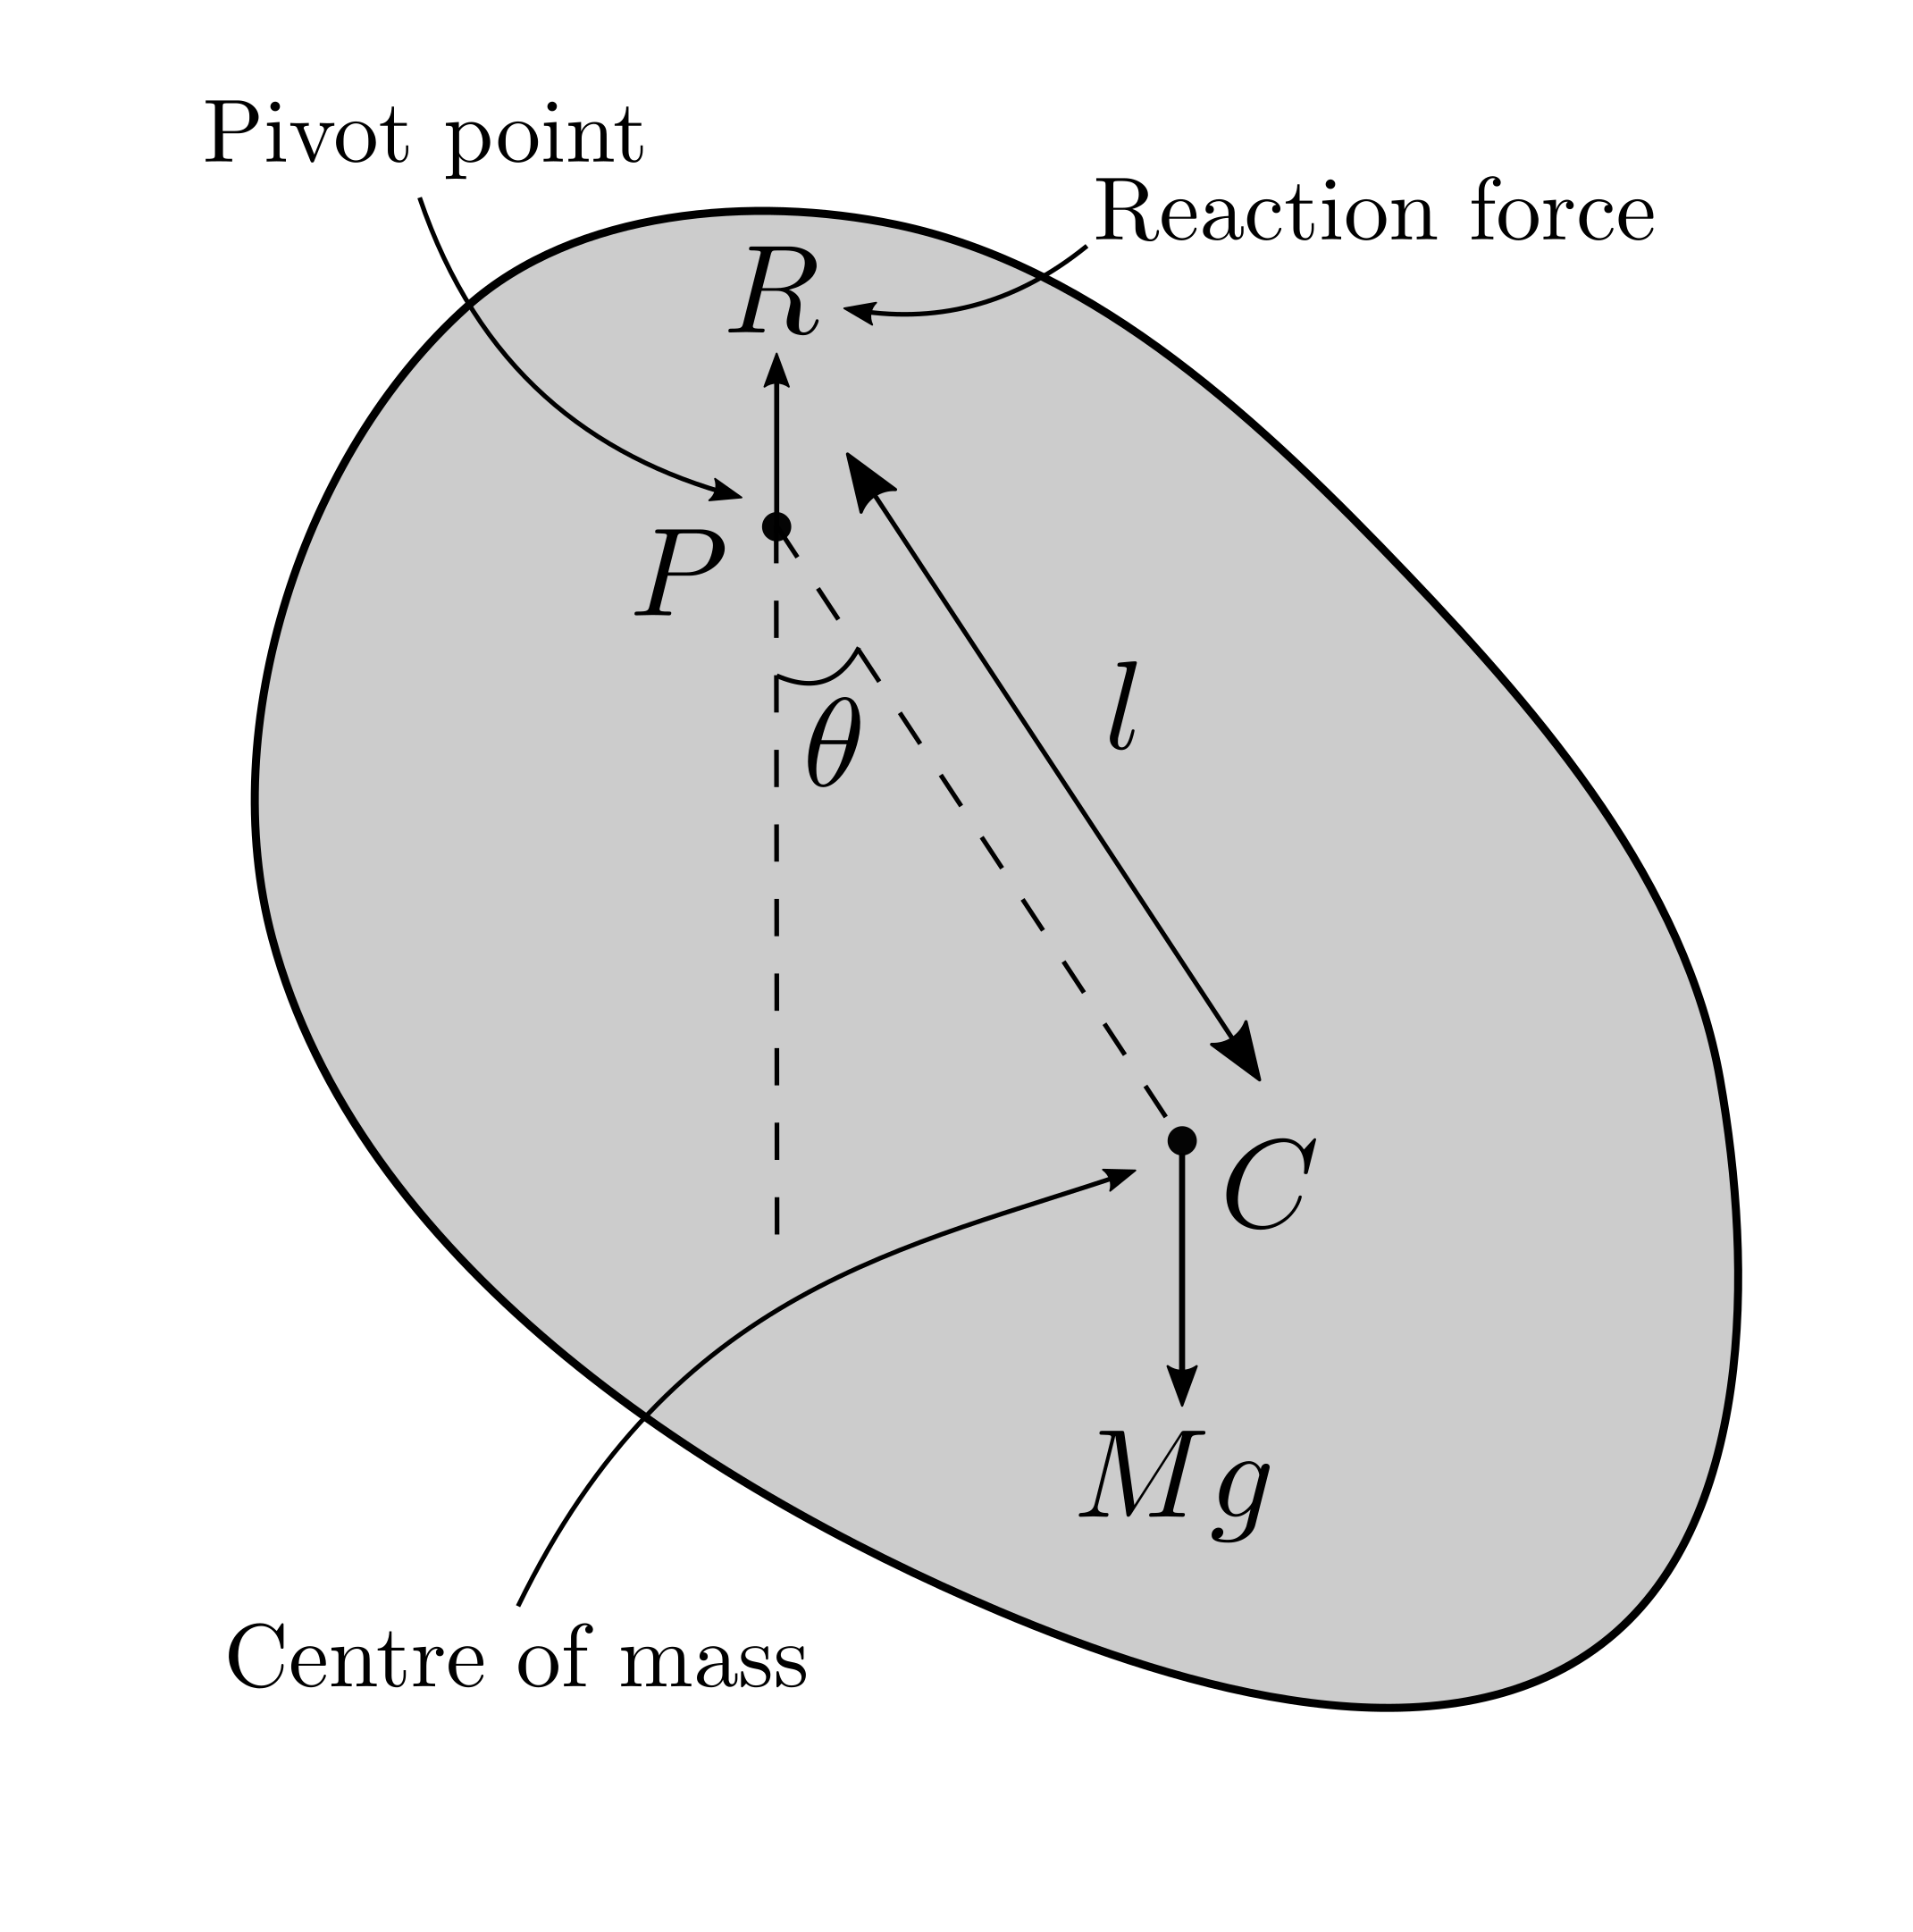
\includegraphics[scale=0.55]{figs/katers-pendulum/compoundPendulum.png}
        \caption{Schematic of a compound pendulum oscillating about a pivot $P$.}
\end{figure}

Kater's pendulum is a compound pendulum that is used to measure the local value of acceleration due to gravity. Before we describe how it does this, it is first important to understand what a compound pendulum is and how it behaves. In its most general sense, a compound pendulum is an extended object whose mass is distributed throughout its body. This is in contrast to a ``simple'' pendulum, where we assume all the mass is concentrated in the oscillating bob. The time period for small oscillations of such a pendulum is given by 
\begin{equation}
    T=2 \pi \sqrt{\frac{I_l}{mgl}},
    \label{eq:Tcomp}
\end{equation}
where $I_l$ is the moment of inertia of the body about the axis of rotation (at $l$), $g$ is acceleration due to gravity, $M$ is the total mass of the body, and $l$ is the distance between the pivot point and the centre of mass. (You should try deriving Equation~(\ref{eq:Tcomp}) using the torque balance equation.) Let $I_\text{CM}$ be the moment of inertia of a body about an axis passing through its centre of mass. By the parallel axis theorem, moment of inertia about any axis parallel to this is
\begin{equation}
    I_l=I_\text{CM}+ml^2,
    \label{parallel-axis-theorem}
\end{equation}
where $l$ is the distance from the centre of mass. $I_\text{CM}$ is usually simply written as $m k^2$, where $k$ is a quantity known as the radius of gyration, and which depends on the configuration of mass and the distance from the parallel axis through the centre of mass, about which the body is rotating. Thus, we have
\begin{equation}
    T = 2 \pi \sqrt{\frac{k^2 + l^2}{gl}}.
    \label{timeperiod-k}
\end{equation}

\begin{question}
\textbf{Question:} Write Equation~(\ref{timeperiod-k}) as a quadratic equation in $l$ (for a given period $T$). What do the roots of this equation correspond to?
\end{question}

From this, it should be clear that there are -- in principle -- an infinite number of points of suspension on a compound pendulum which have the same time period, all of which are at the same distance $l$ from the centre of mass. You can thus imagine drawing a circle of radius $l$ around the centre of mass, and every point on this circle would have the same time period $T_l$. What is less intuitive, however, is that there is a \textsl{second} circle, of radius $k^2/l$, such that all points suspended a distance of $k^2/l$ from the centre of mass \textsl{also} have the same time period $T_l$. There are thus two circles of ``conjugate'' points about which the time period is the same.

\begin{question}
\textbf{Question:} Using Equation~(\ref{timeperiod-k}), show that a point of suspension at a distance $d$ from the centre of mass, and a point of suspension at a distance $k^2/l$ from the centre of mass have the same time period of oscillation.

\textbf{Question:} Now, imagine a one-dimensional rod. Show that there are strictly four points of suspension which produce the same time period of oscillation:
\begin{equation}
    l, \quad -l, \quad \frac{k^2}{l}, \quad -\frac{k^2}{l}.
\end{equation}
Do all of them have to lie on the pendulum? Show that as one point of suspension approach the centre of mass, the other recedes from it.
\end{question}

We can use the Equation~(\ref{eq:Tcomp}) to measure the acceleration due to gravity by simply rearranging it so that 
\begin{equation}
    g=\frac{4\pi^2}{T^2}\frac{I_l}{ml}.
    \label{eq:T1}
\end{equation}

However, to get the value of $g$ from Equation~(\ref{eq:T1}), one has to know its moment of inertia accurately, which requires an accurate calculation of the body's mass distribution. Furthermore, using the formula as it stands requires us to know the position of the centre of mass precisely, since $l$ is measured with respect to this point. Doing this, however, is not easy. Kater's pendulum ingeniously sidesteps both of these problems through its design by depending primarily on the sum of two distances from the centre of mass in opposite directions, with the points between which distance is measured being the easily located knife-edges.

% \begin{question}
% \textbf{Question:} The knife-edges are assumed to have negligible masses. With respect to what do you think they are negligible?
% \end{question}

\section*{Theory}

Kater's Pendulum, shown in Figure~(\ref{fig:katers-setup}), consists of a thick rod (mass $M$) with two knife edges and two unequal masses, $M_1$ and $M_2$. These masses are adjustable; they can be moved along the rod.

 \begin{figure}[!htb]
        \centering
        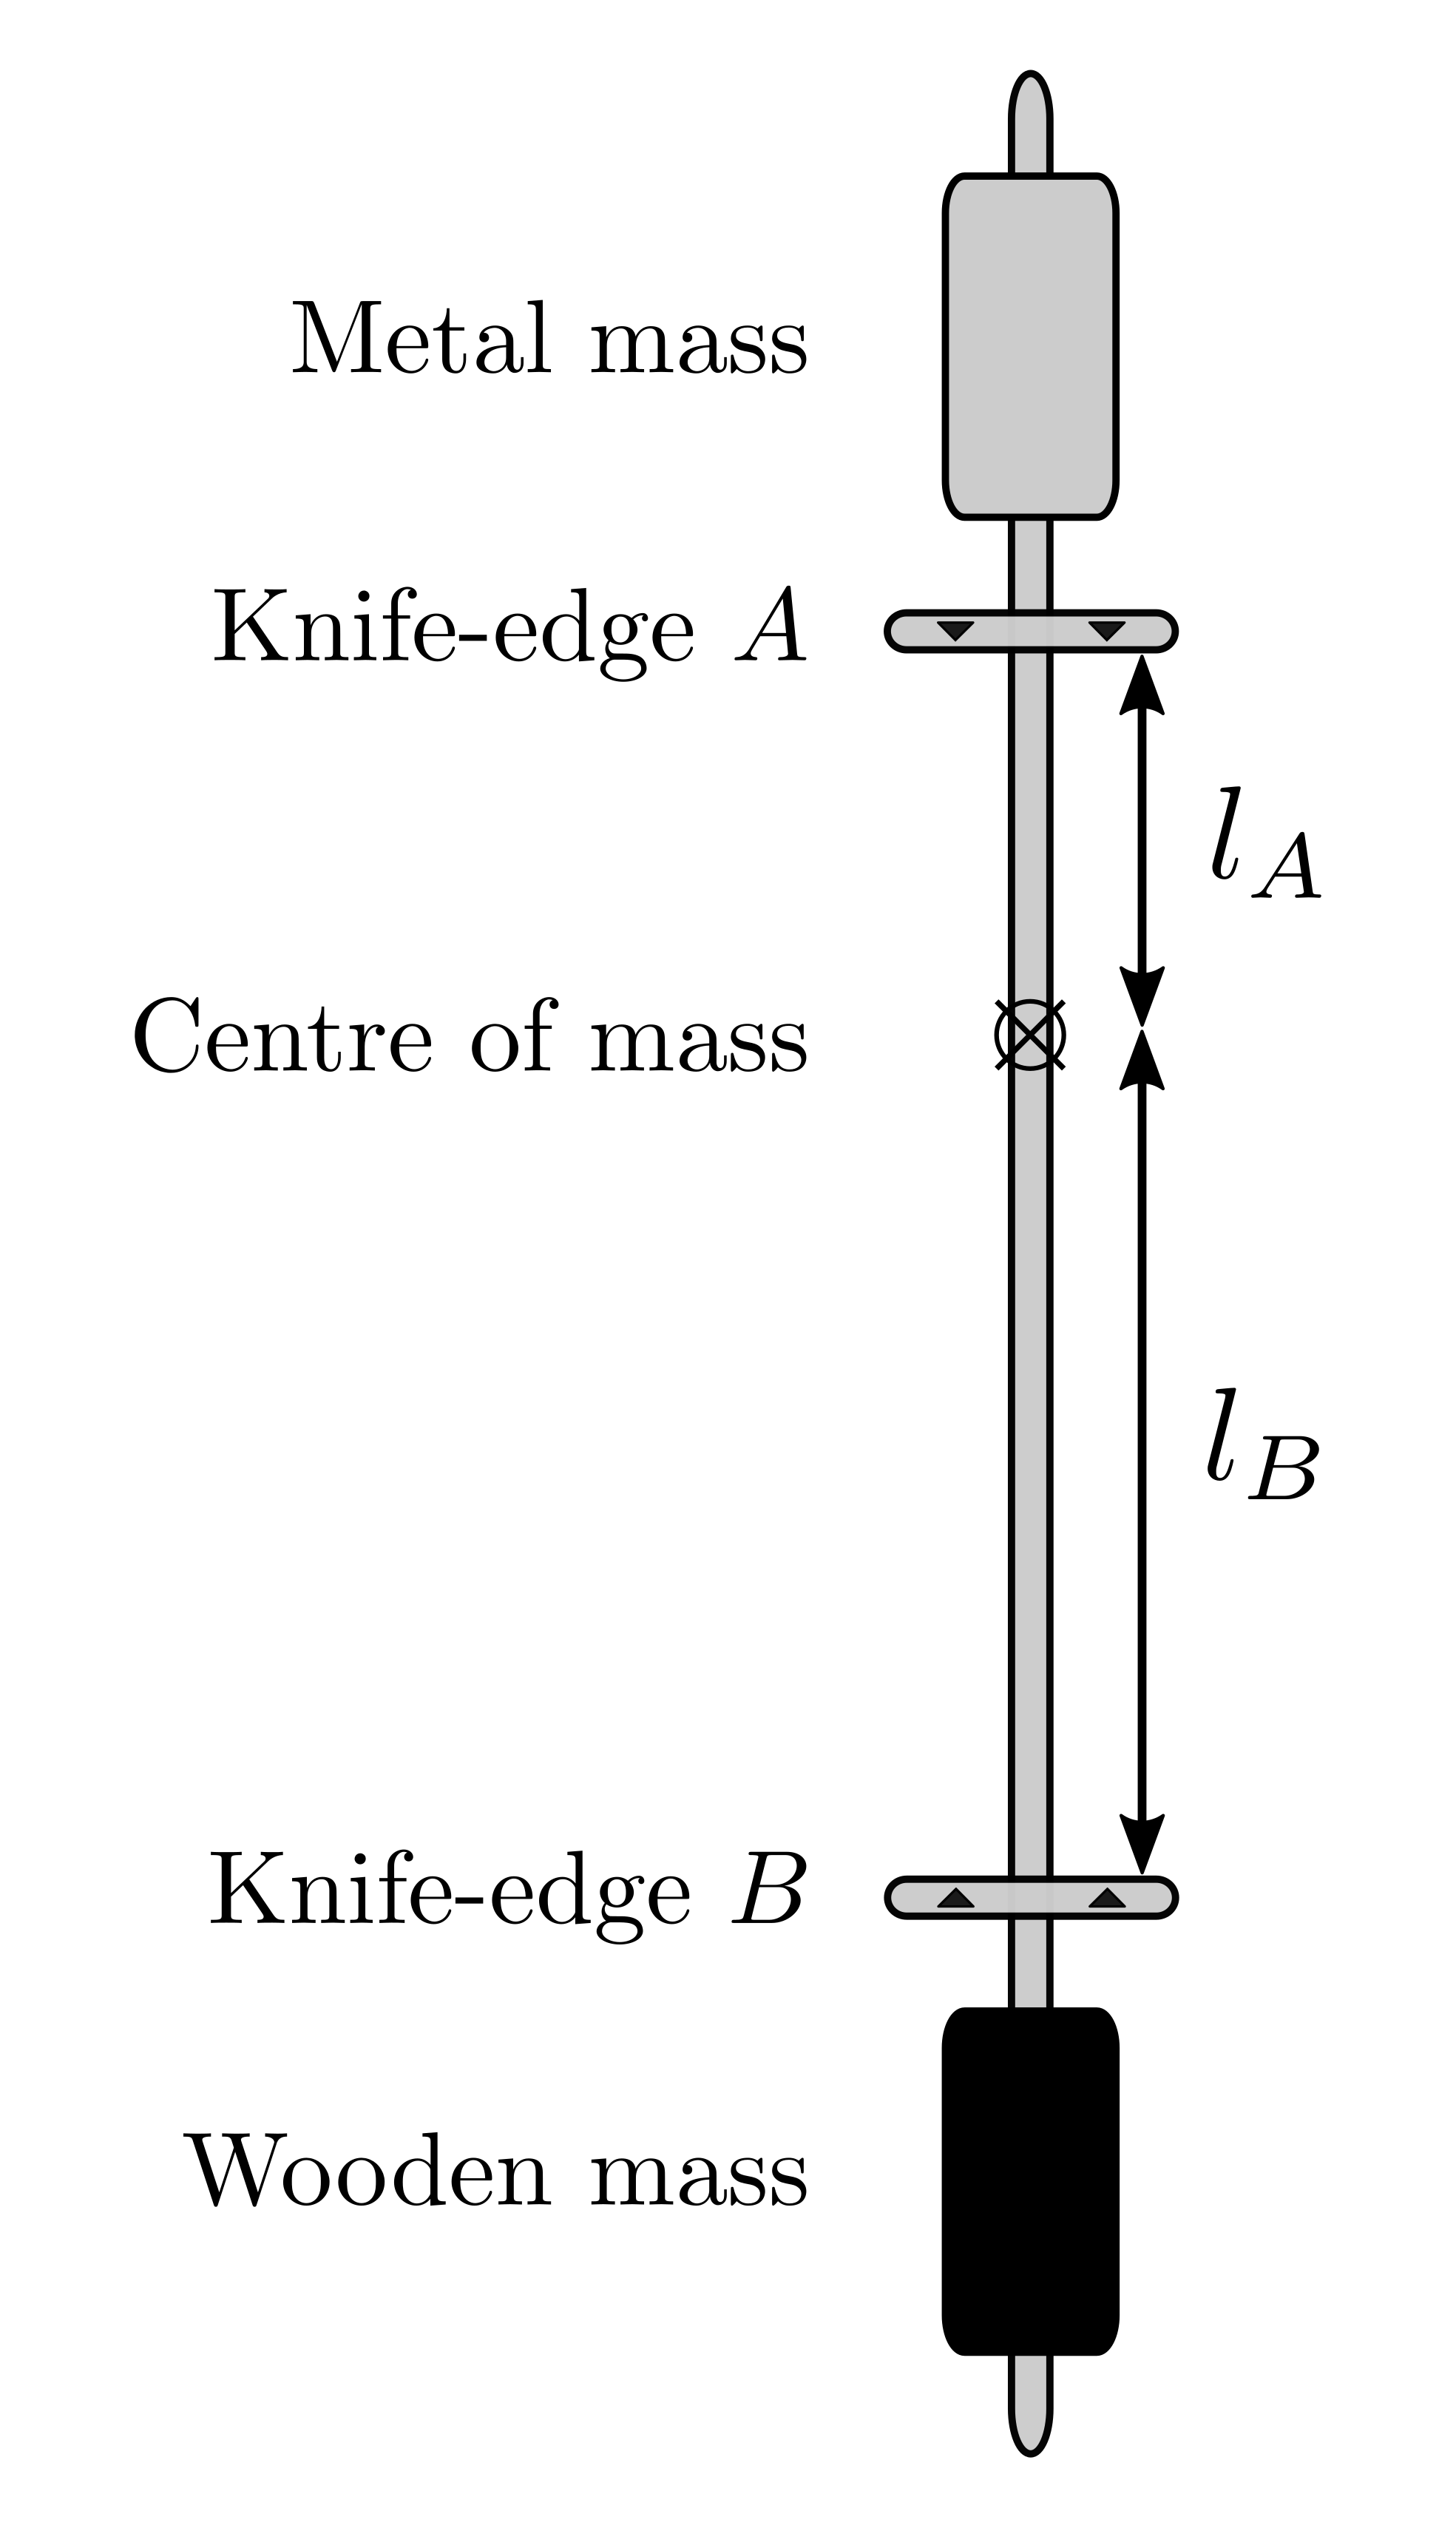
\includegraphics[scale=0.4]{figs/katers-pendulum/katers-setup.png}
        \caption{Schematic of the Kater's pendulum set-up. The pendulum is composed of a thick rod with two knife edges that allow it to be suspended from either end. Two unequal masses are placed on either side, and can be moved along the rod if necessary.}
        \label{fig:katers-setup}
\end{figure}

   
Consider the oscillations of such a pendulum in two different configurations:
\vspace{-\parskip}
\begin{enumerate}
    \item First, consider the pendulum suspended at the knife edge $A$, at a distance $l_A$ from the centre of mass, with some period of oscillation $T_A$.
    \item Next, consider the pendulum suspended about knife edge $B$, at a distance $l_B$ from the centre of mass, with some period of oscillation $T_B$.
\end{enumerate}

In each of the above cases, we can use the equation for the time-period of a compound pendulum and the parallel axis theorem -- Equations~(\ref{eq:Tcomp}) and~(\ref{parallel-axis-theorem}) respectively -- to relate the time period to the different parameters in the problem. In particular, if we denote the total mass of the pendulum $m$, we have
\begin{equation}
    \begin{aligned}
    T_A&=2\pi\sqrt{ \frac{I_{CM}+ m\,l_A^2} {m\,g\,l_A} },\\
    T_B&=2\pi\sqrt{ \frac{I_{CM}+ m\,l_B^2} {m\,g\,l_B} }.
    \end{aligned}
\end{equation}
We can eliminate $I_{CM}$ from the above equations, to get
\begin{equation}
    \frac{1}{g}=\frac{1}{4\pi^2} \left(\frac{T_A^2+T_B^2}{ 2(l_A+l_B)}+\frac{T_A^2-T_B^2}{ 2(l_A-l_B)} \right).
    \label{eqn:full-katers-g}
\end{equation}

Thus, we have managed to circumvent the issue of knowing the exact mass distribution of the pendulum, since we have a formula for $g$ that does not depend on the moment of inertia of our pendulum.

However, a further problem remains: in the second term above, we need to find $l_A - l_B$. This requires us to know the exact location of the centre of mass, which is difficult to measure precisely. We would thus like to eliminate this second term. We do this by realising that if we are able to choose our parameters such that $T_A = T_B$, the entire term will be set to zero. We know that that is a possibility because for any compound pendulum, there are two distances with the same oscillation period. The asymmetric mass distribution pushes the centre of mass away from the geometrical centre of the pendulum, and allows two conjugate points of suspension to be accessible.

% \begin{question}
% \textbf{Question:} Can you show why in this case $T_A = T_B$, but $l_A \neq l_B$?
% \end{question}

Thus, when we find the pivot points with same time periods, $T_A = T_B = T$, we can simplify the expression for $g$ to
\begin{equation}
    g = 4\pi^2 \left(\frac{l_A + l_B}{T^2}\right),
    \label{eqn:g-TA=TB}
\end{equation}

which provides us an accurate measurement of the acceleration due to gravity $g$ that does not require knowing either the mass distribution \textsl{or} the location of the centre of mass!

\begin{question}
\textbf{Question:} In the above formula, $l_A + l_B$ seems like the sum of two separate lengths measured with respect to the centre of mass. Experimentally, is this truly the sum of two lengths? 

\textbf{Question:} An important approximation of Equation~(\ref{eqn:full-katers-g}), probably derived by Bessel, is very useful to show that the expression for $g$ is much less sensitive to the location of the centre of mass, if $T_A = T_B$. Defining $T= (T_A + T_B)/2$, $\Delta T = (T_A - T_B)$, and $L=l_A + l_B$, show that if you ignore higher powers of $\Delta T$, $g$ can be very accurately approximated as
\begin{equation}
    g = \frac{8 \pi^2}{\dfrac{T_A^2 + T_B^2}{l_A + l_B} + \dfrac{T_A^2 - T_B^2}{l_A - l_B}} \approx \frac{4 \pi^2 L}{T^2} \left( 1 + \left( \frac{\Delta T}{T} \frac{L}{L-2l_A} \right)\right).
    \label{eqn:simplified-g}
\end{equation}
\end{question}

 
\section*{Experimental Setup}

\subsection*{Apparatus}

\begin{enumerate}
\itemsep0em
    \item A reversible Kater's Pendulum and a wall mount
    \item Assorted wooden and metal weights
    \item A stopwatch 
    \item A heavy wedge with which to determine the centre of mass of the pendulum rod
\end{enumerate}


\subsection*{Precautions}
\begin{itemize}
\itemsep0em
    \item The pendulum system is very heavy, make sure you do not drop it on your (or rather, anyone's) feet.
    
    \item The pendulum can be a spear. Make sure you carry it such that it does not hurt anyone.
    
    \item Make sure the knife edges are tightened (using a pair of pliers) to ensure that they do not slide during oscillations.
    
    \item The wooden weight has a tendency of slipping even when the screw is tightened by a pair of pliers. As a result, you might want to mark the position of the wooden block to keep track of it in case it moves. 
\end{itemize}


\section*{Procedure}

\subsection*{Part A}

You will begin this experiment by using the rod of the Kater's pendulum as a compound pendulum, and try to find four points on it which have the same time period $T$.

\begin{enumerate}
\itemsep0em
    \item Take the rod of the pendulum and a single knife-edge. Measure the centre of mass of the rod using a heavy wedge.
    
    \begin{question}
    \textbf{Question:} What is the radius of gyration $k$ of a rod of mass $M$? Assume the rod to be cylindrical; you will need to calculate its moment of inertia, and then use the definition of the radius of gyration.
    \end{question}
    
    \item Attach the knife-edge at one end of the rod, at some distance $l$ from the centre of the rod, and measure the time-period for 10 oscillations.
    
    \item Change $l$ by moving the knife-edge from one of the rod to the other, and measure the time period for 10 oscillations in each case.\
    
    \begin{imp}
    Ensure that the centre of mass is always below the knife-edge or the pendulum will topple over. You can do this by flipping the knife-edge as you cross the centre of mass.
    \end{imp}
    
    \item Plot a graph of $T$ vs. $l$, and show that there are four points which have the same time period. 
    
    \begin{question}
    \textbf{Question:} Why do we not need to take the moment of inertia of the knife-edge into account in this case?
    \end{question}
\end{enumerate}

\subsection*{Part B}

Next, you will use Kater's pendulum -- as it was intended -- to determine the local acceleration due to gravity $g$.

\begin{enumerate}
\itemsep0em
    \item Mark the centre of the rod and fix the masses at some fixed distance $d$ from this centre.
    
    \item Fix both the knife-edges some distance apart (call this $l$) on either side of the centre of the rod.
    
    \item By moving both masses with respect to their knife edges (i.e.\ the configuration of the system), change the centre of mass of the system. For each such position, measure $T_A$ and $T_B$ for 10 oscillations, and make a table of $T_A - T_B$, making sure you keep track of the sign. 
    
    \item You will notice that $T_A - T_B$ will change from positive to negative, thus indicating the configuration for which $T_A = T_B$. (Make sure you note down both $l_A + l_B$ and $l_A - l_B$.)

    \item Move to this configuration, and measure $T_A$ and $T_B$ again for 10 oscillations. If the difference is significant, make small adjustments until $T_A$ and $T_B$ are as close to each other as you can make them. One you have decided on your final configuration, measure $T_A$ and $T_B$ for 100 oscillations, making sure you count your oscillations carefully. 
    
    \begin{tip}
    If you make a mistake in counting the oscillations, this will show up in a comparison of the time periods obtained from 10 oscillations and those obtained from 100 oscillations.
    \end{tip}

\end{enumerate}

\subsection*{Part C}

Finally, you will perform a detailed analysis of the uncertainties on your result. 

\begin{imp}
There is a reason that the analysis of uncertainties in this experiment takes up an entire part of the experiment: it is extremely involved. Please make sure you pay attention to doing it well.
\end{imp}

For this analysis, it is essential to use the measured variables $T_A, T_B, L,$ and the larger length (say, $l_A$).

\begin{question}
\textbf{Question:} Why do you not need to use $l_B$ for the error analysis?

\textbf{Question:} Why is the \textsl{larger} length $l_A$ chosen?
\end{question}


\begin{enumerate}
    \item We begin with a result from uncertainty analysis: if a physical quantity $q$ is a function of multiple variables, i.e. $q = f(x,y,z)$, then the net uncertainty in $q$ -- which we denote $\Delta q$ -- can be computed using the formula
    \begin{equation}
        \Delta q^2 = \left(\pdv{f}{x}\right)^2 \Delta x^2 + \left(\pdv{f}{y}\right)^2 \Delta y^2 + \left(\pdv{f}{z}\right)^2 \Delta z^2.
    \end{equation}

    The above equation is just saying that the independent uncertainties due to the variables $x,y,$ and $z$ add in \textsl{quadrature}.
    
    \item Argue that the uncertainty in $g$ can thus be computed using the partial derivatives $$\pdv{g}{T_A},\quad \pdv{g}{T_B},\quad \pdv{g}{L},\quad \text{and} \quad \pdv{g}{l_A}.$$
    \begin{question}
        \textbf{Question:} In order to compute these derivatives, you should use Equation~(\ref{eqn:simplified-g}) and not the simpler Equation~(\ref{eqn:g-TA=TB}). Why?
        \textbf{Hint:} What assumption has been made when deriving Equation~(\ref{eqn:simplified-g})? 
    \end{question}

    \item Identify the uncertainties $\Delta T_A$, $\Delta T_B$, $\Delta L$, and $\Delta l_A$. Use these uncertainties to compute the error in $g$.
\end{enumerate}


\chapter{Air Track}

\section*{Objectives}

\begin{enumerate}
\itemsep0em
\item To study motion in one dimension in a near-frictionless set-up.
\item To attempt to verify Newton's three laws of motion.
\end{enumerate}


\section*{Introduction}

Newton's second law famously relates the externally applied force on an object to its acceleration,
\begin{equation}
    \vb{a} = \left(\frac{1}{m}\right) \vb{F}.
    \label{airtrack-newtonslaw}
\end{equation}

\begin{question}
 \textbf{Question:} You are probably a little uncomfortable about the way Equation~(\ref{airtrack-newtonslaw}) has been written. Can you explain why this way is, in some sense, superior to the common $\vb{F}=m\vb{a}$?
\end{question}

 From the above equations, it should be clear that if a body is given an initial velocity, and no external force is applied to it, it should continue to move at that velocity. In other words, its position should vary linearly with time.
 
 However, this clearly contradicts our everyday experience. Imagine placing your book on the table and giving it an initial velocity by pushing it and letting go: the book will, at best, move a little and come to rest. This does not, of course, contradict Newton's second law. The surface applies a force to the object that opposes its motion. Such ``frictional'' forces are notoriously difficult to take into account, and so if we want to study simple one dimensional systems, it would be helpful to minimise them as far as possible. However, if you imagine an object in outer space, it is not difficult to see that giving it a push will cause it to move at a constant velocity.
 
 It is not possible for us to conduct this experiment in outer space. However, what essentially distinguishes the environment in outer space from the table-top is the presence of friction. A device that almost eliminates friction if the air track, which simulates a low-friction environment by creating a ``cushion'' of air on which an object (called a ``rider'') may float. 
 
\begin{figure}[!htb]
     \centering
     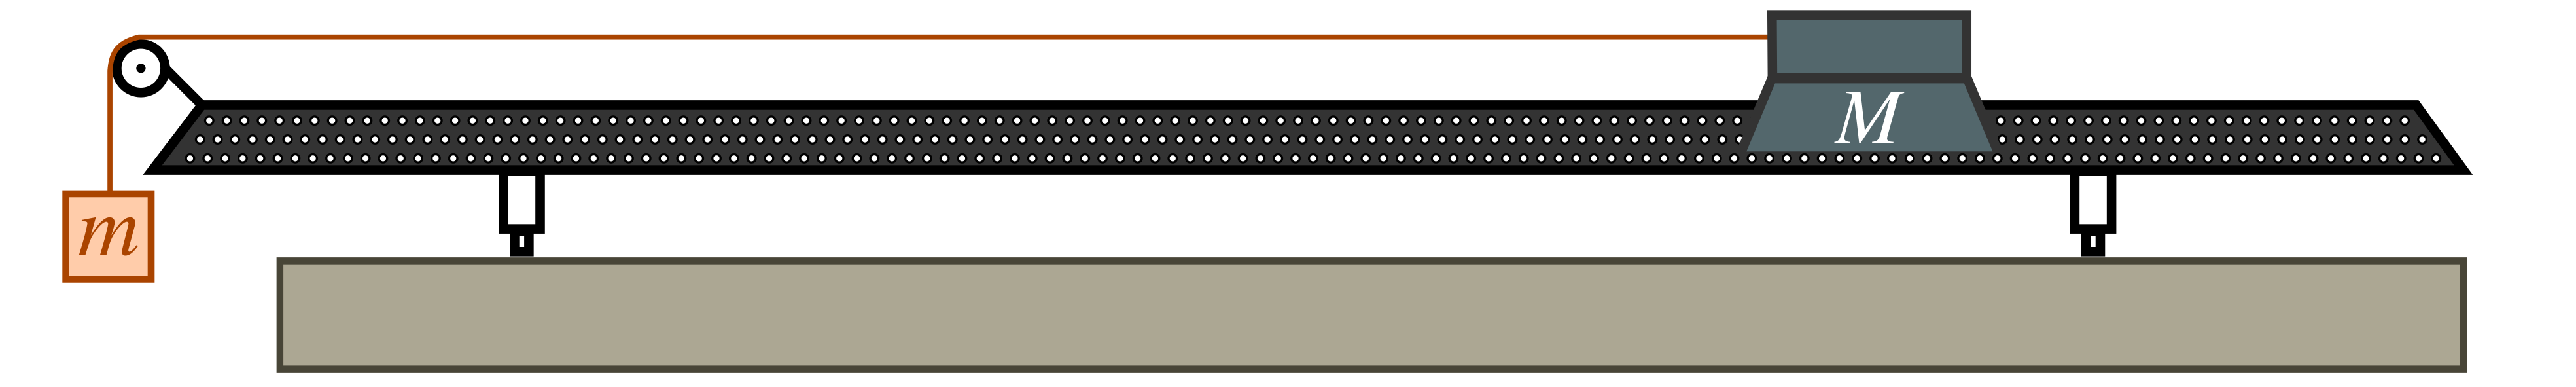
\includegraphics[width=0.9\textwidth]{figs/airtrack/airtrack-setup.png}
     \caption{Schematic of the set-up. A rider of mass $M$ floats on the track, and is connected to a mass $m$ through a pulley and an inextensible string. As the mass $m$ is allowed to fall, the rider experiences a constant acceleration. }
     \label{fig:airtrack}
 \end{figure}

\section*{Theory}

\subsection*{Uniformly accelerated motion}

\begin{question}
    \textbf{Question:} Consider an object of mass $m$ acted on by a constant force $F_0$. Show, by integrating Newton's second law, that the object's velocity and position vary as
    \begin{equation}
    \begin{aligned}
     v(t) &= v(0) + \left(\frac{F_0}{m}\right) t,\\
     x(t) &= x(0) + v(0) t + \frac{1}{2} \left(\frac{F_0}{m}\right) t^2.
    \end{aligned}
    \end{equation}
\end{question}

To test the above equations, we impose a constant force on the rider. Consider setting the air track up as shown in Figure~(\ref{fig:airtrack}). Connect a mass $m$ to the rider (of mass $M$) with an inextensible string. When the mass $m$ is released, the only horizontal force on the rider comes from the tension $T$ on the string, and so 
\begin{equation}
M a = T.
\end{equation}

\begin{question}
\textbf{Question:} Can you argue that the two blocks must accelerate at the same rate $a$? What assumptions do you need to make for this?
\end{question}

The hanging mass $m$ feels both gravity (downwards) and tension $T$ (upwards), so that
\begin{equation}
m a = mg - T.
\end{equation}

\begin{question}
\textbf{Question:} Show that by measuring the acceleration of the rider, one can measure the acceleration due to gravity $g$, since
\begin{equation}
g = a \left(\frac{M+m}{m}\right).
\end{equation}
\end{question}

\subsection*{Conservation of momentum}

When such a low-friction environment ensures that (almost) no external forces are acting on the object, Newton's second law tells us that the quantity $m\times v$ is a constant. When we have a single object, this just tells us that -- when there are no external forces acting on the object -- its momentum stays constant. If, in addition, the mass of the object is constant, this is just a statement that the velocity remains constant.

Such ``momentum conservation'' applies to a single object, but it is a lot more interesting to look at a situation with at least two interacting objects. Consider two objects moving at constant velocities (say $v_1$ and $v_2$) which collide. From Newton's third law, the force of the first on the second (say, $F_{12}$) is equal and opposite to the force of the second on the first ($F_{21}$). Thus,
\begin{equation}
F_{12} = - F_{21}.
\end{equation}

If we consider that the forces act over a small time interval $\Delta t$, it follows that the impulses experienced by the two objects are also equal in magnitude and opposite in direction, i.e.\ 
\begin{equation}
\begin{aligned}
 F_{12} \Delta t &= - F_{21} \Delta t,\\
 m_1 \Delta v_1 &= - m_2 \Delta v_2,
 \end{aligned}
\end{equation}
where in the last case we have simply used the definition of the acceleration. Thus, we can see that the change in momentum of each mass is equal in magnitude, but opposite in sign: momentum is \textsl{transferred} from one object to the other.

\begin{question}
\textbf{Question:} In the above case, show that the velocities before and after the collision are related by:
\begin{equation}
m_1 v_1^\text{before} + m_2 v_2^\text{before} = m_1 v_1^\text{after} + m_2 v_2^\text{after}
\end{equation}
\end{question}

\subsection*{Elastic and inelastic collisions}

It may have struck you that in the earlier case we seemed to imply that after the collision the objects moved away at different velocities, and thus remained \textsl{distinct} (consider two billiard balls colliding). However, from real world experience you have often seen another case: collisions where the two objects ``stick'' together, and thus move at together at the same velocity after the collision (consider two lumps of clay thrown at each other). Consider both these cases: since we could engineer it such that the objects (billiard balls or lumps of clay) have the same masses and the same velocities, and since we know that the results after the collisions are clearly different, there must be some way to distinguish between them.

You will show, in your course on \textsl{Classical Mechanics}, that the distinction between such collisions is to do with another conserved quantity: energy. In particular, the kinetic energy (or the energy that an object possesses by virtue of its motion) is given by \begin{equation}
\text{KE} = \frac{1}{2} m v^2.
\end{equation}

We can use the kinetic energy to classify collisions into two types:
\begin{enumerate}
 \item \textbf{Perfectly elastic} collisions in which both momentum and kinetic energy are conserved. In other words, if two masses $m_1$ and $m_2$ and velocities $v_1$ and $v_2$ collide elastically and move away with velocities $v'_1$ and $v'_2$, then
 \begin{equation}
 \begin{aligned}
     m_1 v_1 + m_2 v_2 &= m_1 v'_1 + m_2 v'_2,\\
    \frac{1}{2}m_1 v_1^2 + \frac{1}{2} m_2 v_2^2 &= \frac{1}{2}m_1 {v'_1}^2 + \frac{1}{2} m_2 {v'_2}^2.
 \end{aligned}
 \end{equation}
 \item  \textbf{Perfectly inelastic} collisions in which momentum is conserved, but kinetic energy is not conserved. In other words, if the masses stick together to form a mass of $m_1 + m_2$ moving at some velocity $V$, then
 \begin{equation}
 \begin{aligned}
     m_1 v_1 + m_2 v_2 &= (m_1 + m_2)V,\\
    \frac{1}{2}m_1 v_1^2 + \frac{1}{2} m_2 v_2^2 &\neq \frac{1}{2}(m_1+m_2) V^2.
 \end{aligned}
 \end{equation}
\end{enumerate}

\begin{imp}
It is important to realise that while \textsl{kinetic} energy is not conserved, this does not mean \textsl{energy} is not conserved. Since energy can take different forms, some of the initial kinetic energy may go into deforming the objects, or producing heat. In general, most collisions are inelastic (though not \textsl{perfectly} inelastic), and some energy is always lost to the environment.
\end{imp}

\begin{question}
 \textbf{Question:} Perfectly elastic collisions generally only occur at the atomic scales. The example of two billiard balls is not a perfectly elastic collision. Where do you think the lost kinetic energy goes?
 
 \textbf{Question:} Show that in perfectly inelastic collisions above, the ``loss'' in kinetic energy is can be written as 
 \begin{equation}
     \text{Loss in KE} = \frac{1}{2} \mu \, (v_2 - v_1)^2.
 \end{equation}
 Where you need to determine $\mu$ (called the \textsl{reduced mass} of the body). What do you think this means? 
\textbf{Hint:} Imagine placing yourself in the reference frame of the centre of mass of the two objects.
\end{question}




\section*{Experimental Setup}

\subsection*{Apparatus}

\begin{enumerate}
\itemsep0em
\item A 2 metre-long air track
\item A blower to pump air through the track
\item Assorted accessories including riders and their attachments (shown in Figure~(\ref{fig:airtrack-accessories}))
\item Two photogates and associated their cables (\textsl{Vernier} or \textsl{Indosaw})
\item Retort stands to position the photogates
\end{enumerate}


\subsection*{Description}

\begin{figure}[!htb]
    \centering
    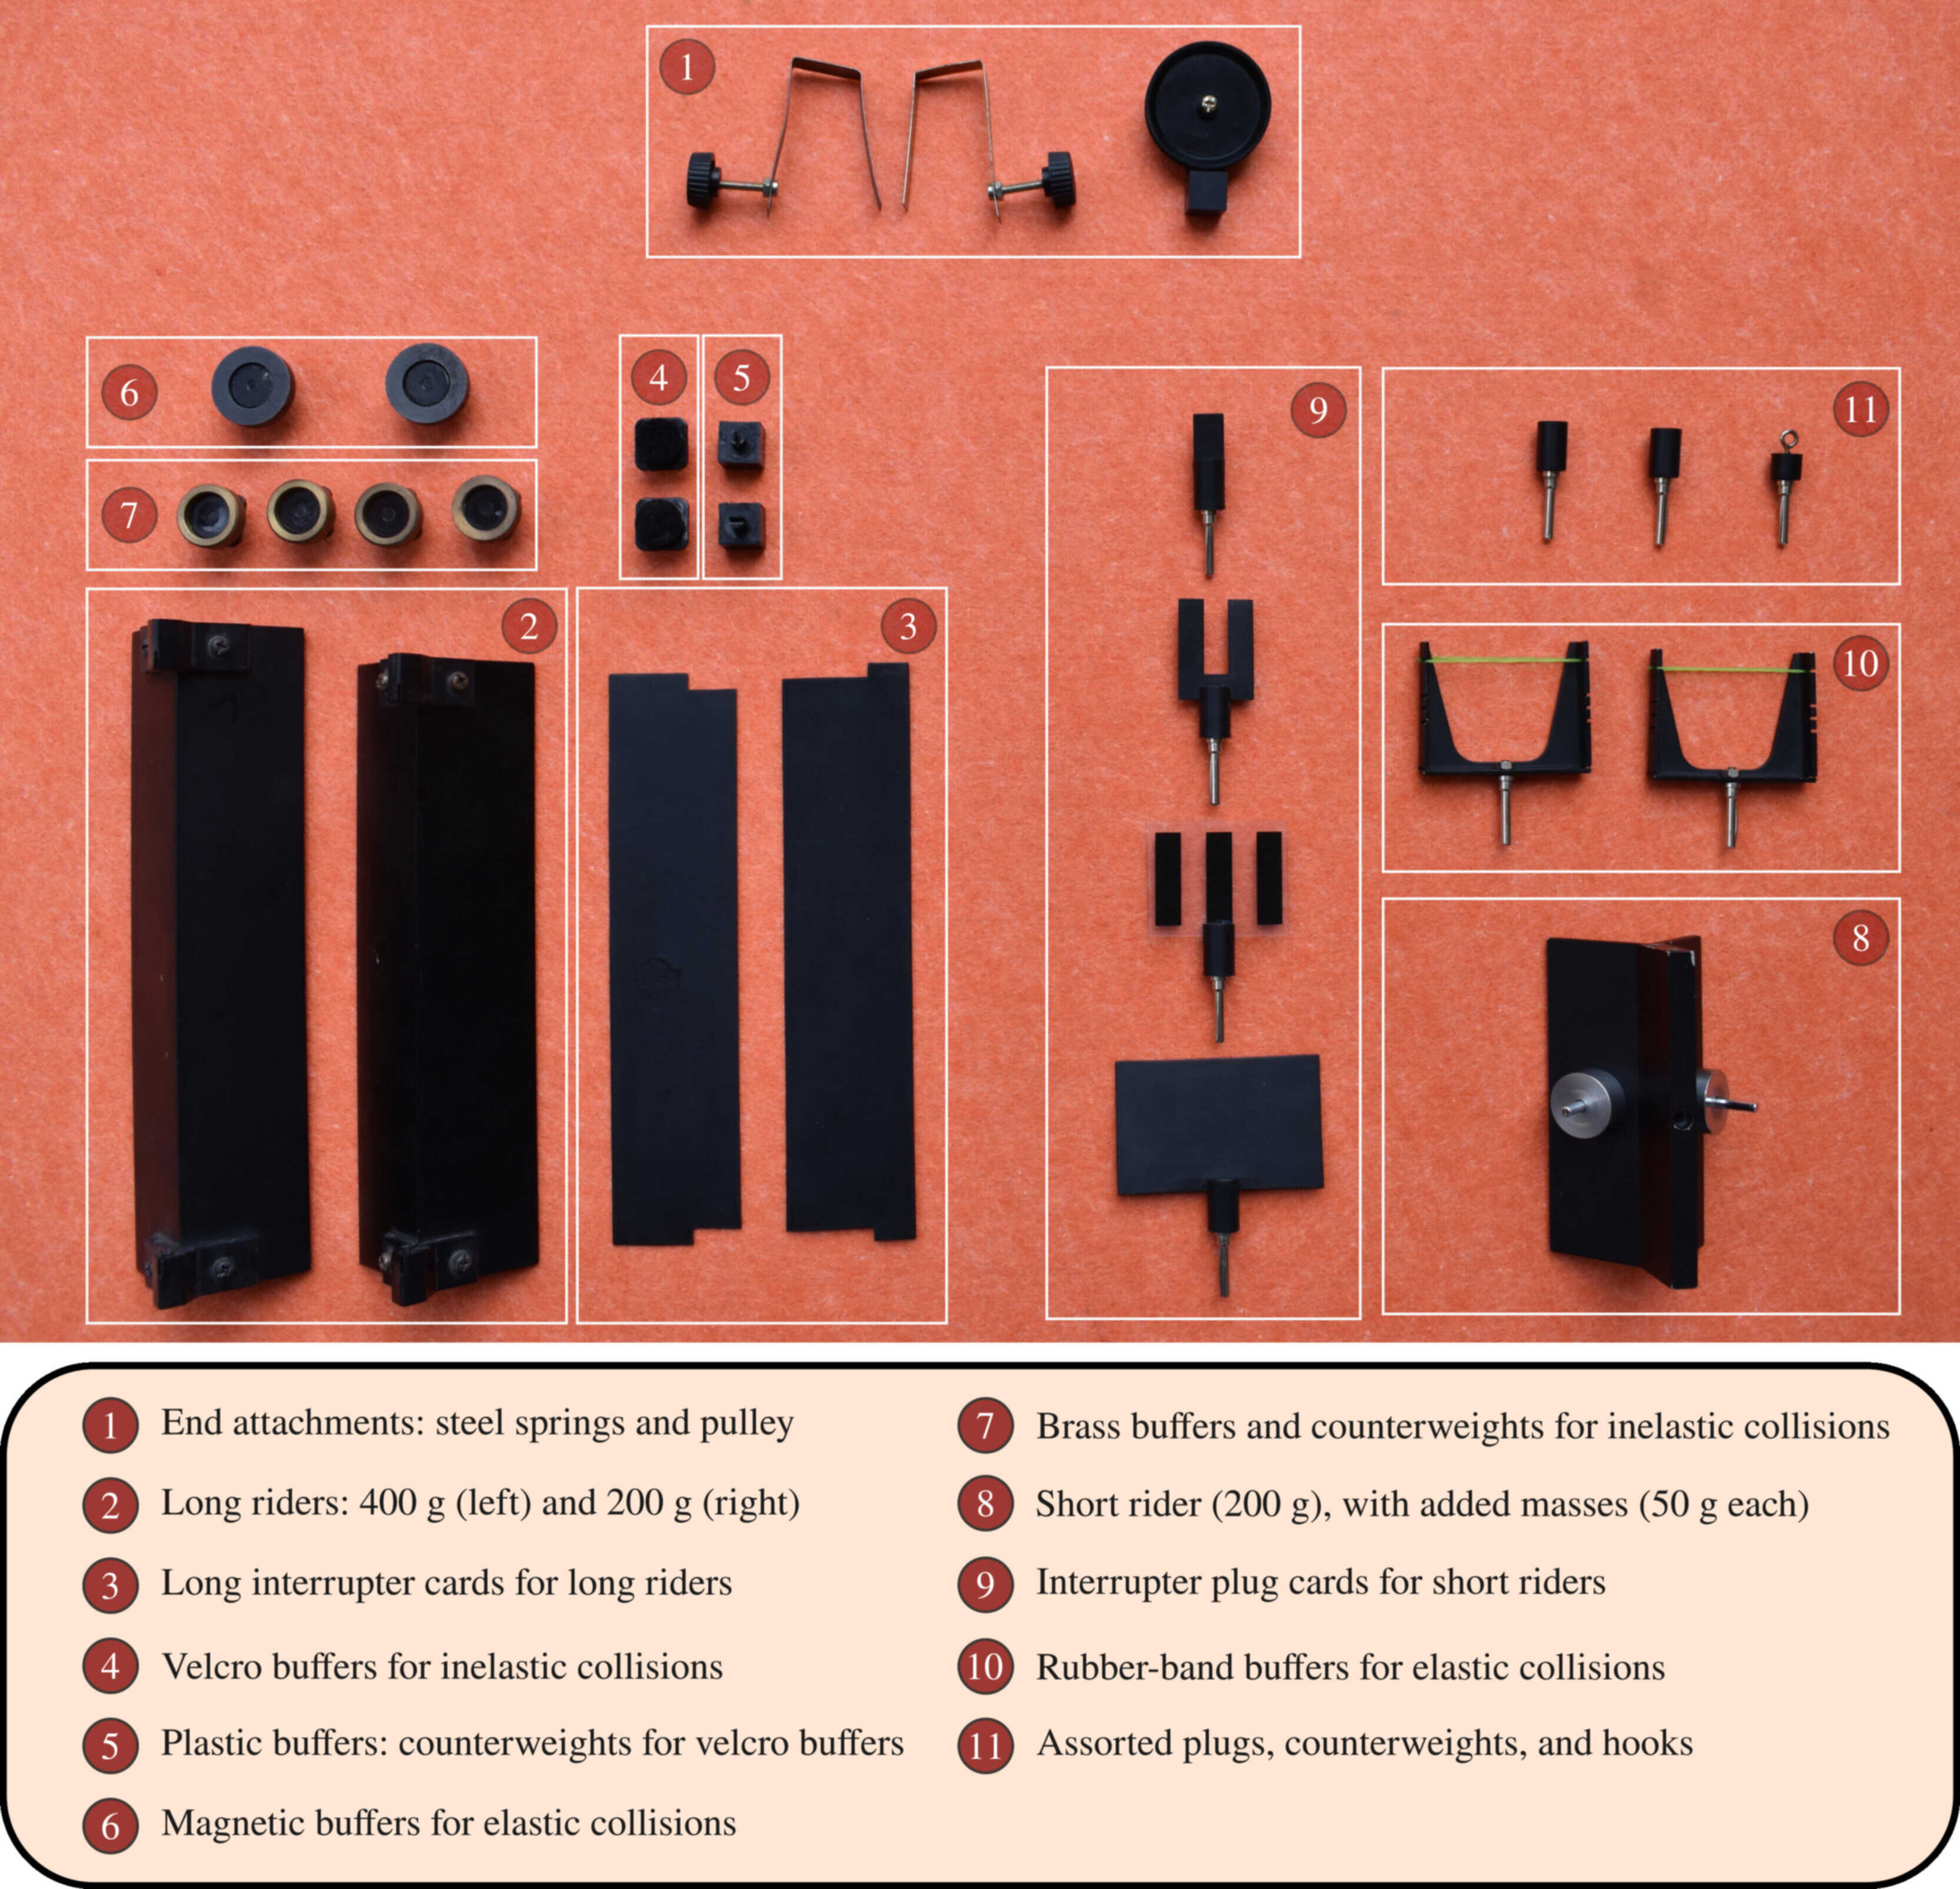
\includegraphics[width=\textwidth]{figs/airtrack/airtrack-accessories.jpg}
    \caption{Accessories for the air track. The end attachments are placed at either end of the track. The remaining accessories are placed on one of the two different types of riders, long or short. The long riders come in two types: the heavier 400 g rider is slightly longer than the 200 g rider. On the left are all the attachments for the long riders, and on the right are all the attachments for the short riders.}
    \label{fig:airtrack-accessories}
\end{figure}

\subsubsection*{The air track}

The air track, as explained, can be used as a low-friction environment for kinematics experiments. Compressed air is injected into the cavity beneath the track. Since this cavity is sealed, the air can only escape through the small holes on the track. This provides a force strong enough to lift the riders, drastically lowering the contact friction.

Connect the hose from the blower to the air track and turn it on. The speed of the blower (and thus the pressure on the rider) can be controlled by the knob on the blower.

The first step is to level the track, which you will do with a spirit level by adjusting its legs. A good way to test if the track is levelled and the pressure is sufficient is simply to place one of the riders on it and observe its behaviour. If the rider floats gently above the track and shows no preference for the right or left end, your air track is ready to use. 

\begin{tip}
Do not be tempted to keep the blower at maximum: too much pressure will cause more air to escape near the inlet than elsewhere, which will cause turbulence and destabilise experiments. On the other hand, using the bare minimum pressure requires you to be sure that the track is completely free of scratches or dirt on its surface. Try to find a middle ground before you start.
\end{tip}

\subsubsection*{End attachments}

The steel springs and pulley given with the set-up may be attached to the ends of the air track. The springs can be used to launch the riders, or to allow them to bounce back nearly elastically. The pulley may be placed on one end to change the direction of an applied force from vertical to horizontal.

\subsubsection*{Riders}

\begin{figure}[!htb]
    \centering
    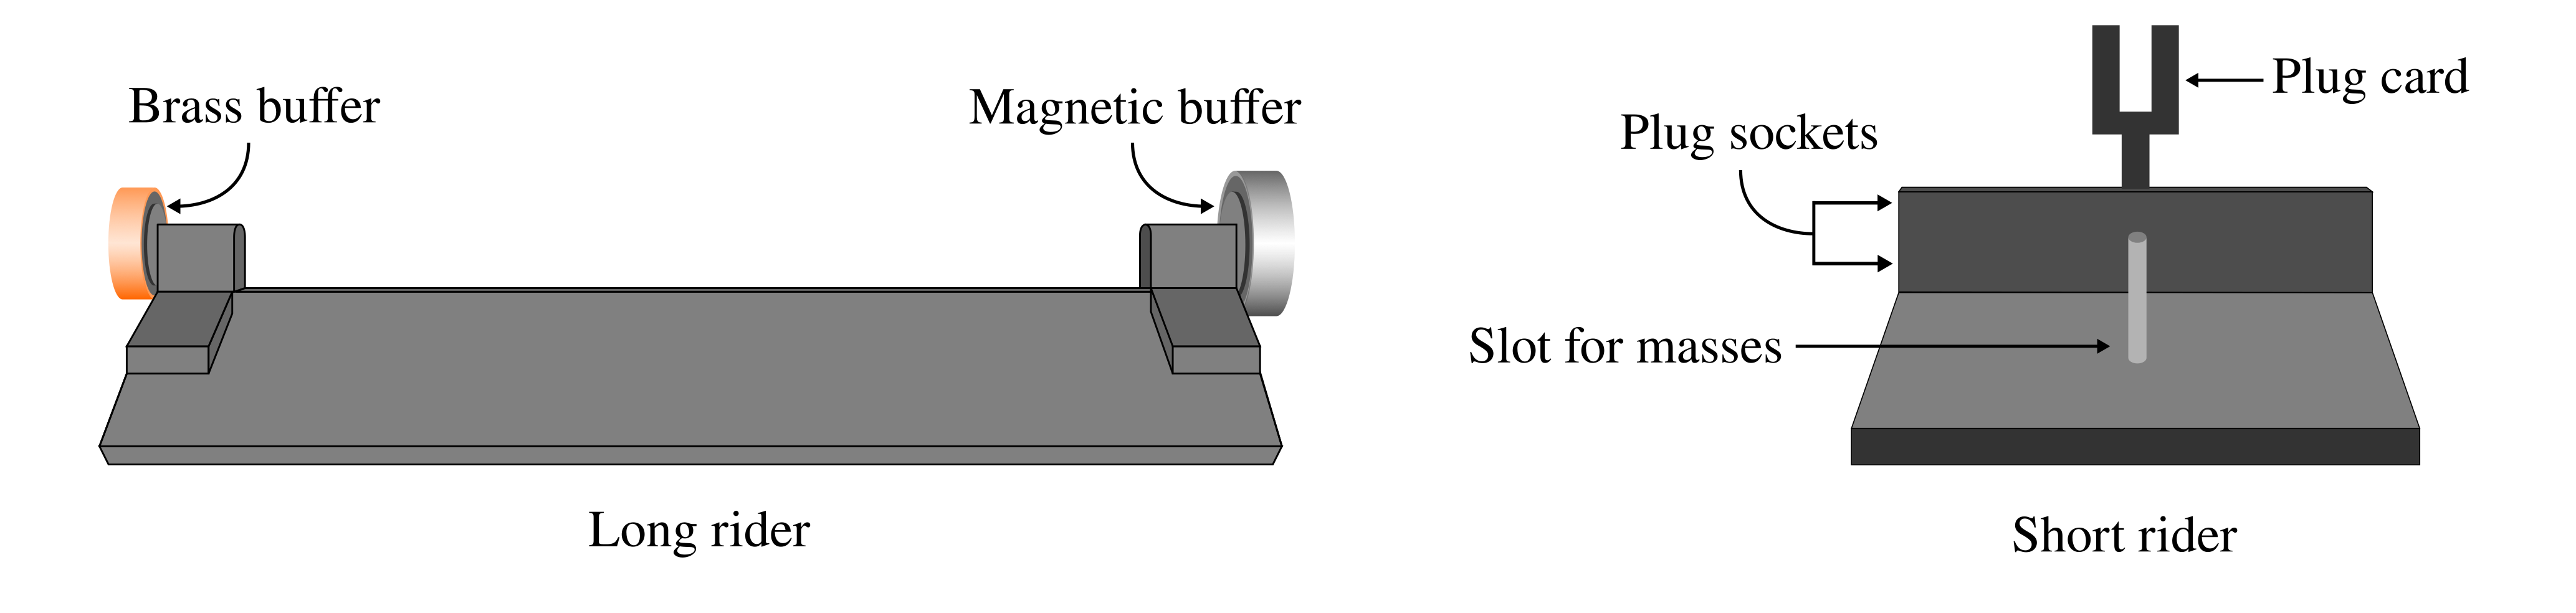
\includegraphics[width=\textwidth]{figs/airtrack/airtack-riders.png}
    \caption{Two sizes of riders, long and short. Short riders weigh roughly 200 g, and have slots on either side on which masses may be placed to increase the rider's weight. Two types of long riders are provided, one weighing 200 g and the other 400 g. }
    \label{fig:airtrack-riders}
\end{figure}

The air track has three different types of riders, on top of which the different interrupter cards and prongs may be added when working with the photogates. The riders can be distinguished by their mass and size:

\begin{enumerate}
    \item \textbf{Short rider} ($\sim 200$ g) with attachments on either side to add masses. (Make sure that the masses are added symmetrically on both sides.) The hole on the top may be used to attach the photogate flags to the rider.
    
    \item \textbf{Long rider} ($\sim 200$ g) along the top of which the short interrupter cards may be slotted.
    
    \item \textbf{Long rider} ($\sim 400$ g) along the top of which the longer interrupter cards may be slotted.
\end{enumerate}

\subsubsection*{Buffers and counterweights}

The riders have two holes on their edges, at different heights, to which different buffers may be attached. 

\begin{imp}
Whenever a buffer is added on one side, a counter-weight or plug must be added on the other side, to avoid the air track leaning to one end. If this happens, there will be an unbalanced horizontal force which will make the rider move in the direction it leans.
\end{imp}

\begin{enumerate}
    \item \textbf{Rubber-band bumpers} may be connected to the riders to simulate nearly elastic collisions. In order to do this, the bumpers will each need to be aligned at 45$^\circ$ to the riders in opposite directions, such that the elastic bands are perpendicular to each other, ensuring that they have plenty of room to stretch.
    
    \item \textbf{Magnetic buffers} may also be connected for nearly elastic collisions. As they act over a distance, no physical contact is made, and thus no energy can be lost to heat or sound.
    
    \item \textbf{Brass buffers} may be used as counterweights when the magnetic buffers are used for elastic collisions, but can also be used for inelastic collisions, as they lose energy as heat and sound when they collide. In this case, take care to add the magnets on the other side, as counterweights.
    
    \item \textbf{Velcro buffers} may be used to simulate perfectly inelastic collisions, as they will force the vehicles to stick together after impact. When these are used, appropriately sized plastic buffers should be used as counterweights.
    
    \item \textbf{Plastic buffers} are generally used as counterweights, but are suitable for inelastic collisions as well, provided the Velcro buffers are used as counterweights.
\end{enumerate}


\subsubsection*{The photogates}

\begin{figure}[!htb]
    \centering
    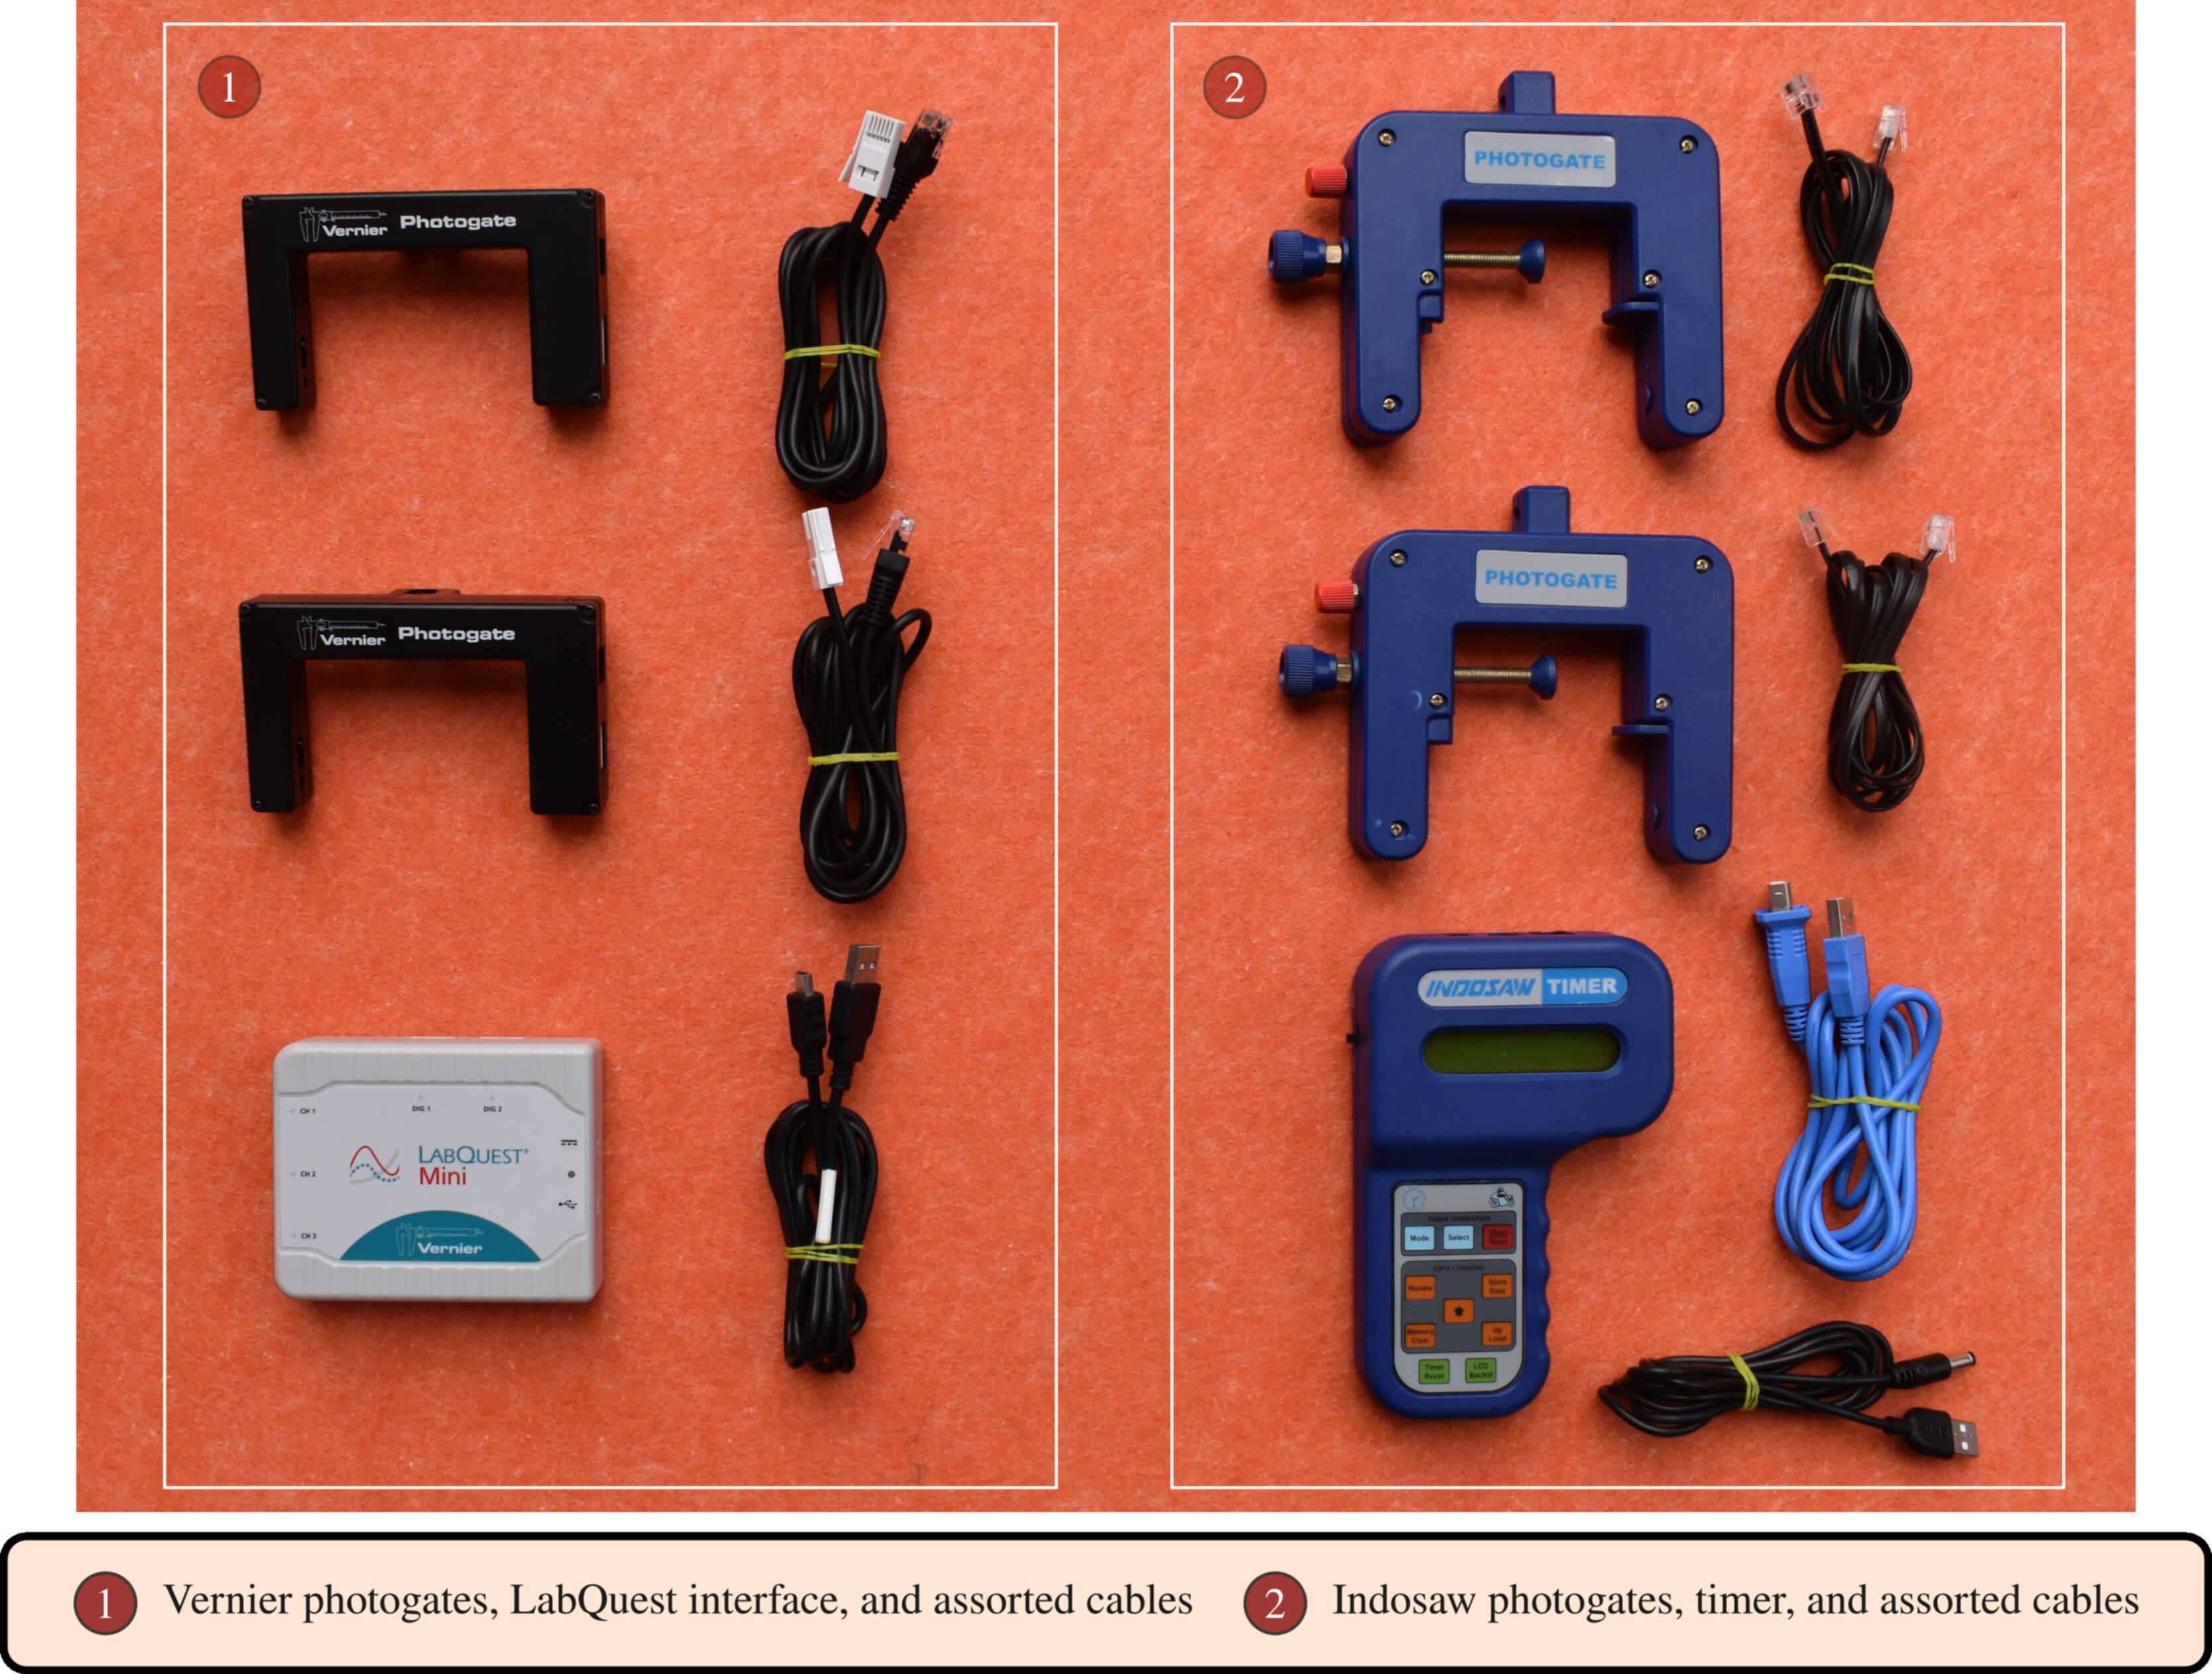
\includegraphics[width=\textwidth]{figs/airtrack/airtrack-photogates.jpg}
    \caption{Available photogates. The Vernier photogates (left) are controlled through the LabQuest interface which connects to a computer, while the Indosaw setup (right) has its own timer.}
    \label{fig:airtrack-photogates}
\end{figure}

Photogates allow for extremely accurate timing of events within physics experiments. They work by changing the state of their output signal whenever an object comes in between their infrared sensors, which allows us to measure the time interval $\Delta t$ the object takes to pass through the gate. If the object is sufficiently small -- and has a known length $\Delta x$ -- then we can find a good approximation of its instantaneous velocity,
\begin{equation}
    v \approx \frac{\Delta x}{\Delta t}.
\end{equation}
If the instantaneous acceleration is required, an interrupter with two prongs may be used. By measuring the change in velocity between these prongs $\Delta v$ and the change in time $\Delta t$, the instantaneous acceleration may be approximated as
\begin{equation}
    a \approx \frac{\Delta v}{\Delta t}.
\end{equation}

You have two types of photogates, \textsl{Vernier} and \textsl{Indosaw}, shown in Figure~(\ref{fig:airtrack-photogates}). The Vernier photogates will be used with the \textsl{LabQuest} interface and its data can be collected and analysed using the \textsl{LoggerPro 3} software. Each gate has an input port so multiple gates can be connected in a ``daisy-chain'' configuration. With the \textsl{LabQuest} interface and Vernier gates, up to four gates can connect to a single interface channel. The Vernier photogate also has a laser gate mode, which requires the addition of a common pen laser, which is directed into the laser port. The laser may be some distance from the gate, so that you can measure the speed of larger objects.


\begin{tip}
    Tutorials for the Vernier photogates can be found online,\footnote{\nolinkurl{https://www.vernier.com/training/videos/play/?video=201}} as can the manual. Make sure you go through them before collecting data to avoid making common mistakes.
\end{tip}

\subsection*{Precautions}
\begin{itemize}
\itemsep0em
\item \textbf{The air track must be level}! First use a spirit level to level the track roughly, then place a rider at different points on the track and adjust the legs until it shows no preference for the left or right end of the track.

\item Make sure the track's surface is clean, and none of the holes are plugged by dirt.

\item Ensure that the rider never tilts towards one direction. If this happens, you have either placed the weights asymmetrically or forgotten the counterweights.

\item If the rider wobbles, the air pressure is too high.

\item The collisions need to be as gentle as possible. A large source of uncertainty is the transfer of energy to the air track and table.
\end{itemize}

\begin{imp}
\textbf{Inherent errors:}
The riders are supported by a thin film of air approximately 0.01 cm thick. This film exerts a viscous drag on moving surfaces which should -- in theory -- cause the rider to gradually slow down until it comes to rest. However, practically, the rider oscillates around a position midway between the air holes. An air track with a practically infinite number of air holes would eliminate this problem, but this is not reasonable. Increasing the thickness of the film of air would reduce the coefficient of friction, but this would be at the expense of the rider's stability. Another potential source of error is the straightness of the air track. While an ideal air track should not sag, our tube is still heavy enough to sag slightly under the force of gravity. 
\end{imp}


\section*{Procedure}
\subsection*{Part A}

In the first part of this experiment, you will attempt to verify Newton's first law, showing that when an object experiences no external force, it travels in uniform rectilinear motion.

\begin{enumerate}
    \item Set up the metal springs at either end of the air track. Placing the rider at one end of the track, gently push it against the spring and let go.
    
    \item Measure the velocity of the rider using the photogates at two different points in its trajectory, and measure its velocity at both points.
    
    \item Repeat this for different initial velocities.
\end{enumerate}

\begin{question}
 \textbf{Question:} Assuming the steel spring to be ideal, show that the velocity of the rider is directly proportional to its initial displacement of the spring.
\end{question}

\subsection*{Part B}

Next, you will attempt to verify Newton's second law showing that under a constant force, the riders move with a constant acceleration.

\begin{enumerate}
    \item Remove one of the steel springs and connect the pulley. Pass a long string across the pulley and connect it to the rider at one end, and a slotted mass at the other, as shown in Figure~(\ref{fig:airtrack}).
    
    \item With the rider at one end, drop different masses and measure the change in velocity between two points along the riders trajectory to measure the acceleration.
    
    \item Plot a graph to calculate the acceleration due to gravity.
\end{enumerate}

\subsection*{Part C}

Finally, you will attempt to verify Newton's third law by colliding different riders together and measuring the momentum immediately before and after the collision.

\begin{enumerate}
    \item Put the steel spring back at the end of the air track, and attach two buffers (and counterweights) to the riders to simulate elastic collisions.
    
    \item Place the photogates such that the initial and final velocities of both the riders may be determined.
    
    \item Collide the two riders elastically using different initial conditions. If you need to launch the riders at the same speeds, use the steel springs as done in \textbf{Part A}.
    
    \item Replace the elastic buffers and with brass or Velcro buffers (and counterweights) to simulate inelastic collisions.
    
    \item In each case, calculate the loss in kinetic energy and compare it to the theoretically expected value.
\end{enumerate}
\chapter{Free Fall}

\section*{Objectives}

\begin{enumerate}
\item To determine the acceleration due to gravity experienced by a freely falling object.
\item To study the dependence of terminal velocity on mass.
\end{enumerate}

\section*{Introduction}

The dynamics of simple classical systems are given by Newton's second law, which is expressed as a differential equation that relates the acceleration $\vb{a}$ of an object of mass $m$ to the externally applied force $\vb{F}$,
\begin{equation}
    \vb{a} = \dv[2]{\vb{x}}{t} = \left(\frac{1}{m}\right) \vb{F}.
    \label{freefall-newtonslaw}
\end{equation}

One important consequence about the above differential equation is that if you know the external force $\vb{F}$ applied to an object and its initial position and velocity, you can solve the equation to arrive at the past and future path of the object. Once this trajectory $\vb{x}(t)$ is known it can be used to compute all other physical quantities of interest. For example, the velocity can by calculated by taking the derivative of $\vb{x}(t)$. This velocity could then, for example, be used to find the kinetic energy of the object.

In your course on \textsl{Classical Mechanics}, you will learn how to solve the above equation for a variety of situations. In this experiment, we will attempt to arrive at $\vb{x}(t)$ experimentally and compare it with the theoretical solutions to Equation~(\ref{freefall-newtonslaw}).


\section*{Theory}

In the first part of the experiment you will be dealing with objects that fall under gravity. In a vacuum, such objects would only experience a gravitational force $mg$. 

\begin{question}
\textbf{Question:} Starting from Equation~(\ref{freefall-newtonslaw}), write out the differential equation the object's centre of mass satisfies. Solve it in an appropriately chosen coordinate system to show that the object's velocity and position along the $y-$axis satisfy the following equations
\begin{equation}
    \begin{aligned}
    v_y(t) &= v_y(0) - g t,\\
    y(t) &= y(0) + v_y(0) t - \frac{1}{2} g t^2.
    \end{aligned}
\end{equation}
\textbf{Question:} Sketch the graphs of $y$, $v$, and $a$, one below the other, as a function of time. 

\end{question}


\subsection*{Introducing damping}

However our analysis so far has been slightly idealistic, as air resistance also contributes to a damping force $F_{d}$ which opposes the motion of the object. Therefore, the force acting on the object is 
\begin{equation}
    \vb{F} = m \vb{g} + \vb{F_d}
\end{equation}
In the second part of this experiment, you will consider the problem of falling cupcake liners which experience a non-negligible air drag force that opposes their free fall. 

In general, damping forces are related to the velocity of the object. Eventually, as the velocity increases, a critical ``terminal'' velocity is reached where the forces balance out and the object stops accelerating and continues to move at this constant velocity $v_t$.

In most introductory mechanics courses, you are asked to consider damping forces that are proportional to $v$ rather than $v^2$. It turns out that this form of fluid ``drag'' only works when the velocities are sufficiently small and the fluid has enough time to flow `around' the object.\footnote{This is called \textsl{laminar} flow.} 

In our case, however, the fluid is simply pushed out of the way by the object. Let us say that the object has some cross-sectional area $A$ in the direction of its motion. In a small instant of time $\Delta t$, it pushes on a mass of air $m_\text{air} = \rho_\text{air} A v \Delta t$. If this air is made to move with the same velocity as the object, its final momentum is thus $m_\text{air} v$. Thus, it experiences a total increase in momentum of $\rho_\text{air} A v^2 \Delta t$. By Newton's third law, the object must experience a total \textsl{decrease} in momentum by the same amount. However, in our analysis we have not taken into the account the different shapes of objects. This information is usually incorporated using a dimensionless quantity close to one, called the \textsl{drag coefficient} $C$. Thus, we can see that 
\begin{equation}
    F_\text{d} = - C \rho_\text{air} A v^2 = - \alpha v^2.
\end{equation}

and so, using what we know so far,
\begin{equation}
    v_t = \sqrt{\frac{m g}{C \rho_\text{air} A}}.
\end{equation}

We will suppose an air-resistance force that is proportional to $v^2$,

\begin{equation}
    m \dv{v}{t} = m g - \alpha v^2.
    \label{eqn:vsquare-drag}
\end{equation} 

\begin{imp}
    Equation~(\ref{eqn:vsquare-drag}) is not strictly correct: the damping force always opposes the \textsl{direction} of the velocity. However, $v^2$ is always positive. Thus, this term needs to be multiplied by the \textsl{sign} of $v$. However, that makes the equation cumbersome. 
    
    However, we can use this equation in our problem since we are dealing with a falling object for which the acceleration and velocity are in the same direction, and so the sign of $v$ is a constant. Therefore, this formula works well for our purposes. However, it cannot be used -- for example -- to model the drag in a bouncing ball whose velocity keeps changing.
\end{imp}

It can be shown that the solution to this equation is
\begin{equation}
    v(t) = v_t \tanh{\left( \frac{g}{v_t}t\right)}
    \label{v2terminal}
\end{equation}


\begin{question}
\textbf{Question:} Argue on physical grounds that $\alpha >0$.

\textbf{Question:} The terminal velocity $v_t$ is attained when the right-hand side of the above equation is zero. Find $v_t$, and then rewrite the equation as shown below, and solve it to get Equation~(\ref{v2terminal}):
\begin{equation*}
    \dv{v}{t} = g \left(1 - \left(\frac{v}{v_t}\right)^2\right)
\end{equation*}
Plot this function.

\textbf{Question:} Calculate $y(t)$ using $v(t)$.

\textbf{Question:} If, instead of $v^2$, we had a damping force that depended on $v$, what would $v(t)$ look like?

\end{question}


% The damping force $F_\text{d}$ can either be proportional to $v$ or $v^2$. We will explore which of these cases occurs in our experiment. The differential equation in the respective cases is:

% \begin{equation}
%     \begin{aligned}
%     \vb{F}_\text{d}\propto \vb{v} &\implies& \Dot{v} &+ \gamma v - g = 0\\
%     \vb{F}_\text{d}\propto \vb{v}^2 &\implies& \Dot{v} &+ \frac{\alpha}{m} v^2 - g = 0
%     \end{aligned}
% \end{equation}

% \noindent where $\gamma$ and $\alpha$ are constants indicating the `strength' of the damping. Their solutions are:

% \begin{equation}
%     \begin{aligned}
%     \vb{F}_\text{d}\propto \vb{v} &\implies& v(t) &= \frac{g}{\gamma} \left(1 - e^{\gamma t}\right)\\
%     \vb{F}_\text{d}\propto \vb{v}^2 &\implies& v(t) &= \sqrt{\frac{m g}{\alpha}} \tanh{\left(\sqrt{\frac{\alpha g}{m}} t\right)}
%     \end{aligned}
% \end{equation}

% \begin{question}
% \textbf{Question:} Derive the above solutions for each of the cases ($v$ and $v^2$ damping).
% \end{question}

% \todo[inline,color=cyan]{Actually, I'm not sure about this any more. Dammit.}

% \begin{imp}
% Notice that in the first case, the terminal velocity is independent of mass, while in the second case it isn't. This could be one way of distinguishing the type of damping experienced by the object.
% \end{imp}




\section*{Experimental Setup}

\subsection*{Apparatus}

\begin{enumerate}[label=\arabic*)]
\itemsep0em
\item A DSLR Camera (Nikon D5600) which can take videos of up to 60 fps
\item A tripod with appropriate attachments to hold the cameras
\item \textsl{Tracker Video Analysis} Software (available from \nolinkurl{http://physlets.org/tracker/})
\item Collection of small spheres of different materials
\item A set of cupcake liners
\item A set of small magnets to be placed on the cupcake liners to increase their mass

\end{enumerate}

\subsection*{Description}

In this experiment, you will analyse videos using Tracker Video Analysis and extract physical information from them. In \textbf{Part A}, you will study a freely falling sphere's position and velocity as a function of time. In \textbf{Part B} you will drop cupcake liners with different masses and study the variation of terminal velocity with mass. 


\subsection*{Software}

\subsubsection*{Tracker Video Analysis}

Tracker is a free video analysis and modelling tool built on the Open Source Physics (OSP) Java framework. It is designed specifically to be used in physics education, and is extremely versatile. You can download the latest version of Tracker online (\nolinkurl{http://physlets.org/tracker/}).

Tracker can be used to analyse a video of a moving object and track its position as a function of time. A video is basically a collection of images recorded at a fixed number of frames-per-second (fps). For example, if a video is shot at $60$ fps, this means that the interval between any two frames is $1/60$ seconds. Tracker works by breaking the video into these individual frames and ``tracking'' the position of a predefined point across them. As a result, you will have a collection of points $x_i$ at different times $t_i$ which represents the object's position. If the fps of the video is sufficiently large -- meaning that the interval between the frames is sufficiently small -- $x_i(t_i)$ is a good approximation of the function $x(t)$, the instantaneous position of the object as a function of time.

To measure an object's position in a video you will need to do two things:
\vspace{-\parskip}
\begin{enumerate}
    \item Define a \textsl{coordinate system}, including an origin and $x$ and $y$ axes.
    \item Define a \textsl{scale}, or standard unit of length in the video, so that the software knows how far the object has moved in a given time interval. This can be done by having an object of known length, say a metre scale, in the frame. This is called \textsl{calibration}.
\end{enumerate}


The software measures the position of where you clicked in units of pixels and then uses the calibration and your definition of the coordinate system to convert this position in pixels to a position in meters (or whatever units are used in the calibration).


\begin{question}
\textbf{Question:} Do you also need to calibrate the software so that it knows how long a time interval is? Why or why not?

\textbf{Question:} It’s very important that the calibration instrument, like a metre scale, is in the same plane as the object’s motion. If the scale is closer to the camera or further from the camera than the object you are studying, then your measurement of position will be inaccurate. Can you explain why this is the case?
\end{question}

Given this introduction, you are now ready to import a simple video and begin analysis. The steps involved in doing this are listed below:
\begin{enumerate}
    \item \textbf{Importing a video: } Go to \texttt{Video} $\rightarrow$ \texttt{Import}, and select your video file. After importing, you can go to \texttt{Video} $\rightarrow$ \texttt{Properties} and find out more information about the file.
    
    \item \textbf{Applying filters: } Often, your videos will require some editing before you begin analysing them. You can do this by going to \texttt{Video} $\rightarrow$ \texttt{Filters} $\rightarrow$ \texttt{New}. The most common filter you will use is the \texttt{Rotate} filter.
    
    \begin{tip}
    Once you have started tracking the position of a particle, you cannot adjust these filters without starting over from scratch.
    \end{tip}

    \item \textbf{Video controls: } These are located at the bottom of the video pane. Click on each of the icons to see what they are used for. You can also control the video with the arrow keys.
    
    \begin{tip}
    Usually, you will only be interested in a small section of the video. You can set the start and end frame by dragging the little triangles under the slider.
    \end{tip}
    
    
    \item \textbf{Defining a coordinate system: }  Once you have imported the video and edited it, you can define your coordinate system. Click the \texttt{Axes} icon (\img{figs/free-fall/tracker-coordinates.png}) on the top of the window, and drag the coordinate system to place your origin at a convenient location. If you click the $x$-axis and drag, you can also rotate the coordinate system. Click the \texttt{Axes} icon again to hide them.
    
    \item \textbf{Calibration: } Now you must calibrate distances measured in the video. Click the \texttt{Calibration Tools} icon (\img{figs/free-fall/tracker-calibration.png}) and choose (say) a calibration stick. Keeping the \texttt{SHIFT} key pressed, click on two points that are separated by a known distance. Set the length between them by clicking the number that appears above them. Click the \texttt{Calibration Tools} icon again to hide it. 
    
    \begin{tip}
    You can use real-world units here (like ``cm'') but you may have to do it more than once so that the software realises you haven't made a mistake.
    \end{tip}
    
    \item \textbf{Creating a point mass: } Click the \texttt{Create} button and select \texttt{Point Mass}. An object titled \texttt{Mass A} will be created in a different pane, and a new $x$ vs. $t$ graph will appear on the right. You can now change the mass of this object, again in real world units.
    
    \item \textbf{Tracking your object: } Once \texttt{Mass A} has been created, you can hold down the \texttt{SHIFT} key and click an object in the video pane to note down its position, and then manually go through all the frames marking the position of your object. However, Tracker allows for an \textsl{auto-tracking} option which is very useful. 

    Click on \texttt{Mass A} $\rightarrow$ \texttt{Autotracker}. An \texttt{Autotracker} pane will open out. Now, holding down the \texttt{CTRL} and \texttt{SHIFT} keys, click on the object you want to track automatically. The point you clicked should now be surrounded by a solid red circle (which defines the template that Tracker will search for in the next frame) and a dotted red square (which is the area within which the object will be searched for in the next frame). You can then click the \texttt{Search} button and watch the autotracker do all the work.
\end{enumerate}

\begin{imp}
Tracker works by looking for a ``template'' image in every successive frame. It is remarkably accurate, but not infallible. One way to make your life easier is to use plain backgrounds and brightly coloured objects that show a very clear contrast against the background.

Additionally, as the frame-rate of the camera is increased, the video you take will become dimmer since less light is falling on the camera's sensor in every frame. Since we need as high a frame-rate as possible, it is important to do this experiment in a well lit area.

Tracker also allows for advanced data analysis. Go to \texttt{View} $\rightarrow$ \texttt{Analyze} to play around with your data. Alternatively, you could just copy your data into Microsoft Excel or Python.
\end{imp}

\subsection*{Precautions}

\begin{itemize}
\item Before leaving the lab, make sure you place the camera's battery on charge, and return the SD card to the camera.
\item Remove all your data from the SD card at the end of the lab session.
\item Make sure the camera is set to record videos at the highest fps possible.
\item Always analyse a few videos immediately after you take them. You will most likely realise how to improve the videos you have taken during analysis.
\item You may adjust the RAM size on Tracker, to improve computing speed.
\end{itemize}



\section*{Procedure}

\subsection*{Part A} 

\begin{enumerate}
    \item Choose an appropriately massive sphere so that the damping force may be effectively neglected.
    
    \item Set up the camera on the tripod using the appropriate attachments, and place it at a suitable distance from the sphere will be dropped.
    
    \item Make sure the sphere's complete trajectory is visible in the screen. Make note of a reference point to be used as the origin of your coordinate system on Tracker. Also arrange for a calibration stick. These should not be changed between releases.
    
    \item Record a video of the sphere's fall and track it using Tracker. You will notice that it becomes harder to discern the sphere's centre as it moves faster; think of a way to approximate its position.

    \item After analysing one video, collect a sufficient number of data sets and try to find the value of acceleration due to gravity $g$ using this method.
\end{enumerate}

 

\subsection*{Part B}

\begin{enumerate}
    \item The cupcake liners -- having a broad base -- will be acted on by a force due to air drag. Try to drop a liner from a height and you will see that after a point its velocity is more or less constant.
    
    \item You may use the magnets provided to increase the mass of the liner (find a way to estimate their mass).
    
    \begin{imp}
        We have a limited supply of both, so please make sure you don't damage either of them!
    \end{imp}
    
    \item Plot a graph of position versus time. Then plot a graph of velocity versus time. Try to fit the velocity graph to an equation of the form:
    \begin{equation}
        v(t) = v_t \tanh{\left(\frac{g}{v_t} t\right)}
    \end{equation}

    and estimate the constants $v_t$ and $g$.
    \begin{tip}
        This function is easiest to fit if you use Python.
    \end{tip}
    
    \item Repeat this for a large range of different masses by adding magnets to the liner, until terminal velocity is no longer reached in the distance provided. 
    
    \item Plot the variation of terminal velocity with mass, and attempt to fit this to some power law. i.e.\ if $v_t \propto m^p$, find $p$.
\end{enumerate}
\chapter{Electromagnetic Damping}

\section*{Objectives}

\begin{enumerate}
\itemsep0em
\item To study the generation of eddy currents in a moving conductor.
\item To study the effects of electromagnetic damping on a rotating flywheel.
\end{enumerate}



\section*{Introduction}

In this experiment, you will study the effects of electromagnetic damping on a metal disc in an external magnetic field. When a conductor moves in a magnetic field -- or when a magnetic field varies across a conductor -- an electromotive force is induced which causes loops of current to flow in the conductor. Currents set up like this in conductors are called \textsl{eddy} currents, in analogy to the eddies and vortices seen in the flow of turbulent fluids. 

These induced eddy currents create their own magnetic field that opposes the change in the magnetic field that created it, and this -- as you will see below -- results in an overall damping force on the motion of the conductor. Thus, despite the fact that the disc is non-magnetic, it experiences a retarding force purely due to the fact that it is made of a conductive material. Such a phenomenon is known as \textsl{electromagnetic damping}.

In this experiment, you will study the phenomenon of electromagnetic damping in a rotating aluminium disk. The disc is mounted on a horizontal axle around which a cord is wound, as shown in Figure~(\ref{fig:emdamping-setup}). This cord is in turn attached to a slotted mass, which is allowed to fall, rotating the disc in the process. Two magnets are placed on either side of the disc, which produce the external magnetic field that causes the disc to slow down until it rotates at a constant angular velocity. In turn, the slotted mass stops accelerating downwards, and begins to move at a constant ``terminal'' velocity.

\begin{figure}[!htb]
    \centering
    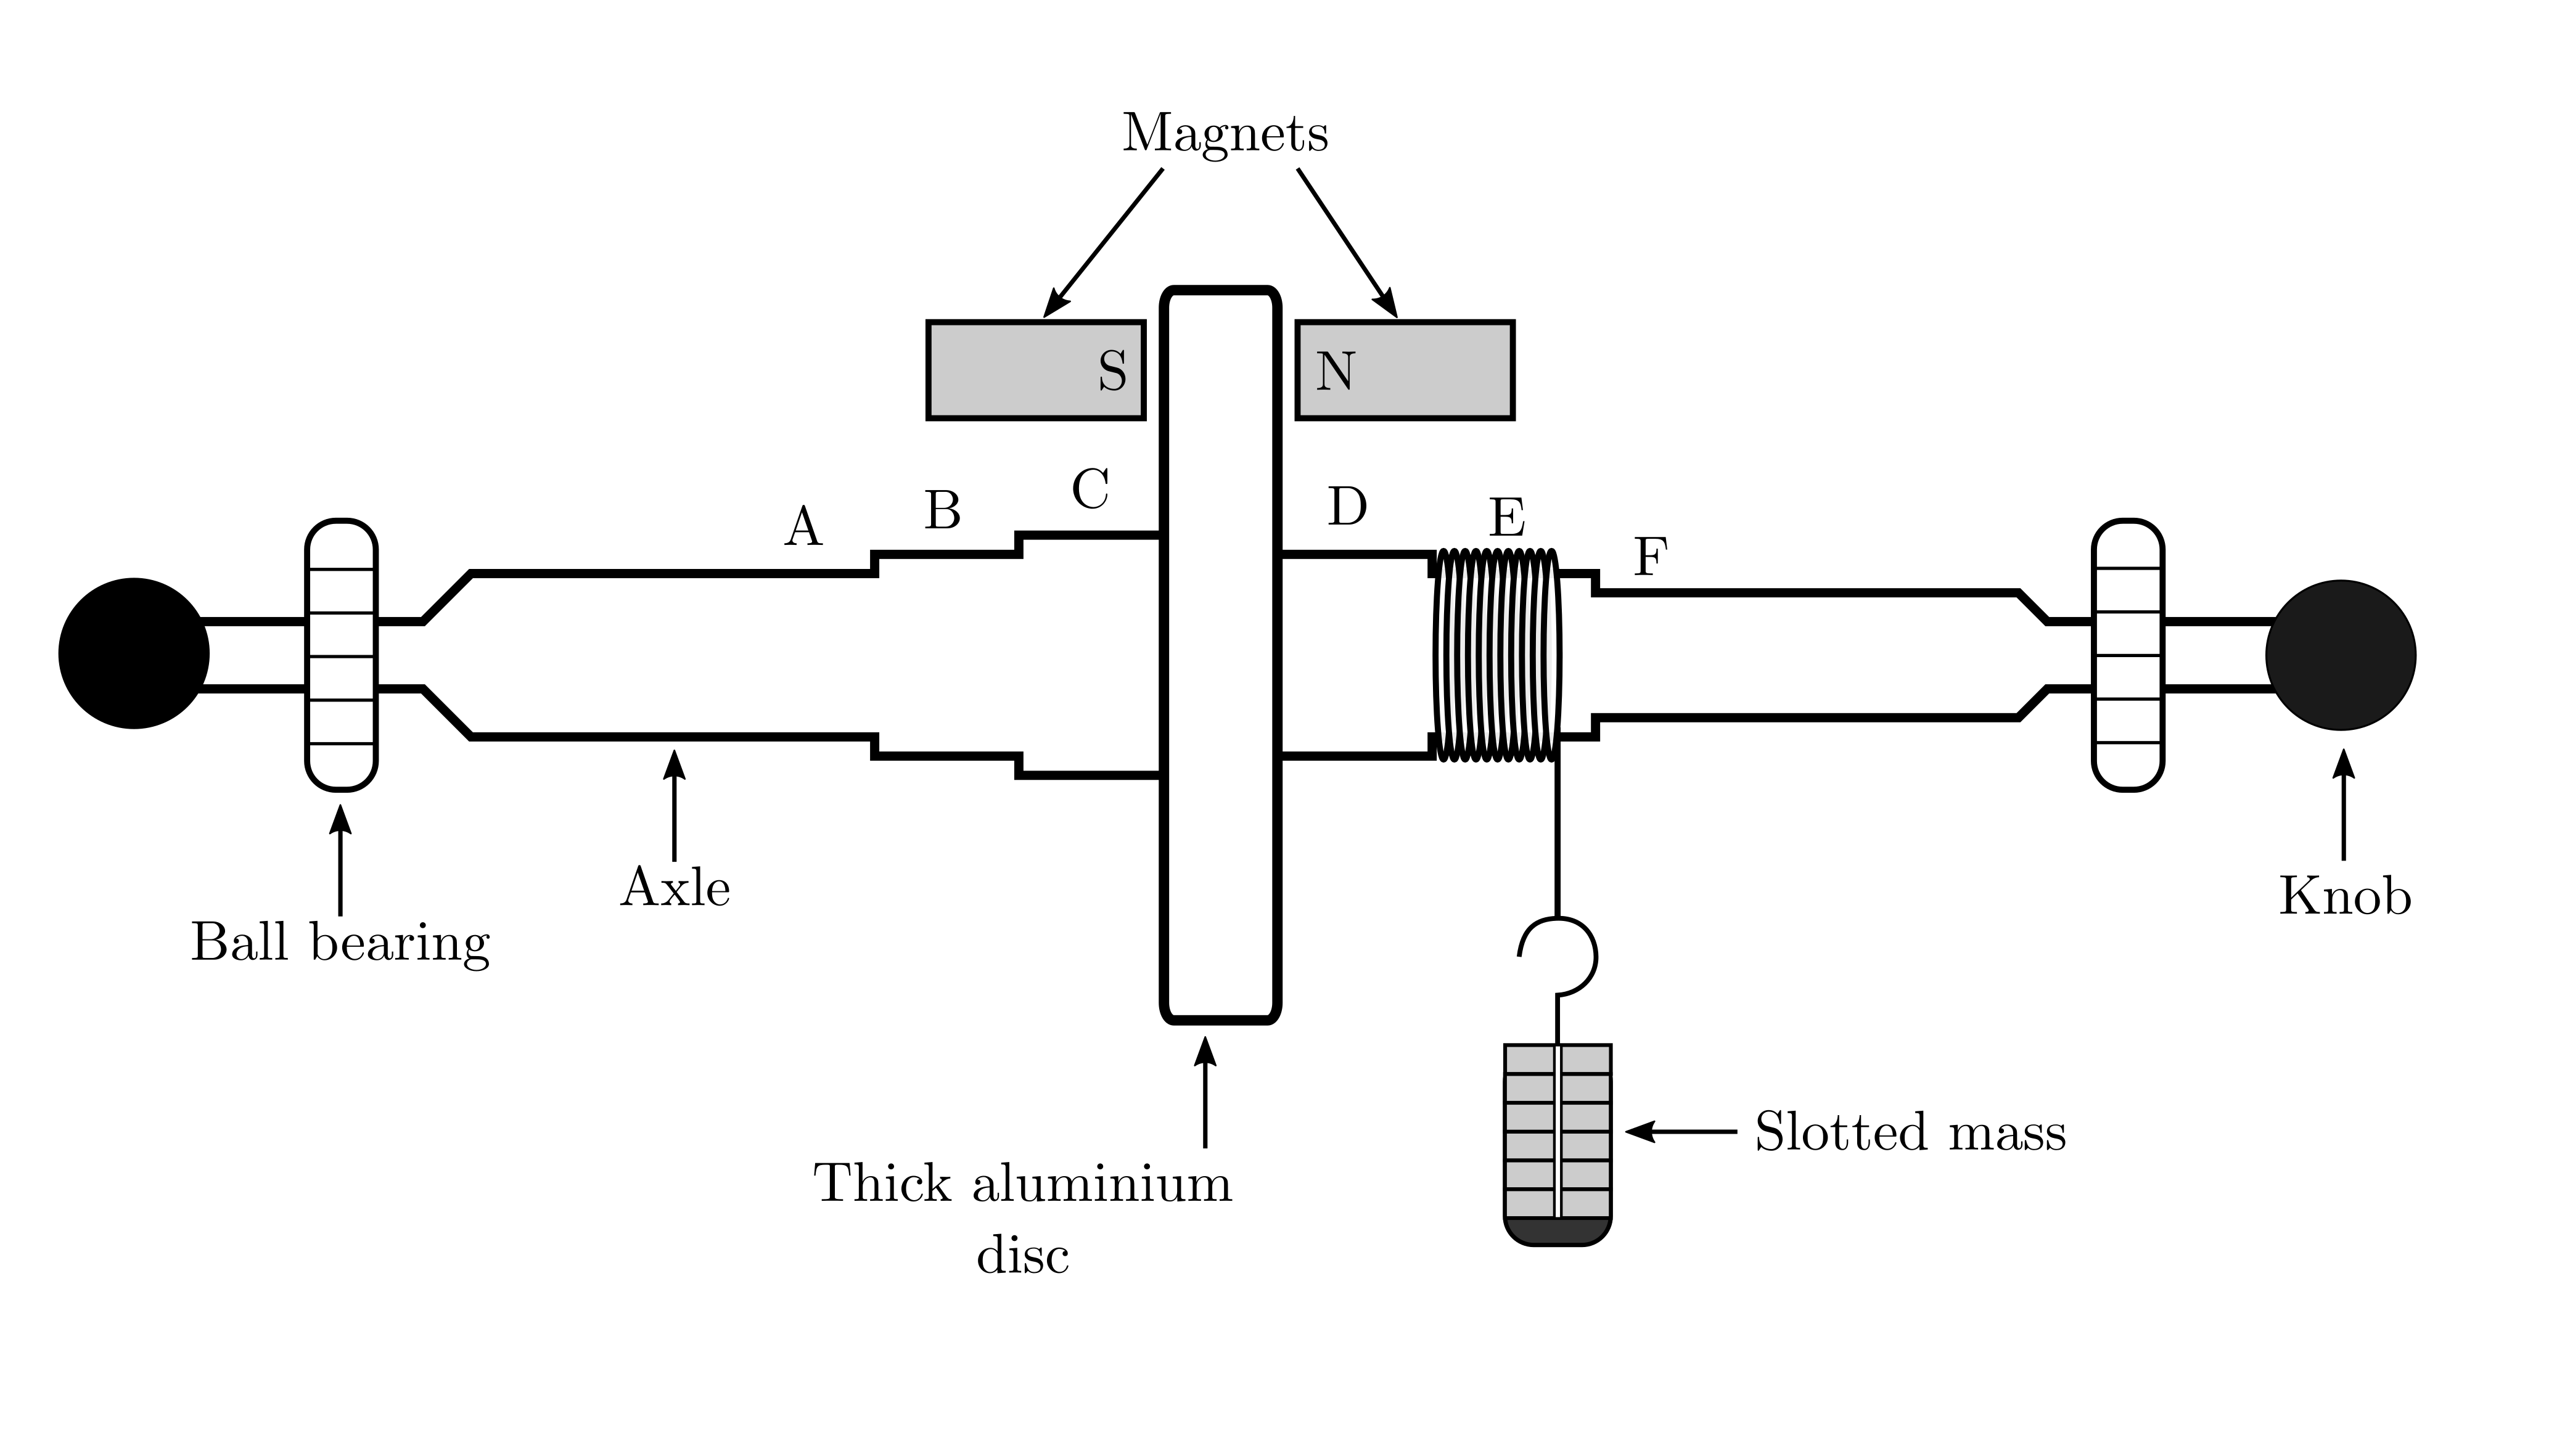
\includegraphics[width=\textwidth]{figs/em-damping/emdamping-setup.png}
    \caption{Schematic of the disc and magnet assembly. The different axles ($A$--$F$) are distinguished by their radii. The two magnets are placed on either side of the disc. The disc eventually rotates at a constant angular velocity because of the damping force due to the magnets. As a result, the slotted mass begins to fall with a constant terminal velocity.}
    \label{fig:emdamping-setup}
\end{figure}


\section*{Theory}

For rotating objects, Newton's Second Law may be generalised to 
\begin{equation}
    \tau = I \alpha
\end{equation}

where $\tau$ is the net external torque on the object, $I$ its moment of inertia, and $\alpha$ the angular acceleration. As the mass begins to fall, it will to accelerate, spinning the disk. It experiences two forces: gravity and the tension $T$ from the string, and thus accelerates at a rate $a<g$,
\begin{equation}
    ma = mg - T \quad \implies \quad T = m (g-a).
    \label{eqn:tension}
\end{equation}

\begin{figure}[!htb]
    \centering
    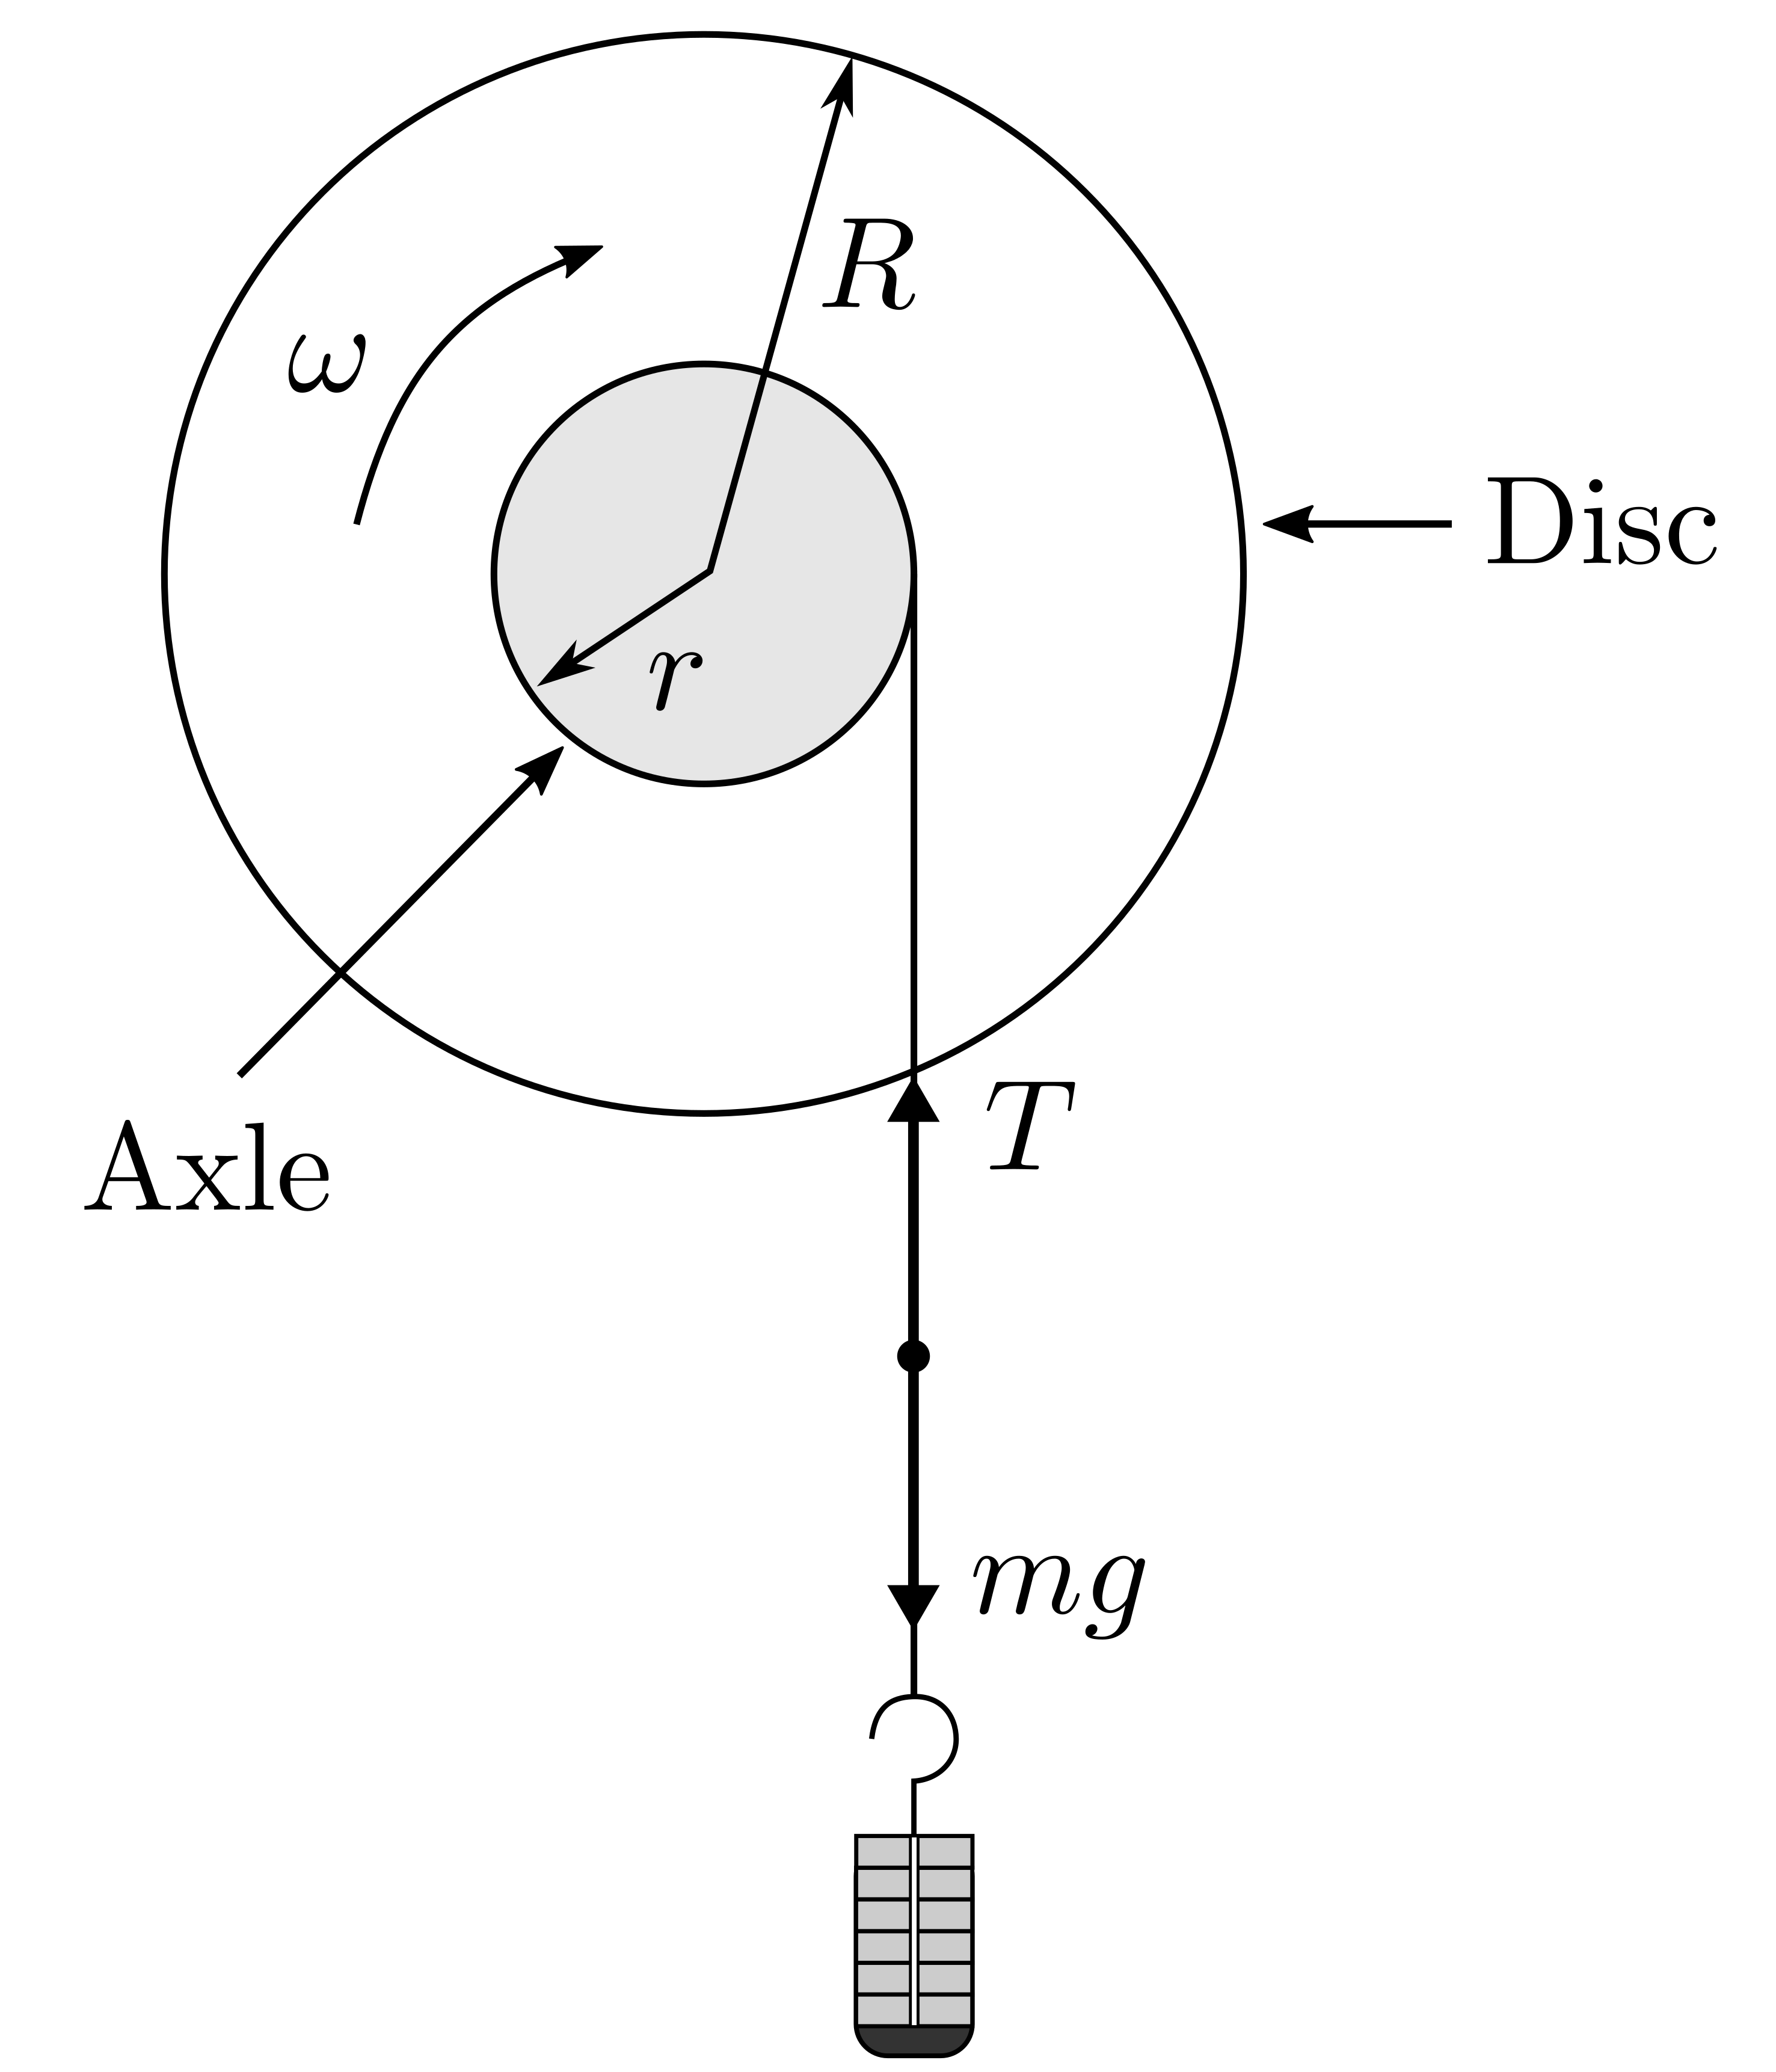
\includegraphics[width=0.4\textwidth]{figs/em-damping/emdamping-torque.png}
    \caption{View of the flywheel assembly from the side. The falling mass $m$ rotates the axle of radius $r$, which in turn causes the disc of radius $R$ to accelerate. Once the mass reaches terminal velocity due to electromagnetic damping, the disc moves at a constant angular velocity $\omega$. }
    \label{fig:emdamping-torque}
\end{figure}

Suppose the cord is wound around an axle of radius $r$. This means that the acceleration at the rim of the axle (i.e.\ at radius $r$) is the same as the acceleration of the mass. Thus
\begin{equation}
    \alpha = \frac{a}{r}
    \label{eqn:angularacc}
\end{equation}

\begin{question}
\textbf{Question:} The above situation is highly idealised, as it does not take into account friction. In practice, the disk will also experience a ``frictional'' torque $\tau_f$ which opposes its motion. Show, by balancing the torques on an axle of radius $r$, that 
\begin{equation}
    I \alpha = T r - \tau_f.
\end{equation}
\textbf{Question:} Using the equations for tension and angular acceleration (Equations~(\ref{eqn:tension}) and~(\ref{eqn:angularacc}) respectively) show that 
\begin{equation}
    a = g \left( \frac{m r^2}{I + mr^2}\right) - \left( \frac{r \tau_f}{I + mr^2}\right).
    \label{eqn:acc}
\end{equation}
\end{question}

\subsection*{Introducing damping}

The predominant damping in this set-up is due to electromagnetic damping. To understand how this occurs, let us focus on the electrons in the disc, which can move freely because the disc is a conductor. When an electron passes through the magnetic field, it experiences a Lorentz force $\vb{F} = e \vb{v} \times \vb{B}$. In this set-up, if we consider a point between the pole-pieces of the magnet, the magnetic field is perpendicular to the disc and the velocity of the electron is along the azimuthal direction. Thus the Lorentz force is along the radial direction. This force, acting on the electrons, causes them to systematically move in the radial direction. If the electrons were all pushed radially and could pile up at either the axle or the rim, an electric field would develop, which would grow until its effect exactly counteracted that of the magnetic field. But what we have here is a conductor that extends outward from the immediate vicinity of the pole pieces. Thus, the electrons moved by the Lorentz return to their original positions by a more circuitous route; closed, spread out currents are set up. Some of these eddy currents flow through the region between the pole pieces, and some of them flowing outside that region. 

Now let us focus on the current as it moves through the pole pieces. In these currents the charges move radially. A charge moving radially through the magnetic field experiences a force in the azimuthal direction. Note the three-step process: first, because the rotating conductor was carrying along the electrons with it, they were moving azimuthally, resulting in a radial Lorentz force; second, this radial Lorentz force causes a radial current, giving a radial component to the velocity of the electrons, and causing a current; third, the radially moving electrons in the current experience a Lorentz force in the azimuthal direction.

The question now arises: in which azimuthal direction does the Lorentz force on the radial current act? The direction can be established by carefully examining the direction of the field etc, but it can also be established from a more general principle. The azimuthal force must act such it it either helps the motion of the disk or hinders it. Suppose that the force acted such as to help the motion; then, a little push or fluctuation would start the process, and, with the help of the additional Lorentz force, would cause the wheel to turn faster, leading to a runaway situation that violates the conservation of energy. Thus the only possibility that can be realised in Nature is that the Lorentz force acts such as to hinder the motion of the wheel; it is a \textsl{damping} force.

Thus, the full torque balance on the disc is given by
\begin{equation}
    I \alpha = T r - \tau_f - \tau_B,
\end{equation}

where $\tau_B$ is the opposing magnetic torque that these currents produce. We will now try to calculate $\tau_B$ with an extremely simplified model.

\subsection*{Calculating the magnetic torque}

\begin{figure}[!htb]
    \centering
    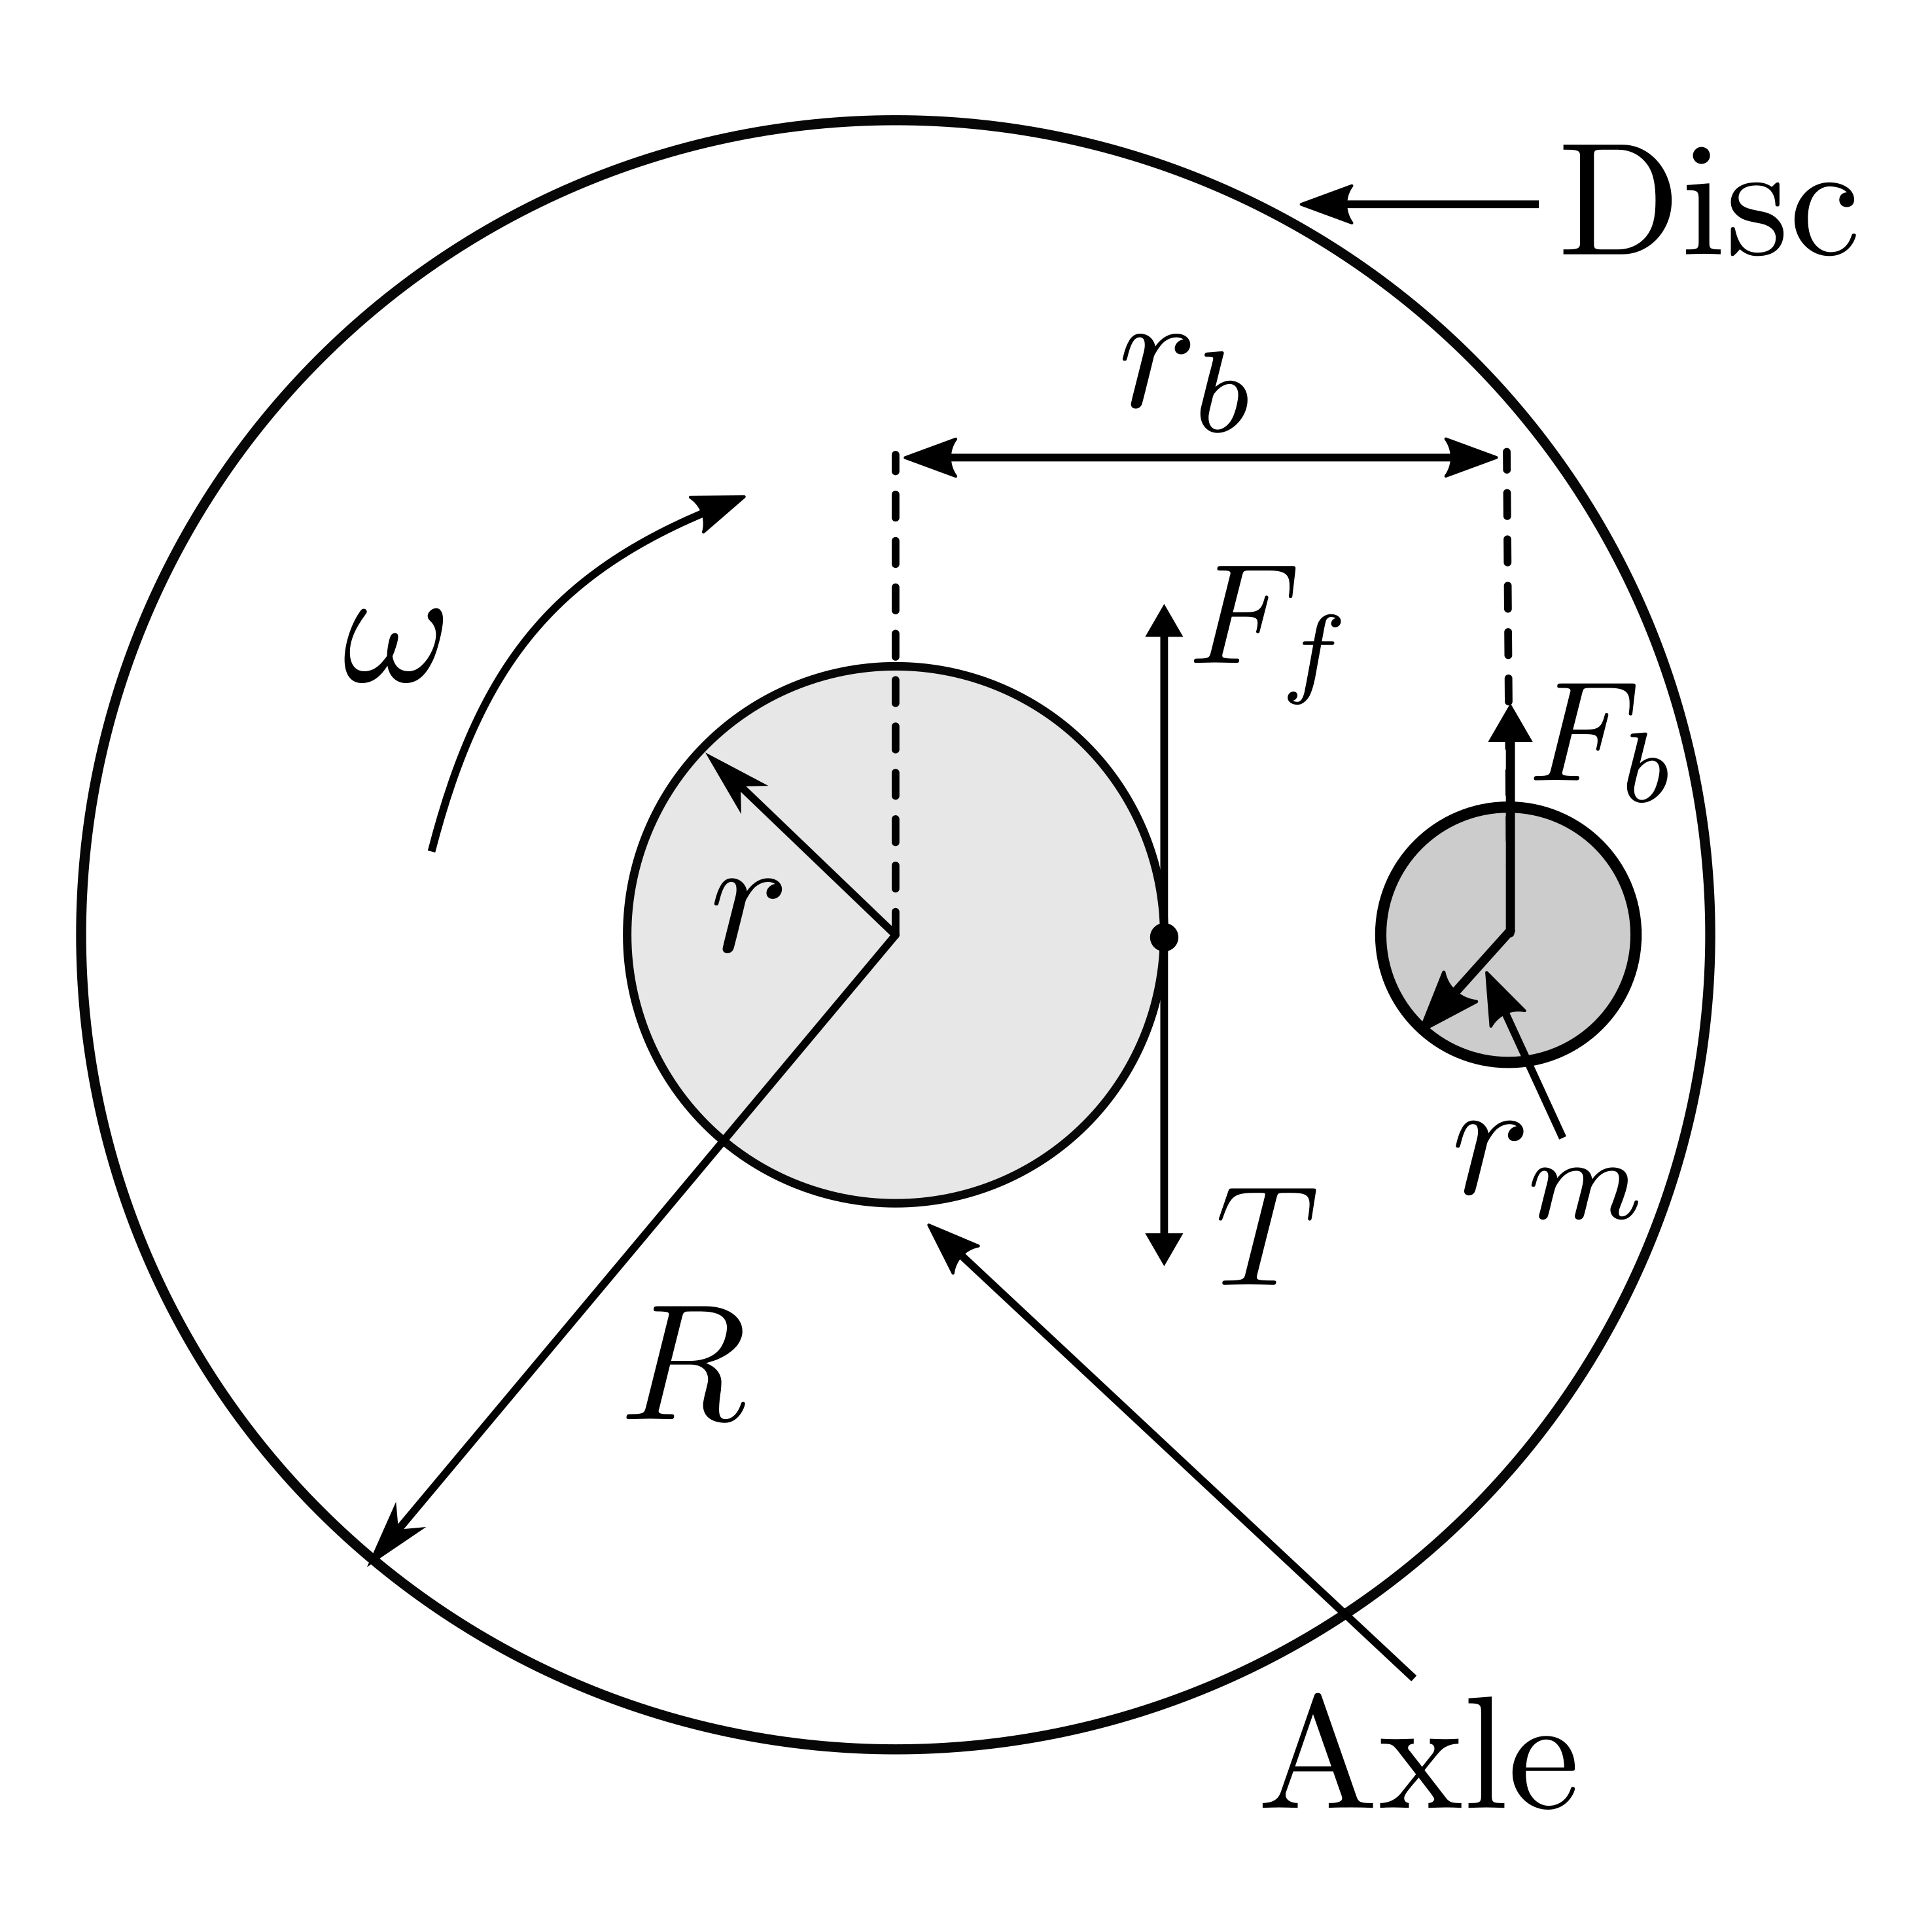
\includegraphics[width=0.4\textwidth]{figs/em-damping/emdamping-forces.png}
    \caption{View of the set-up from the side. The axle of the disc experiences a frictional force $F_f$ and the tension $T$ due to the string. A circular region of radius $r_m$, at a distance $r_b$ from the axle, experiences a damping force due to a nearly uniform $B$.}
    \label{fig:emdamping-forces}
\end{figure}

The magnetic field is confined to a small circular region $r_m \ll R$, the radius of the disc, as shown in Figure~(\ref{fig:emdamping-forces}), and is uniform over this region. Let us now consider a thin conducting path along the diameter of this region, of length $2 r_m$. It moves at a velocity $v = r_b \omega$, where $r_b$ is the distance from the centre of the circular region to the axis of rotation.

The emf $E_b$ induced is given by
\begin{equation}
    \mathcal{E}_b = (r_b \omega)\times B \times (2r_m).
\end{equation}

This emf $\mathcal{E}_b$ will give rise to a current $i$ (the eddy current) in a closed conducting path within the disc. Let us assume that this path has some resistance $R^*$.\footnote{This is a huge simplification: the reason eddy currents are so hard to model is because there are many different paths within the conductor of varying resistances.} Thus, the current is given by
\begin{equation}
    i = \frac{\mathcal{E}_b}{R^*} = \frac{(r_b \omega)\times B \times (2r_m)}{R^*}.
\end{equation}

These currents will in turn experience a force $F_b$ given by
\begin{equation}
    F_b = B i (2 r_m) = \frac{4 r_m^2 (\omega) r_b B^2}{R^*} = \left( \frac{4 r_m^2 r_b}{R^*}\right) \omega B^2.
\end{equation}

This force is responsible for the magnetic torque at $r$, $\tau_B$,
\begin{equation}
    \tau_B = r_b F_b = \left(\frac{4 r_m^2 r_b^2}{R^*} \right) \omega B^2 = C' \omega B^2.
\end{equation}

Now, in this derivation, we considered a conducting path going through the circular region of radius $r_m$. However, not all paths will have this length or even be radially directed. The effect of taking all these paths into consideration would be to given an average factor $C$ instead of $C'$. However, the dependence on $\omega$ and $B$ will remain unchanged. Thus, we can write the total torque as 
\begin{equation}
    I\alpha = m (g-a) r - \tau_f - C \omega B^2.
\end{equation}
As the retarding torque depends proportionately on the angular velocity of the disc, the disc will begin to slow until a steady state is obtained, i.e.\ until $\omega$ reaches some constant ``terminal'' value $\omega_t$. As a result, the mass will drop at some constant terminal velocity $v_t$. In this case, $\alpha=0$ and $a = 0$. 

\begin{question}
\textbf{Question:} Show that 
\begin{equation}
    v_t = \omega_t r = \left( \frac{g r^2}{CB^2}\right)\left( m - \frac{\tau_f}{g r}\right).
    \label{eqn:em-terminal}
\end{equation}
\end{question}

In this experiment, we will study the terminal velocity of the falling mass and its dependence on the mass and magnetic field.
 
\section*{Experimental Setup}


\subsection*{Apparatus}

\begin{enumerate}
\itemsep0em
\item A flywheel disc assembly, mounted on the wall
\item Two pairs of magnets with different pole strengths
\item A Gauss meter to measure magnetic fields
\item A set of slotted masses
\item A set of acrylic plates of different thicknesses
\item Metre scales and tapes
\item A spirit level
\end{enumerate}



% \subsection*{Description}


\subsection*{Precautions}
\begin{itemize}
\itemsep0em
\item Make sure the mass falls vertically, without horizontal oscillations.
\item The knobs on either end of the disc should be used to wind or unwind the cord.
\item Wind the cord on the axle carefully, so that the turns do not cross or overlap. Successive turns should touch each other, and should not extend beyond the length or diameter of the axle.
\end{itemize}



\section*{Procedure}

\subsection*{Part A}

You will begin this experiment by verifying Equation~(\ref{eqn:acc}) for the acceleration of the falling mass in the absence of a magnetic field. You will then use it determine the moment of inertia of the flywheel.

\begin{enumerate}
    \item Choose an appropriate axle and measure its diameter and note it down. Choose an appropriate length of cord and attach it to the axle.
    
    \item Attach the cord to a small slotted mass, and wind it carefully on the axle.
    
    \item Allow the mass to drop gently, taking care that it does not oscillate as it falls.
    
    \item Use a camera to take a video of the falling mass and analyse it to find its acceleration. You can use \textsl{Tracker} to obtain the position of the mass at different instants of time in the video.
    
    \item Once you have analysed your data for one video, repeat this procedure for different masses. 
    
    \item Plot an appropriate graph between the $a$ and $m$, and calculate the moment of inertia and frictional torque of the disc.
    
    % \begin{question}
    % \textbf{Question:} You will find that you have to plot a graph of the form
    % \begin{equation*}
    %     y = \frac{\alpha x}{\beta + x}
    % \end{equation*}
    
    % Show that by making a substitution $Y = 1/y$ and $X = 1/x$, you can reduce this graph to a linear graph
    
    % \begin{equation}
    %     Y = m X + C
    % \end{equation}
    
    % What are $m$ and $C$ in terms of $\alpha$ and $\beta$?
    % \end{question}
    \vspace{\parskip}
    \begin{question}
    \textbf{Question:} You will find that you have to plot a graph of the form
    \begin{equation*}
        a =  g \left( \frac{m r^2}{I + mr^2}\right) - \left( \frac{\tau_f r}{I + mr^2}\right)
    \end{equation*}
    
    Show, using an appropriate approximation, that this relation reduces to:
    
    \begin{equation}
        a \approx m \left( \frac{g r^2}{I}\right) - \left( \frac{\tau_f r}{I}\right).
    \end{equation}
    
    How would you find $I$ and $\tau_f$?
    \end{question}
    
\end{enumerate}

% \begin{question}
% \textbf{Question:} Would y-intercept would you expect this graph to have?
% \begin{enumerate}
%     \item Positive
%     \item Zero
%     \item Negative
% \end{enumerate}

% What do you think is responsible for this intercept?
% \end{question}

\subsection*{Part B}

Next, you will introduce electromagnetic damping to this system, which will make the mass fall at a terminal velocity $v_t$.
\begin{enumerate}
    \item Insert a pair of magnets in their holders, and place them on the assembly.
    
    \item Make sure that the magnets are equally spaced from the disc. In order to do this, bring them as close to the disc as possible, and note down the readings on the screw gauges on either side. Using this as your reference, rotate the screw gauge by the same amount on either side.
    
    \item Repeat the procedure given in \textbf{Part A}. In this case, the disc should finish by rotating at a constant angular velocity due to the electromagnetic damping.
    
    \item Plot a graph between the terminal velocity and the mass of the object, and show that it satisfies the relation for the terminal velocity given in Equation~(\ref{eqn:em-terminal}).
    
\end{enumerate}

\subsection*{Part C}

Finally, you will vary the strength of the magnetic field and measure how the terminal velocity $v_t$ varies with the external magnetic field $B$.
\begin{enumerate}
    \item Vary the distances between the magnets and measure the magnetic field $B$ exactly between the magnets using a Gauss meter. Plot a graph of $B$ as you vary the magnets' separation. This graph will tell you what the magnetic field should be at the centre of the disk as you vary the separation between the magnets.
    
    \item Next, keep the magnets some known distance apart and measure $v_t$ for a fixed value of mass. 
    
    \item Without changing any of the parameters in the system (including the mass), change the separation between the magnets (effectively varying $B$) and calculate the $v_t$. Repeat this for different separations between the magnets. Find how the terminal velocity $v_t$ varies with $B$.
    
\end{enumerate}
\chapter{Equipotential Curves}

\section*{Objectives}
\begin{enumerate}
\item To understand the relationship between electric fields and voltages.
\item To study the properties of electric fields in two-dimensions by mapping equipotential curves and constructing the corresponding lines of force.
\end{enumerate}


\section*{Introduction}

You may remember from school that any configuration of static electric charges produces an electric field in space. Such an electric field is a vector quantity that is a function of position, meaning that it has both a magnitude and direction at every point in space. Consider, for example, a point charge $q$ at the origin, whose electric field is well known from Coulomb's law,
\begin{equation}
    \vb{E} = \frac{1}{4\pi \epsilon_0} \frac{q}{r^2} \hat{\vb{r}}.
\end{equation}

The above equation tells us that the electric field vectors point radially outward\footnote{Or inward, if the charge is negative.} from the charge and that their magnitudes fall off as the reciprocal of the square of the distance from it.

When one has a collection of several charges, the electric field obeys the principle of superposition. In other words, the resulting electric field is the vector sum of all the contributions of the individual parts. This makes it possible to (theoretically) calculate the field produced by any collection of charges. Practically, however, this is very hard to do even for simple charge configurations, because of the vector nature of the field. This also results in the electric field being difficult to grasp or visualise. There is, however, a very simple way to arrive at this vector field, using a concept known as the \textsl{electric potential} $V$.

\section*{Theory}

\subsection*{Electric fields and potentials}

Maxwell's equations completely describe a static electric field through its divergence and curl
\begin{equation}
    \begin{aligned}
        \div{\vb{E}} &= \rho/\epsilon_0,\\
        \curl{\vb{E}}&= \vb{0},
    \end{aligned}
\end{equation}

where $\rho$ is the charge density and $\epsilon_0$ a constant known as the permittivity of free space.

\begin{question}
\textbf{Question:} Using the second equation above, show that this implies that every static electric field can be expressed as the gradient of a \textsl{scalar} field, called the electric potential $V$. In other words, show that 
\begin{equation}
    \vb{E} = - \gradient{V}
\end{equation}
\end{question}

If no net charge accumulates in a region, we can say that the charge density $\rho = 0$ in this region. In this case, the potential satisfies \textsl{Laplace's Equation}:
\begin{equation}
    \laplacian{V} = 0.
    \label{eqn:laplace}
\end{equation}

Being a scalar, $V$ just requires a single number at every point, which makes it much easier to work with. We can obtain the electric field from the potential by taking its \textsl{gradient}. The gradient of a scalar function is a vector whose $x$, $y$, and $z$ components are the rate at which the function changes along $x$, $y$, and $z$, respectively. A consequence of this is that the gradient vector, at any position, points along the direction in which function changes fastest and its magnitude is the rate of change of the function along this direction. Thus, the potential contains all the information that the field does.

Here is a simple way to visualise this: imagine connecting the points at which the potential has the same value. This is rather like connecting the points on a hill that are at the same height.\footnote{Or rather, same ``gravitational'' potential!} If this is done for a series of equally spaced values, what results is a contour map, with each contour representing a single value of the height. In the case of electric potential, these contours are called equipotential curves.\footnote{In general, in three dimensions, the points which have the same potential lie on a two-dimensional surface, known as an equipotential surface.} It is easy to see that where the contours are closely spaced the potential changes rapidly and where they are widely spaced the potential changes slowly in space. Given how the potential is defined (as a gradient), it should be easy to see that the magnitude of the electric field is larger in the first case than in the second case. Another important rule about these contour lines and the electric field is that field lines always meet contour lines at right angles. This is because the $\vb{E}$ field always points in the direction where $V$ is changing the most rapidly. It makes sense, then, that the direction perpendicular to the $\vb{E}$ field is the direction where $V$ is not changing at all. Since this direction must be along the equipotential surface by definition, the electric field is locally perpendicular to the equipotential surface.

\begin{question}
\textbf{Question:} What are the equipotential surfaces for the point charge we discussed earlier? Consider three equipotential surfaces that are equally spaced in potential. Are they spaced equally \textsl{in space}? If yes, why? If not, how do they change? How would this change if the charge was negative instead of positive?

\textbf{Question:} Now imagine an infinite wire of charge lying along the $x$-axis. What would the equipotential surfaces be in this case?
\end{question}

\subsection*{Conductors as equipotential surfaces}

A conductor is a material with the property that the charge in it is free to move around. A material which does not have this property (i.e.\ one in which the charges are stationary) is called an insulator. In practice, almost all metals are good conductors and most other substances are insulators. In static equilibrium has the property that the electric field is zero everywhere inside. The reason is simple: if it weren't zero somewhere, the charge there would move in the direction of the field, so it wouldn't be in static equilibrium. One important consequence of this is that all points within a conductor are at the same potential. This is because a difference in potential would imply an electric field, which would push the electrons in the conductor in such a way as to reduce the field; this continues until the electrons in the interior or the conductor are pushed to the surface. And, on the surface, they are moved around until the component of the field along it vanishes. Thus, the surface of a conductor is an equipotential surface.

\begin{imp}
Suppose now you have a region of space enclosed by two equipotential surfaces (say, the region between two concentric spheres), and you are interested in the potential at all points between them. We can compute the potential at every point in this region of space by solving Laplace's Equation (Equation~(\ref{eqn:laplace})) with the appropriate value at the boundaries. We can then find the equipotential surfaces, since they are simply are the loci of points where this solution to Laplace's Equation has the same value.
\end{imp}

% \begin{imp}
% Be careful about applying these facts too generally: it's very easy to have a conductor which is not in static equilibrium! This is why conductors are usually used: to maintain a steady flow of charge, what we call a current, as you will learn in another experiment. A conductor which is carrying a current is not an equipotential; instead, the current flows from high to low potential inside the conductor.
% \end{imp}

Since the conductors we will be using are equipotential surfaces, we can find the potential in the region in between them by solving Laplace's Equation. This is, in general, a daunting task. However we can often use the symmetry of simple configurations to solve for $V$ easily.

\subsection*{Some interesting configurations}

In this experiment, you will be given some metal electrodes and asked to find the curves of constant potential. You will be asked routinely to solve such problems in electrostatics in the course on \textsl{Electricity and Magnetism} you have this semester. Let us try to do this for some simple configurations. We will be working in two dimensions of space (the surface of the water). 

\begin{figure}[!htb]
\captionsetup[subfigure]{justification=centering}
\centering
        \begin{subfigure}[b]{0.6\textwidth}
        \centering
                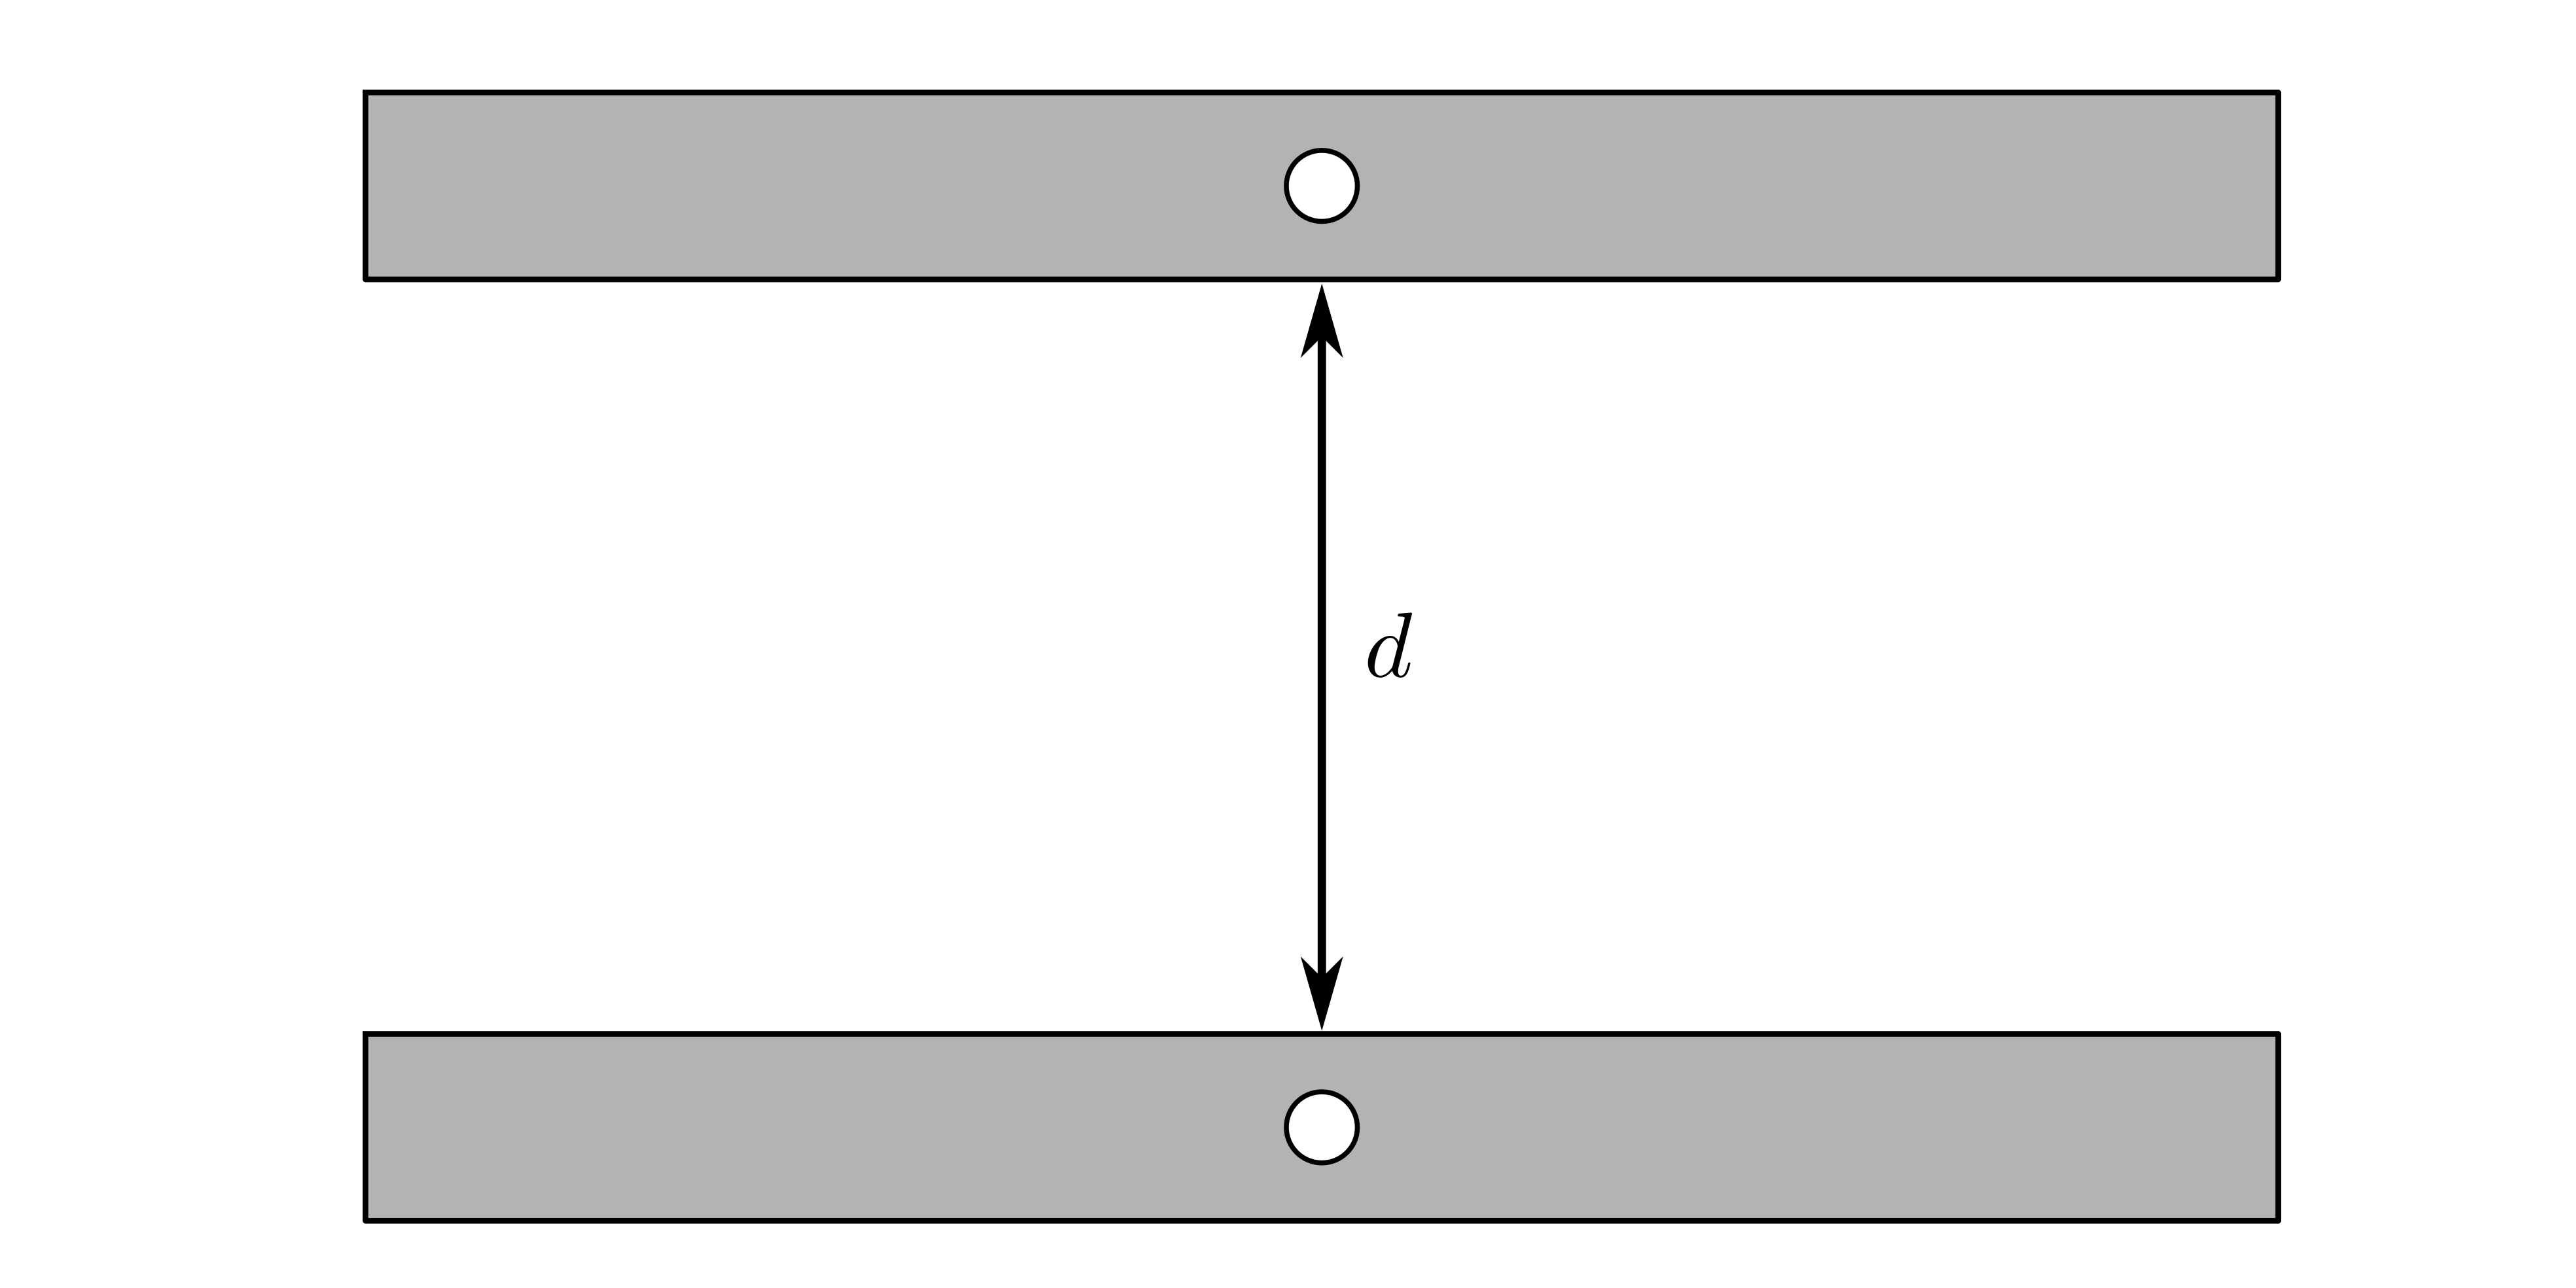
\includegraphics[scale=0.5]{figs/equipotential-curves/equipotential-parallel-plates.png}
                \caption{ ``Infinite" parallel bars}
                \label{fig:parallel-plates}
        \end{subfigure}\hfill
        \begin{subfigure}[b]{0.4\textwidth}
        \centering
                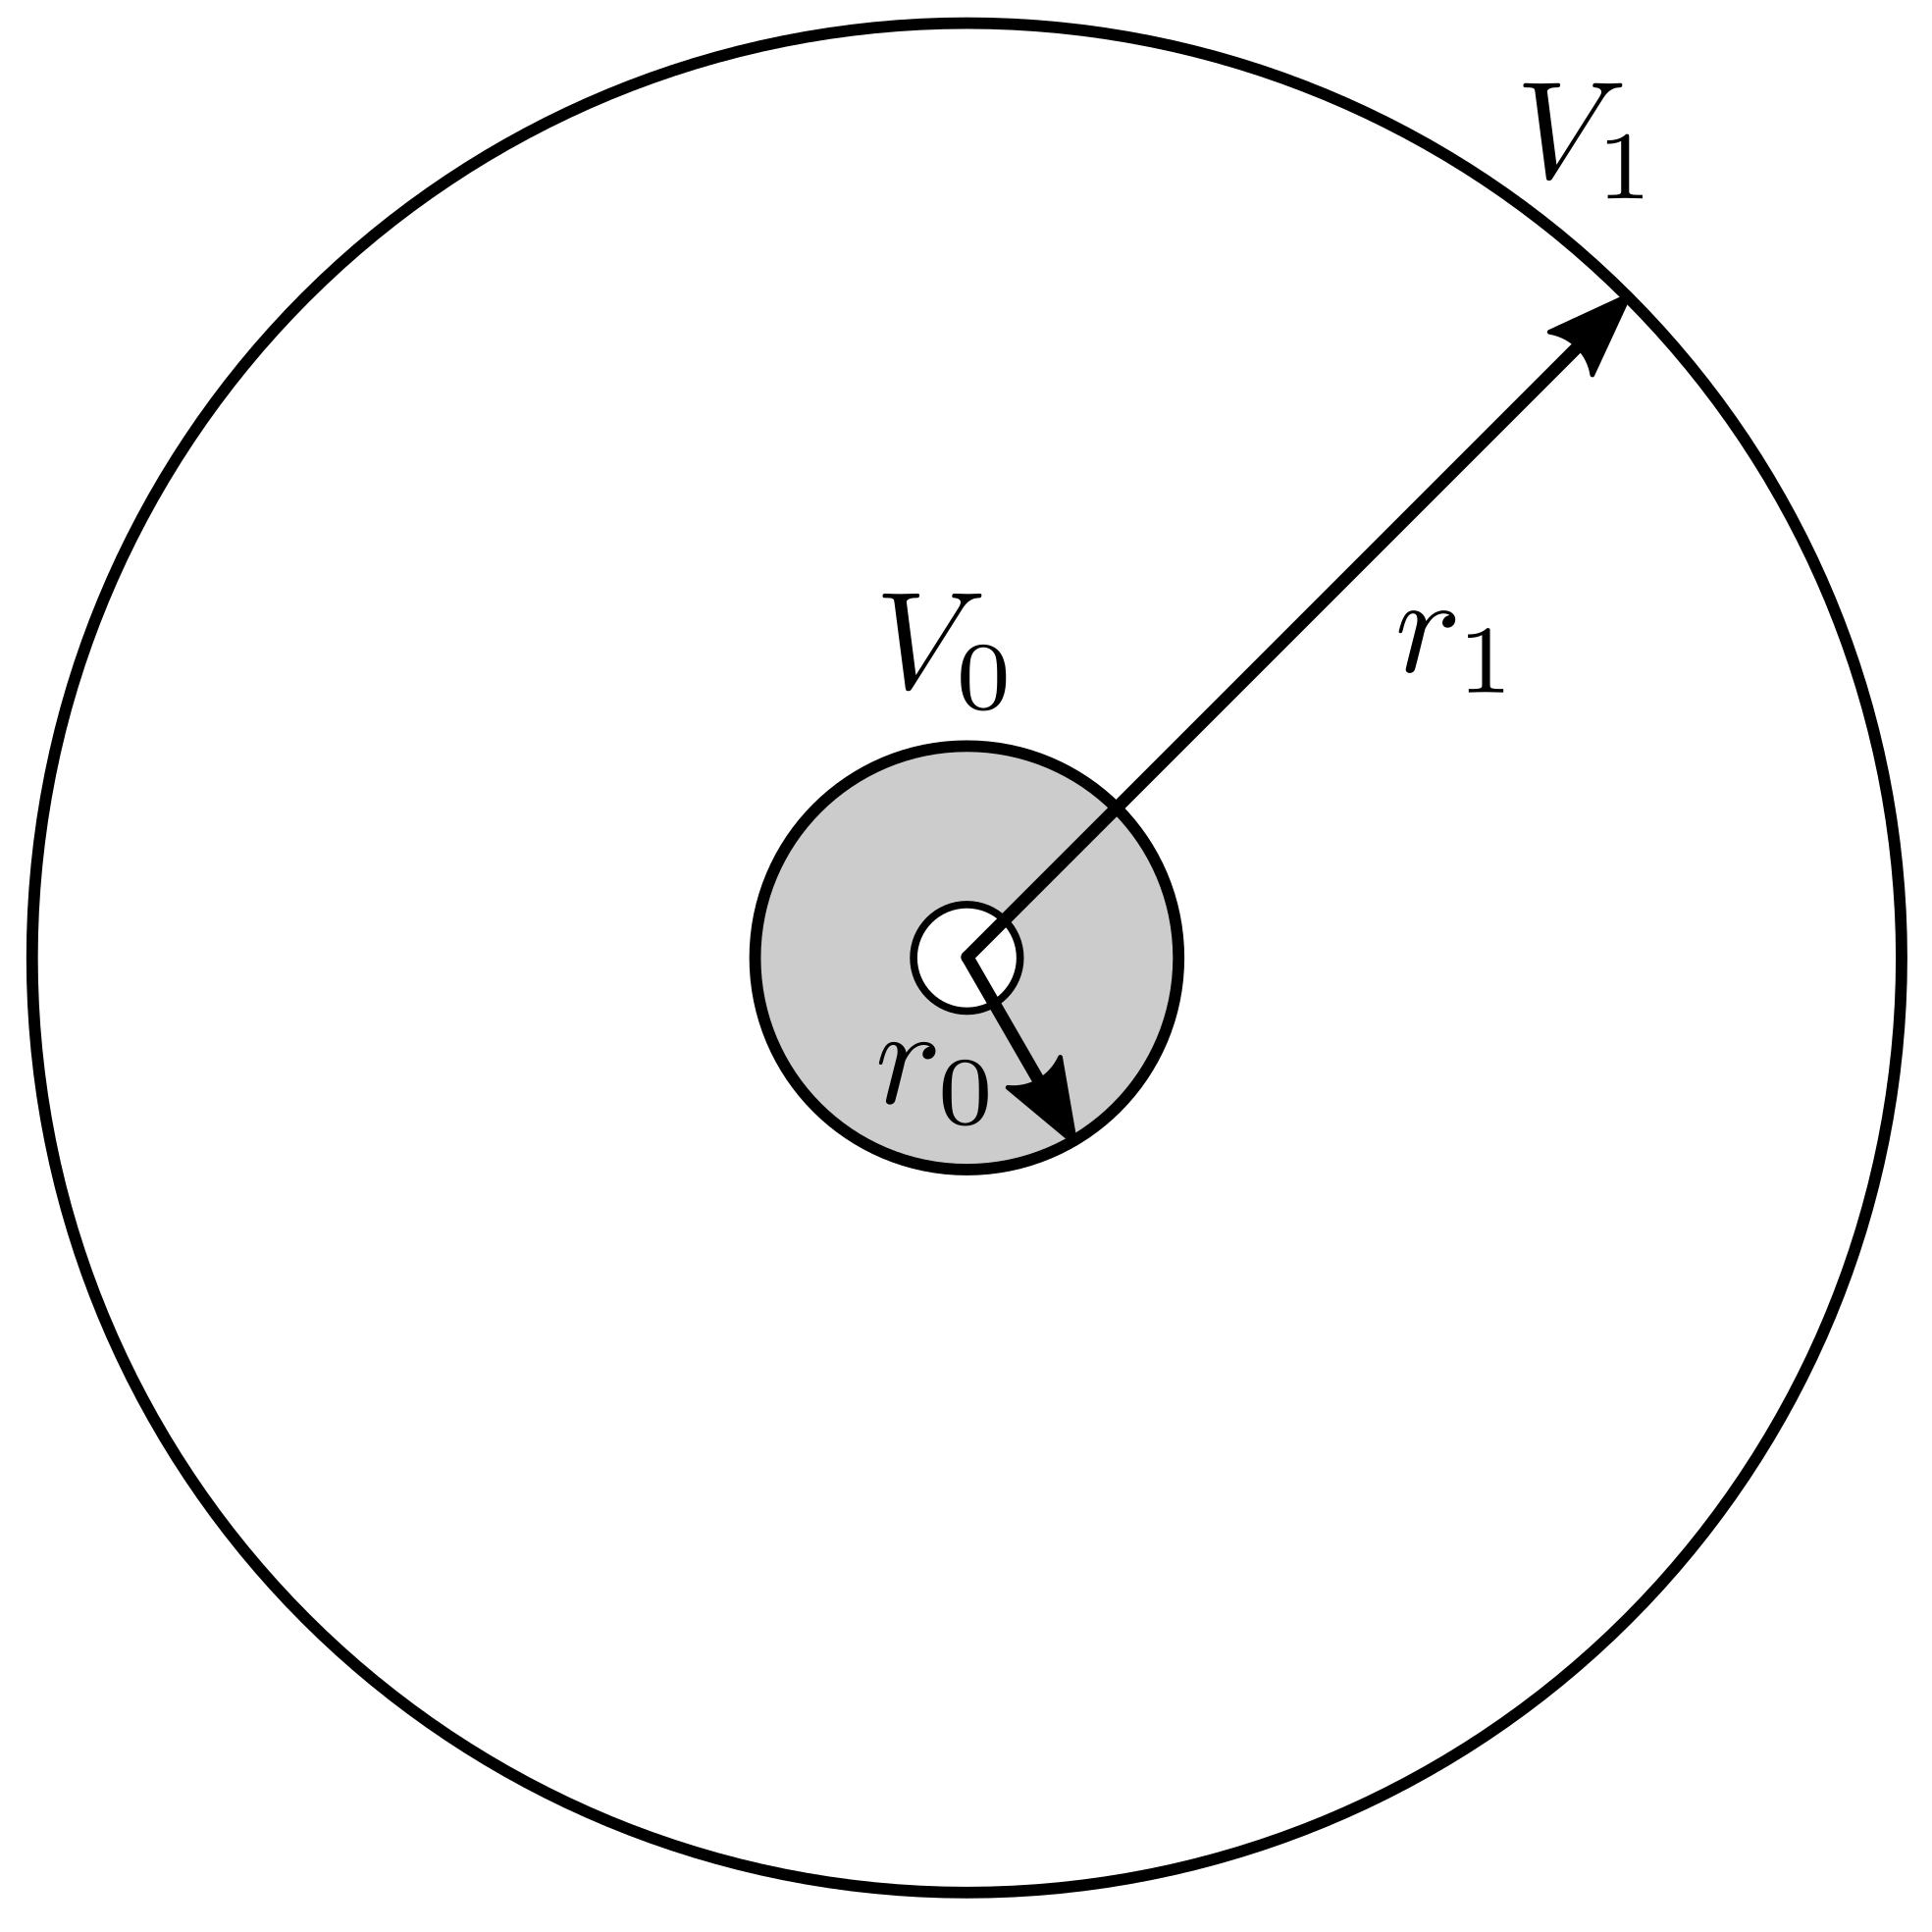
\includegraphics[scale=0.5]{figs/equipotential-curves/equipotential-concentric-cylinders.png}
                \caption{Concentric cylinders}
                \label{fig:concentric-cylinders}
        \end{subfigure}
        \caption{Two exactly solvable electrostatic configurations showing different symmetries.}
        \par\bigskip
\end{figure}


\subsubsection*{The parallel-bar ``capacitor''}

Consider first two parallel bars as shown in Figure~(\ref{fig:parallel-plates}), infinite in one direction and separated by some distance $d$ in the other. Laplace's equation can be written in Cartesian coordinates as
\begin{equation}
    \pdv[2]{V}{x}+\pdv[2]{V}{y} = 0.
\end{equation}

However, since the bars are infinitely long, it should be clear to you that there can be no variation in the potential along $x$ (as the plates are infinite, moving a finite distance to the right or left would not change anything). Thus, the equation reduces to 
\begin{equation}
    \dv[2]{V}{y}= 0.
\end{equation}

\begin{question}
\textbf{Question:} Suppose the top bar is at some potential $V_0$ and the other is grounded (i.e.\ at potential $0$), and they are both separated by some distance $d$. Show that the solution to this equation is
\begin{equation}
    V(y) = V_0 \times \left(\frac{y}{d}\right),
    \label{eqn:parallel-plate-field}
\end{equation}
where $y$ is the distance measured from the bottom bar.
\end{question}


\subsubsection{Two concentric cylinders}

Consider now that you have two concentric cylinders, as shown in Figure~(\ref{fig:concentric-cylinders}) The inner cylinder (of radius $r_0$) is at some potential $V_0$ and the outer cylinder (of radius $r_1$) is grounded. In this case, given the cylindrical symmetry of the problem, it is better to solve the problem in cylindrical coordinates. You can easily show that Laplace's equation can be written as 
\begin{equation}
    \frac{1}{r}\pdv{}{r}\left(r \pdv{V}{r}\right) + \frac{1}{r^2}\pdv[2]{V}{\theta} = 0.
\end{equation}

Just as before, we can ignore the $\theta$ term by symmetry (if we rotate the system by any angle, nothing seems to change). i.e.\ 
\begin{equation}
    \frac{1}{r}\dv{}{r}\left(r \dv{V}{r}\right) =0.
\end{equation}

\begin{question}
\textbf{Question:} Show in this case that Laplace's equation is satisfied by a function of the form
\begin{equation}
V(r) = a \ln\left(\frac{r}{r_0}\right) + b.
\end{equation}

\textbf{Question:} By using the fact that at $r = r_0$, the voltage is $V = V_0$, and when $r = r_1  \neq r_0$, the voltage is $V = V_1$, show that
\begin{equation}
    V(r) = \dfrac{(V_1 - V_0) \ln{\left(\dfrac{r}{r_0}\right)}}{\ln{\left(\dfrac{r_1}{r_0}\right)}}  + V_0.
    \label{eqn:concentric-cylinder-field}
\end{equation}

\end{question}

\section*{Experimental Setup}

\subsection*{Apparatus}

\begin{enumerate}[label=\arabic*)]
\itemsep0em
\item An acrylic tray with electrolytic medium (water)
\item An AC power supply with a voltage stabiliser 
\item A set of metallic electrodes
\item A digital multimeter
\item A pointed probe attached to an $XY-$stage
\item A set of connecting cords
\item A set of measuring scales
\end{enumerate}

 \subsection*{Description}

In this experiment you will study the electric potential produced by sets of metallic electrodes of different shapes and sizes, held at a fixed voltage. To plot the equipotential curves, the metallic electrodes are kept in an acrylic tray such that three-fourths of their height is submersed within an electrolyte (tap-water will do) which is used as an electrolytic tank. An AC potential difference is maintained between the electrodes, which causes a distribution of potential in the electrolyte. By measuring the potentials at different points, one can identify the coordinates of the points of equal potential and consequently plot the equipotential curves on a graph sheet. 

\begin{tip}
This experiment can be performed either with AC or DC voltage from the provided power supply. However, while using DC voltage, electrolysis is found to occur, and the aluminium electrodes begin to get eaten away. As a result, it is advisable to use AC voltage from the power supply.
\end{tip}

\subsection*{Precautions}

\begin{itemize}
\item Arrange the electrodes and keep them stable and undisturbed throughout the measurements. You can use some tape to keep them fixed.
\item Make sure the uninsulated tip of the measuring probe just grazes the surface of the water.
\item Both graph papers -- the one attached below the tray and the one used for noting your data -- should have same coordinates and precision in scale.
\end{itemize}


\section*{Procedure}

Begin by taking two graph sheets and drawing the same coordinate system on them. You will stick one of these sheets on the bottom of the acrylic tray and use it as a reference. You will then mark out the potentials at different points on the other sheet, using the first as a reference.

\subsection*{Part A} 

\begin{enumerate}
    \item Place the two long electrodes parallel to the $x$-axis symmetrically about the origin, as shown in Figure~(\ref{fig:parallel-plates}).
    
    \item A potential difference is established across the electrodes by connecting them to the AC power supply.
    
    \item Using the multimeter, test the potential difference between the electrodes in volts. If it is found to be significantly different from the value you are supplying, ask a TF or instructor for help. 
    
    \begin{question}
        \textbf{Question:} What should the equipotential surfaces look like in this case?
    \end{question}
    
    \item Using the same ground as a reference, connect the positive wire of the multimeter to the probe and qualitatively measure the change in the potential from one end of the acrylic tray to the other.
    
    \item Measure the voltage at an arbitrary point and then find multiple points with the same potential thus drawing out one of the equipotential curves. 
    
    \item Choosing an appropriate increment in voltage, find the equipotential curves for different values of the potential. Verify Equation~(\ref{eqn:parallel-plate-field}) in the appropriate limit. 
    
    \begin{question}
        \textbf{Question:} Do you see Equation~(\ref{eqn:parallel-plate-field}) being satisfied everywhere? What could be the reason for this?
    \end{question}


\end{enumerate}


\subsection*{Part B}

\begin{enumerate}
    \item Set up the electrodes as shown in Figure~(\ref{fig:concentric-cylinders}). Maintain the inner cylinder at a higher voltage $V_0$ and ground the outer cylinder.
    
    \begin{question}
        \textbf{Question:} What should the equipotential surfaces look like in this case?
    \end{question}
    
    \item As before, choose an appropriate increment in voltage and find the equipotential curves for different values of the potential. 
    
    \item Use this to verify the equation for the voltage between two concentric cylinders, given in Equation~(\ref{eqn:concentric-cylinder-field}).
\end{enumerate}



\subsection*{Part C}

Explore the equipotential curves for a single configuration of your choice. 

\begin{tip}
    You can visit following online applet: \nolinkurl{falstad.com/emstatic/} and play around with the various different configurations to see how the field lines and contour lines are produced by different distributions of charges. 
\end{tip}
\chapter{Electronic Circuits}

\section*{Objectives}

\begin{enumerate}
\item To study the response of an RC circuit as a low-pass Filter and a high-pass Filter.
\item To study the response of an LCR circuit in different configurations.
\end{enumerate}


\section*{Introduction}

When a potential difference is applied across a conductor, it causes a flow of electrons known as a \textsl{current}. An ideal conductor will be able to sustain such a current indefinitely without losing any energy. However, in realistic conductors, the amount of current that can flow is limited by a material property of the conductor known as the ``resistivity''. To model such realistic systems, in our simplified circuits we consider an electronic component known as a \textsl{resistor}. We imagine an ideal resistor constructed as shown in Figure~(\ref{fig:electronics-components}): two perfectly conducting wires attach to two ends of a ``bar'' of resistive material. In such an ideal resistor, it then follows that the applied voltage $V$ and the produced current $I$ are proportional to each other through a constant of proportionality known as the ``Resistance'' of the resistor $R$. Thus, we get what is commonly known as Ohm's law,
\begin{equation}
    V = I R.
    \label{eqn:ohms-law}
\end{equation}

In more advanced courses, you will see that this linear relationship between the current and the voltage is only approximate for real conducting materials. However, this approximation is more than sufficient for our purposes.


\begin{figure}[!htb]
    \centering
    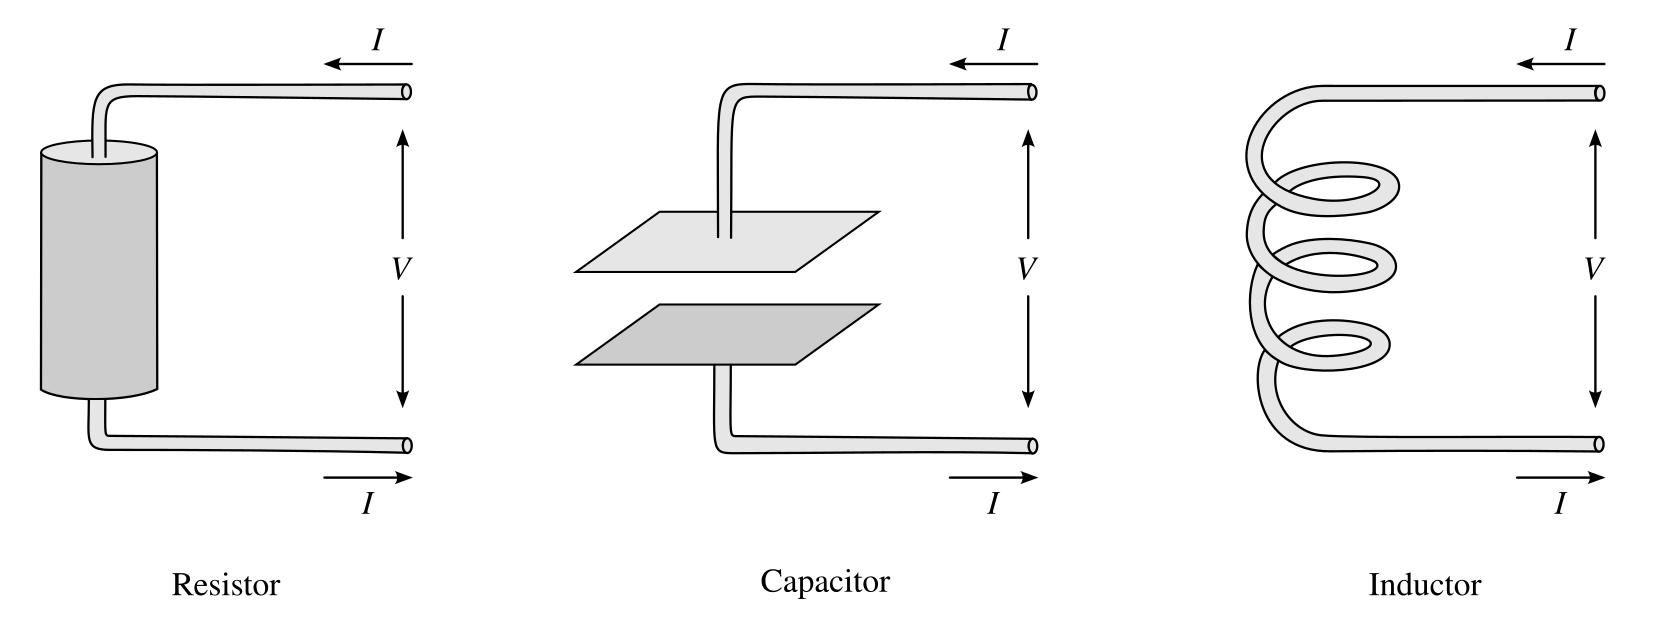
\includegraphics[width=\textwidth]{figs/electronics-circuits/electronics-components.png}
    \caption{Three passive circuit components. Resistors are conductors  }
    \label{fig:electronics-components}
\end{figure}



You should all be quite familiar with resistances by now. Figure~(\ref{fig:electronics-components}) also shows two other electronics components with which you are perhaps less familiar. The first of these is a ``capacitor''. As shown in the figure, a capacitor consists of two perfectly conducting wires attached independently to two perfectly conducting plates. When a constant voltage is applied across such a system, it causes a flow of current. However, since the two plates are not in contact with each other, the current simply leads to a build-up of charge on each of the capacitor's plates. The net charge in the system being constant implies that the upper plate accumulates a charge of $+Q$, while the lower accumulates a charge of $-Q$. It can be shown that the potential difference between the plates $V$ is proportional to this charge, and that 
\begin{equation}
    V = \frac{Q}{C},
    \label{eqn:def-cap}
\end{equation}

where $C$ is a constant for a capacitor, known as its ``capacitance''.

The last component is the inductor. An inductor is constructed by winding many turns of a perfectly conducting wire in the form of a coil, and bringing the two ends out to terminals at some distance from the coil. When a voltage $V$ is applied across such a system, it causes a current $I$ which produces a magnetic field as it flows through the loops. In an ideal inductor, we assume that the magnetic field remains contained within the coil. We further assume that in such an ideal system, the wire has no resistance, and that there is no build-up of charge on the surface of the wires. When a current passes through such a coil, a magnetic field proportional to the current is built up inside it. If the current changes as a function of time, this magnetic field also changes. From Lenz's law, you should recall that such a changing magnetic field induces an electromotive force which translates to an induced voltage. The voltage generated in this way can be shown to be 
\begin{equation}
    V = L \dv{I}{t},
    \label{eqn:def-ind}
\end{equation}

where $L$ is a constant for an inductor, known as its ``inductance''.

The way we have described the above components illustrates a general approach that we will take in analysing circuits: the properties of these components are described completely in terms of the currents and voltages that are measured at the \textsl{terminals}. This allows us -- provided certain simplifying assumptions are made -- to ignore the great complexities of the inner workings of these components.

In the description of the inductor given above, you should be able to see that it behaves differently depending on the type of current passed through the circuit. If a constant current flows through an inductor, it essentially behaves like an ideal conducting wire. However, if instead we provide a time-varying current, a potential drop will be observed across the inductor, by an amount proportional to its inductance $L$. Thus, we see that our circuit components need not behave in the same way when exposed to constant ``direct'' current (DC) or ``alternating'' current (AC).

In fact, it is much more general than this. As we shall see, certain circuit elements like inductors and capacitors exhibit a \textsl{frequency} response, meaning that they behave differently when different frequencies of AC are passed through them. This is precisely what you will be studying throughout this experiment.


\section*{Theory}

We will now motivate the basic responses of resistors, capacitors, and inductors to alternating current. Keep in mind that unless explicitly stated, we will be assuming that our circuit components are all \textsl{ideal}. In reality, this is of course an approximation, but one that is valid in our experimental conditions.

One of the consequences of assuming ideal components is that we will be dealing with \textsl{linear} systems. You will see such systems appear throughout your physics curriculum, which is why they are so important to study. As we shall see, the mathematics of our simple electrical systems maps perfectly onto the mathematics of simple mechanical systems, meaning that all of our electrical systems have mechanical analogues. 

Additionally, we will only be dealing with systems in which the voltages and currents varying sinusoidally. Such sinusoidally varying systems are characterised by an \textsl{amplitude} and a \textsl{phase}. In general, a voltage $V(t)$ that varies in this fashion can be expressed as 
\begin{equation}
    V(t) = V_0 \cos(\omega t + \varphi),
\end{equation}

where $V_0$ is its amplitude, $\omega$ its frequency, and $\varphi$ is its phase. However, such sinusoids are often slightly cumbersome to work with mathematically. However, it turns out that since we are working with linear systems, we can instead work with \textsl{complex} exponentials, which naturally allow us to characterise the amplitude and the phase with a single complex number. Thus, a time-varying voltage $V(t)$ can be written as 
\begin{equation}
    V(t) = \widetilde{V} e^{i\omega t} = V_0 e^{i\varphi} e^{i\omega t},
    \label{eqn:comp-exp}
\end{equation}

where $\widetilde{V}$ is a complex number independent of $t$, and the time-dependence is completely encapsulated in the complex exponential.

\begin{imp}
    It is, of course, understood that the actual time-varying voltage $V(t)$ is  given by the \textsl{real part} of the right-hand side of Equation~(\ref{eqn:comp-exp}). The voltages are clearly not actually complex numbers; however, the operations that we will perform on them will be linear operations that do not mix the real and imaginary parts. Additionally, it is much easier to work with complex exponentials when compared to real sinusoids. Therefore, if we remind ourselves that the quantities of interest are always the real parts of our variables, we can use the complex notation to get the same answers.
\end{imp}

Thus, all the time-varying quantities in our analyses will be taken to vary with the same frequency $\omega$, and therefore
\begin{equation}
    \begin{aligned}
        V(t) &= \widetilde{V} e^{i\omega t},\\
        I(t) &= \widetilde{I} e^{i \omega t}. 
    \end{aligned}
    \label{eqn:time-dep}
\end{equation}

Most of the time we will write our equations in terms of $V$ and $I$, with the implicit understanding that the time-dependence is given by Equation~(\ref{eqn:time-dep}).

\begin{imp}
    Note that our complex notation will only work so long as the operations that we are performing are \textsl{linear}. In particular, if we were to compute the power $P(t) = V(t) I(t)$ and were to naively multiply the two terms in Equation~(\ref{eqn:time-dep}) and take the resulting real part, we wouldn't get the right answer. For such non-linear terms, one should either first extract the real part and then multiply them together, or alternatively a new definition of products will need to be used. However, we will not be concerning ourselves with this right now.
\end{imp}



\subsection*{Responses to time-varying systems}

Given the above assumptions, we can now ask ourselves how our individual components will respond to time-varying signals. 

\begin{question}
    \textbf{Question:} Using Equations~(\ref{eqn:ohms-law})~--~(\ref{eqn:def-ind}), show that the ratio $z$ of the voltage to the current is given by
    \begin{equation}
        \begin{aligned}
            z_R &= \frac{V}{I} = R &&\text{for an ideal resistor}, \\[10pt]
            z_C &= \frac{V}{I} = \frac{1}{i\omega C} &&\text{for an ideal capacitor}, \\[10pt]
            z_L &= \frac{V}{I} = i \omega L &&\text{for an ideal inductor}.
        \end{aligned}
        \label{eqn:def-impedance}
    \end{equation}
    \textbf{Hint:} For the capacitor, take the derivative of Equation~(\ref{eqn:def-cap}).
\end{question}

There are many things to notice in Equation~(\ref{eqn:def-impedance}). Firstly, the voltage is always proportional to the current, with a coefficient of proportionality $z$ that is different for resistors, capacitors, and inductors. Secondly, this coefficient of proportionality is, in general, a complex number. And lastly, $z$ is also a function of the frequency $\omega$ in general. For a pure resistor, however, $z$ is simply the resistance. This leads us to the conclusion that $z$ is the \textsl{generalisation} of resistance to AC circuits, and is called the \textsl{impedance}.


\begin{figure}[!htb]
    \centering
    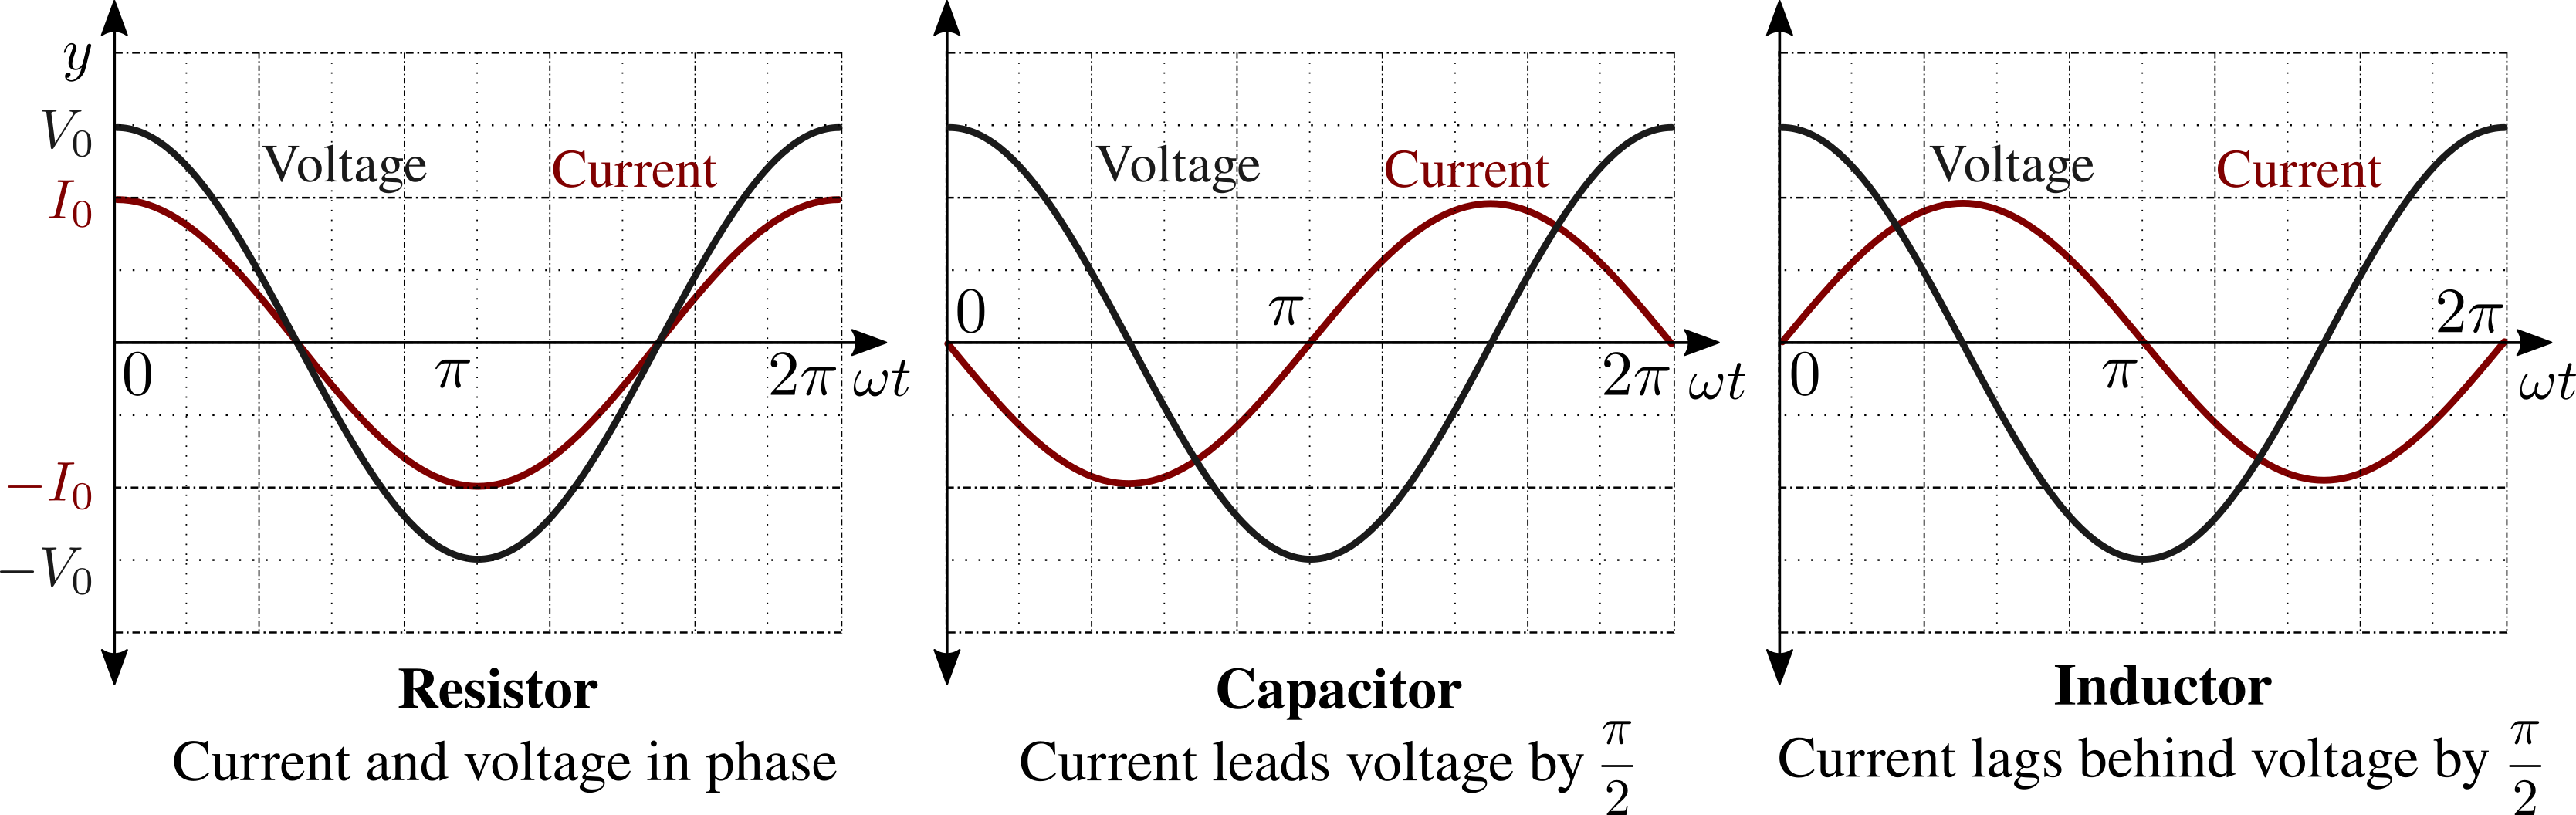
\includegraphics[width=\textwidth]{figs/electronics-circuits/electronics-components-phase-graphs.png}
    \caption{The components described above affect not only the amplitude of the current but also its phase with respect to the applied voltage. For a resistor, the current and voltage are in phase. For a capacitor, the current leads by a phase of $\pi/2$. For an inductor, the current lags by the same phase of $\pi/2$. In order to decide whether the current lags or leads, first ask yourself how much you need to move the current curve so that it is in phase with the voltage. If, for example, you need to move the curve rightward, this means that the current at an \textsl{earlier} time was at the same phase as the voltage at a \textsl{later} time. This implies that the current leads the voltage.  }
    \label{fig:phase-graphs}
\end{figure}



\begin{question}
    \textbf{Question:} Consider a simple time-varying voltage 
    \begin{equation}
        V(t) = V_0 e^{i\omega t},
    \end{equation}
    where $V_0$ is real. Show that the resulting (real) current in the case of each of the above components is given by
    \begin{equation}
        \begin{aligned}
            I_R &= \frac{V_0}{R} \cos(\omega t),\\[10pt]
            I_C &= - \omega C V_0 \sin(\omega t),\\[10pt]
            I_L &= + \frac{V_0}{L} \sin(\omega t).
        \end{aligned}
    \end{equation}

    \textbf{Question:} Use this to show that
    \vspace{-\parskip}
    \begin{enumerate}
    \itemsep0em
        \item In resistors, the current and voltage are in phase,
        \item In capacitors, the current leads the voltage by a phase of $\pi/2$,
        \item In inductors, the current lags behind the the voltage by a phase of $\pi/2$.  
    \end{enumerate}
\end{question}

\begin{imp}
    Often, purely imaginary quantities $z_C$ and $z_L$ are known as ``reactance'', to distinguish themselves from the resistance. There is some merit in this, since these two quantities change both the magnitude of the current, as well as its \textsl{phase}. Resistance, on the other hand, being purely real, only affects the magnitude of the current. However, in our analyses we will just use the general terms impedance for all types of $z$. This is shown graphically in Figure~(\ref{fig:phase-graphs})
\end{imp}



\subsection*{The RC circuit}

We will now try to combine two components -- a resistor and a capacitor -- in a simple circuit. Consider first a capacitor being charged by a DC power source. As the key in switched on, the power source establishes a potential difference across the plates of the capacitor and stores some charge on them. The amount of charge stored is given by the definition of the capacitance in Equation~(\ref{eqn:def-cap}).

If the switch is now disconnected, the capacitor would hold this charge indefinitely. However, if the capacitor is allowed to discharge through a resistor, a current is set up in the circuit which dissipates the energy stored in the capacitor. Using Kirchoff's voltage law to this closed loop, the voltage drop across the resistor ad capacitor should add up to the applied voltage.

\begin{question}
\paragraph{Question:} Using Ohm's Law ($V=IR$) and the definition of capacitance ($Q=CV$), show that this means that:
\begin{equation*}
    R \dv{Q}{t} + \frac{Q}{C} = V_0
\end{equation*}
where $Q(t)$ is the instantaneous charge on the capacitor.

\paragraph{Question:} Solve this (simple) first-order differential equation for the following initial conditions:
\begin{enumerate}
    \item \textbf{Discharging:} The capacitor is initially charged $Q(0) = Q_0$, and is allowed to discharge. (There is no voltage source in the circuit.) \hfill\textbf{Answer:} $Q(t) = Q_0\,\, e^{-t/RC}.$
    
    \item \textbf{Charging:} The capacitor is initially uncharged $Q(0) = 0$, and is allowed to charge from a voltage source $V_0$.
    \hfill\textbf{Answer:} $Q(t) = Q_0\,\, \left(1 - e^{-t/RC}\right).$
\end{enumerate}
\end{question}


An important result from the above analysis is that we can construct a quantity of dimension time, $\tau = RC$, which is the natural time scale of charging or discharging the capacitor through the resistor. This quantity is often called the \textsl{time-constant} of the $RC$ circuit.

\subsection*{The RC circuit as an integrator and a differentiator}

Despite its simplicity, the $RC$ circuit can be used to perform complex tasks. Let us now consider how such a circuit responds to an AC signal of frequency $\omega$. In this case, the input and output voltages of our system are 
\begin{equation}
        V_\text{in}(t) = \widetilde{V}_\text{in} e^{i\omega t} \quad \quad \text{and} \quad \quad V_\text{out}(t) = \widetilde{V}_\text{out} e^{i\omega t}.
\end{equation}

We now have two different time-scales in our problem: one time-scale is the ``natural'' time-scale of the $RC$ circuit ($\tau = RC$), and the other is the time-period associated with the AC signal of frequency $\omega$. 

\subsubsection*{The RC integrator}

Consider what happens when we take the output voltage across the capacitor at \textsl{high} frequency, meaning that we choose a frequency 
\begin{equation}
    \omega \gg \frac{1}{RC}.
\end{equation}

Over this short time-scale, the capacitor barely has time to charge, and therefore the voltage across it is very small. In other words, the input voltage is almost completely dropped over the resistor,
\begin{equation}
    V_\text{in} \approx V_R.
\end{equation}

\begin{question}
    \textbf{Question:} Show the above result in the following way: first show that the current in the circuit is given by
    \begin{equation}
        I = \dfrac{V_\text{in}}{R + \dfrac{1}{i\omega C}}.
        \label{eqn:RC-current}
    \end{equation}

    Next, using the fact that $\omega \gg 1/RC$, show that this just means that 
    \begin{equation}
        I(t) \approx \frac{V_\text{in} (t)}{R},
        \label{eqn:high-freq-current}
    \end{equation}
    which is simply Ohm's law that we saw in Equation~(\ref{eqn:ohms-law}).

    Thus argue that $V_\text{in} \approx V_R$, the potential drop across the resistor.
\end{question}

We will now use this fact to show that in the high-frequency regime the voltage across the capacitor can be written as the \textsl{integral} of the input voltage.

We do this by realising that
\begin{equation}
    Q(t) = C V_C(t) \quad \quad \implies \quad \quad I_C(t) = C \dv{V_C}{t},
\end{equation}

where $Q(t)$ is the charge on the capacitor, $V_C(t)$ is the voltage across the capacitor, and $I_C(t)$ is the  current flowing through the capacitor at the instant $t$.

However, the resistor and capacitor are in series, and therefore the current going through them \textsl{must be the same}! As a result, we can use Equation~(\ref{eqn:high-freq-current}) to show that
\begin{equation}
    V_\text{in} (t) \approx RC \dv{V_C}{t} \quad \quad \implies \quad \quad V_C(t) \approx \frac{1}{RC} \int_0^t V_\text{in}(u)\,\,\dd u.
\end{equation}

Thus, in the high-frequency regime, the voltage across the capacitor is proportional to the \textsl{integral} of the input voltage. Such a configuration can therefore be used to perform integration!

\subsubsection*{The RC differentiator}

Let us now consider the output across the resistor in the \textsl{low-}frequency regime, i.e. when
\begin{equation}
    \omega \ll \frac{1}{RC}.
\end{equation}
\begin{question}
    \textbf{Question:} Using Equation~(\ref{eqn:RC-current}), show that
    \begin{equation}
        V_\text{in} \approx \frac{1}{i \omega C} = V_C, \quad \text{when} \quad \omega \ll \frac{1}{RC}.
    \end{equation}
\end{question}

Since the configuration is still a series configuration, the current across the capacitor is the same as the total current in the circuit. As a result, we can say -- just as before -- that 
\begin{equation}
    I= \dv{Q}{t} = C \dv{V_C}{t}.
\end{equation}
\begin{question}
    \textbf{Question:} Using the above relations, show that you can write 
    \begin{equation}
        V_R = IR \quad \quad \implies V_R(t) \approx RC \dv{V_\text{in}}{t}, \quad \text{when} \quad \omega \ll \frac{1}{RC}.
    \end{equation}
\end{question}

In other words, in the low-frequency regime, the voltage across the resistor is approximately the \textsl{derivative} of the input voltage.

An $RC$ circuit can thus be used to perform the mathematical operations of integration and differentiation. However, these values are -- as explained above -- only approximate. More accurate integration and differentiation can be achieved combining the above circuits with a device called an \textsl{operational amplifier} or op-amp. However, this is far beyond the scope of this experiment.

\begin{imp}
\begin{itemize}
    \itemsep0em
    \item In the high-frequency regime, $V_C$ is the integral of the input voltage.
    \item In the low-frequency regime,  $V_R$ is the derivative of the input voltage.
\end{itemize}
\end{imp}
The two configurations described above are shown in Figure~(\ref{fig:RC-configs}).

\begin{figure}
    \centering
    \begin{subfigure}[b]{0.45\textwidth}
        \centering
        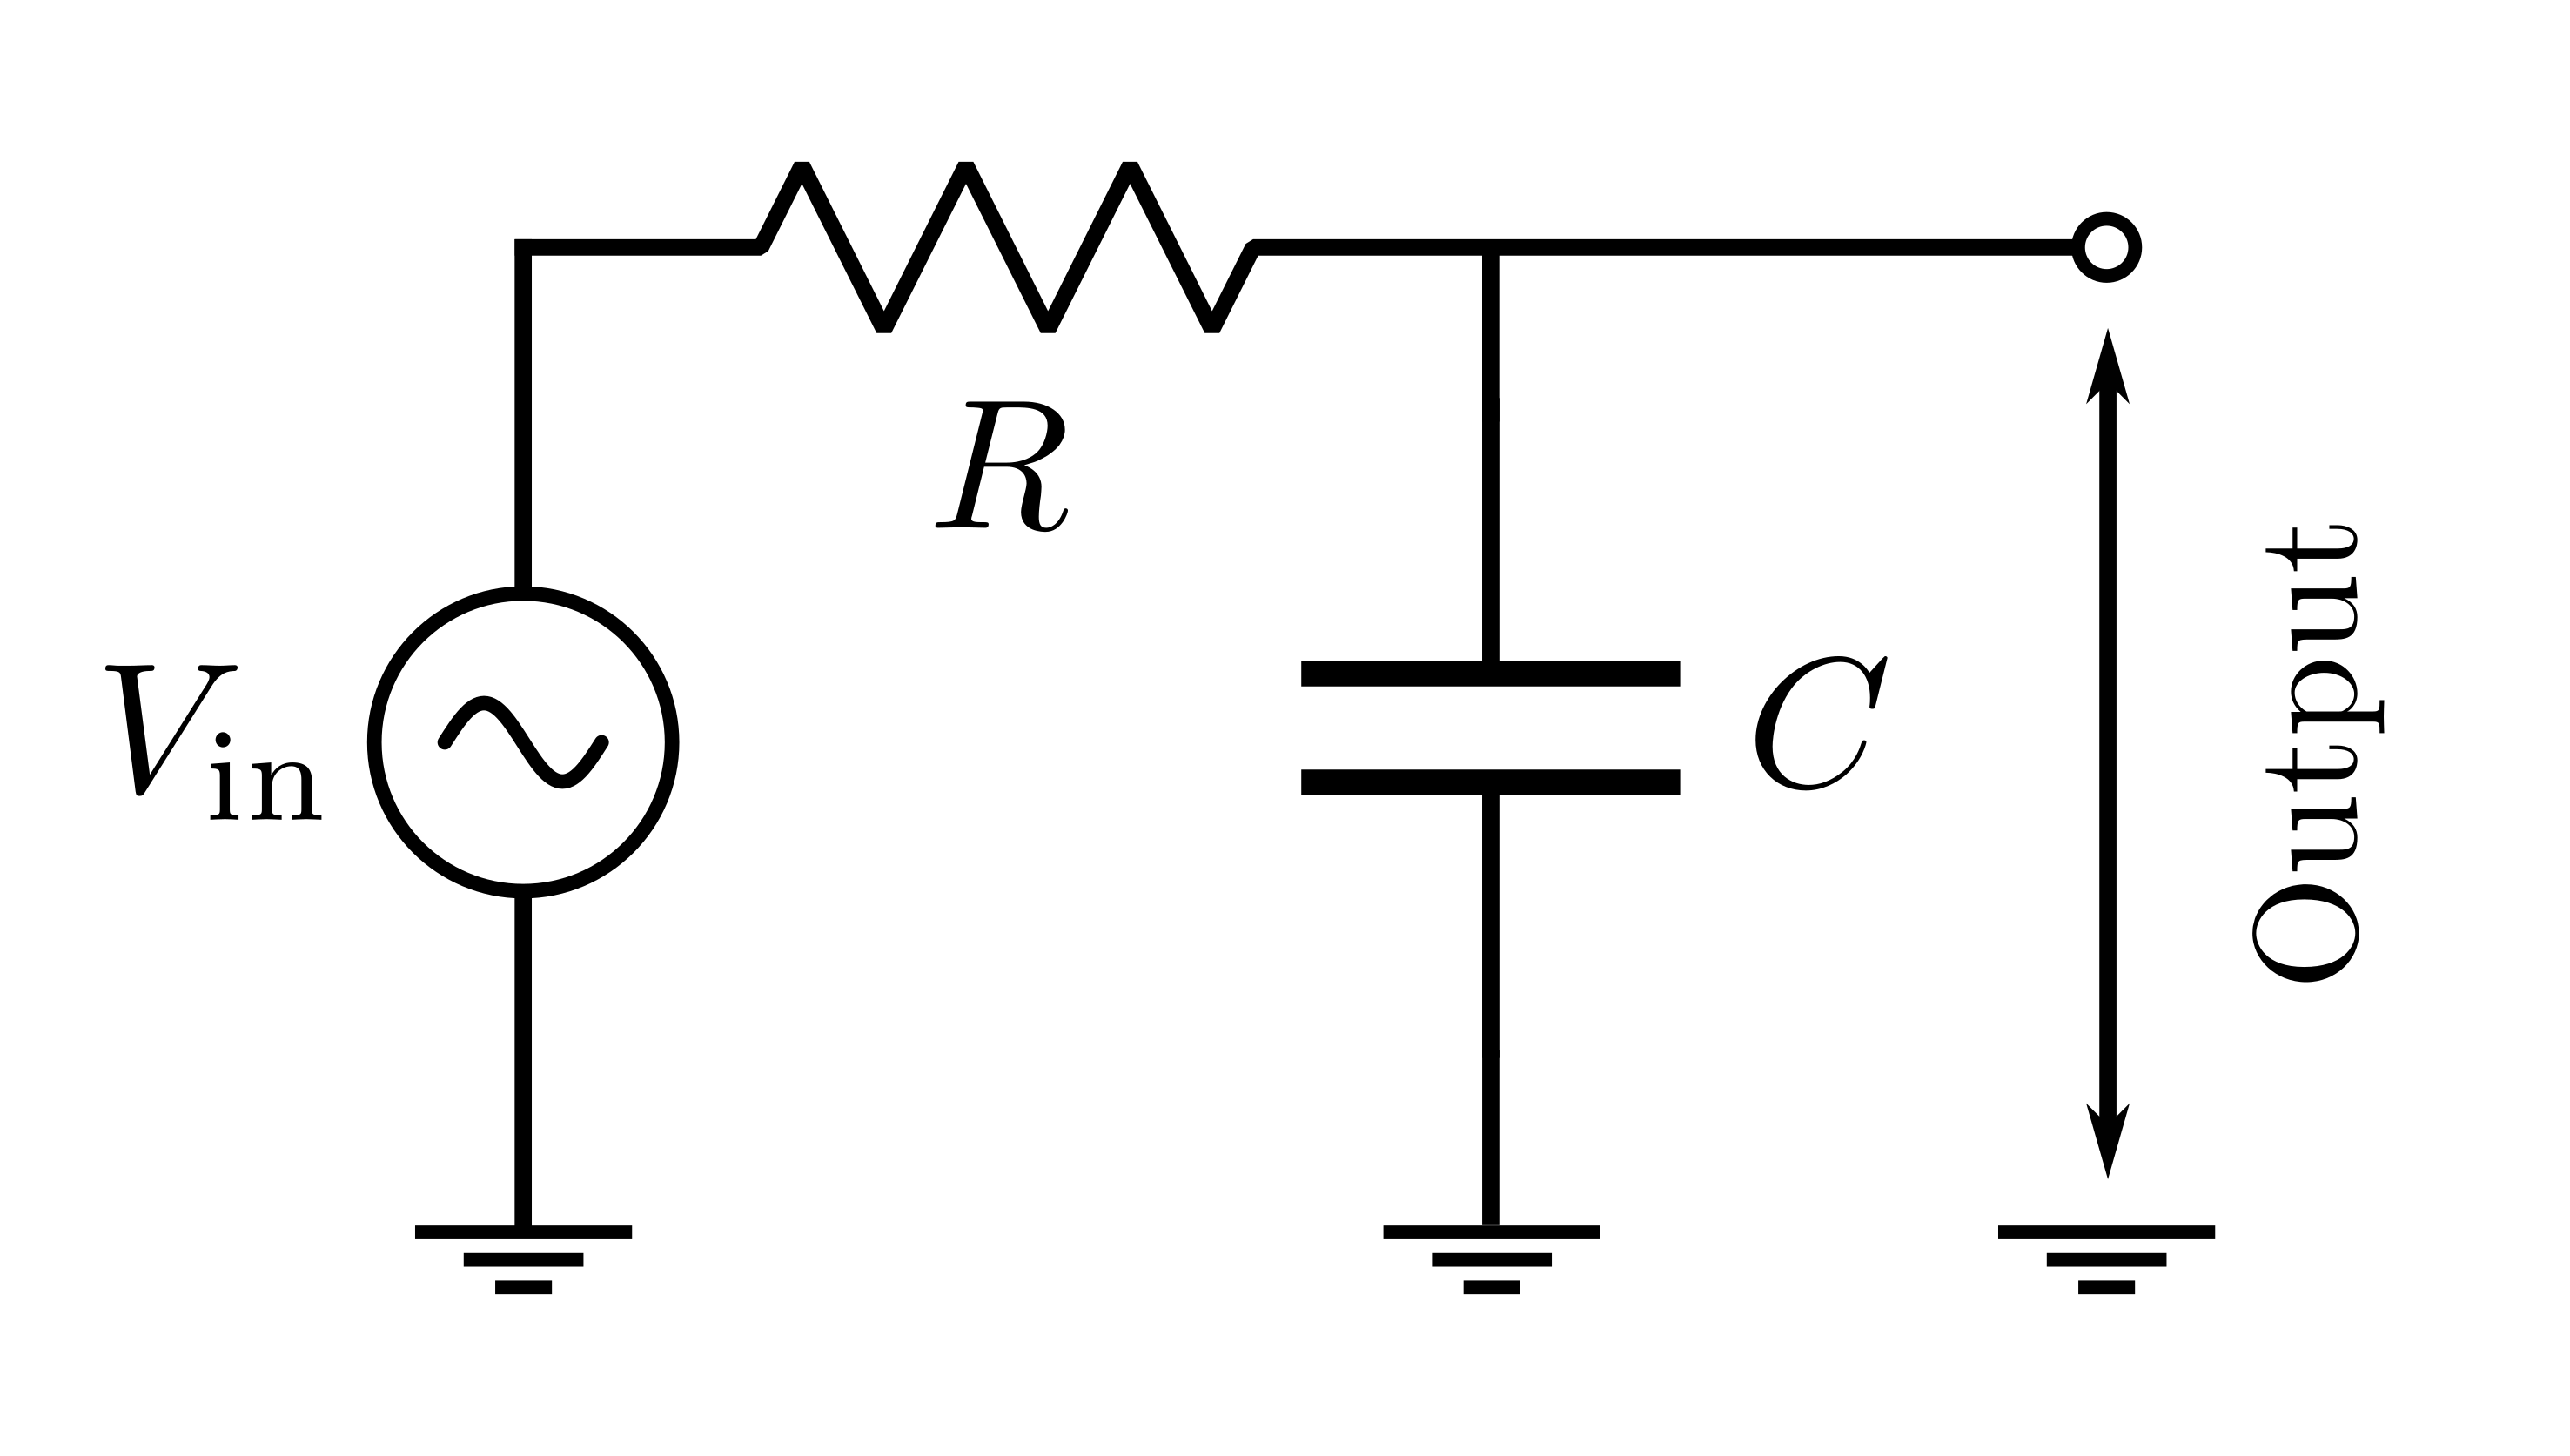
\includegraphics[width=\textwidth]{figs/electronics-circuits/RCLP.png}
        \caption{The RC integrator and low-pass filter}
        \label{fig:rc-lp}
    \end{subfigure}\hfill
    \begin{subfigure}[b]{0.45\textwidth}
        \centering
        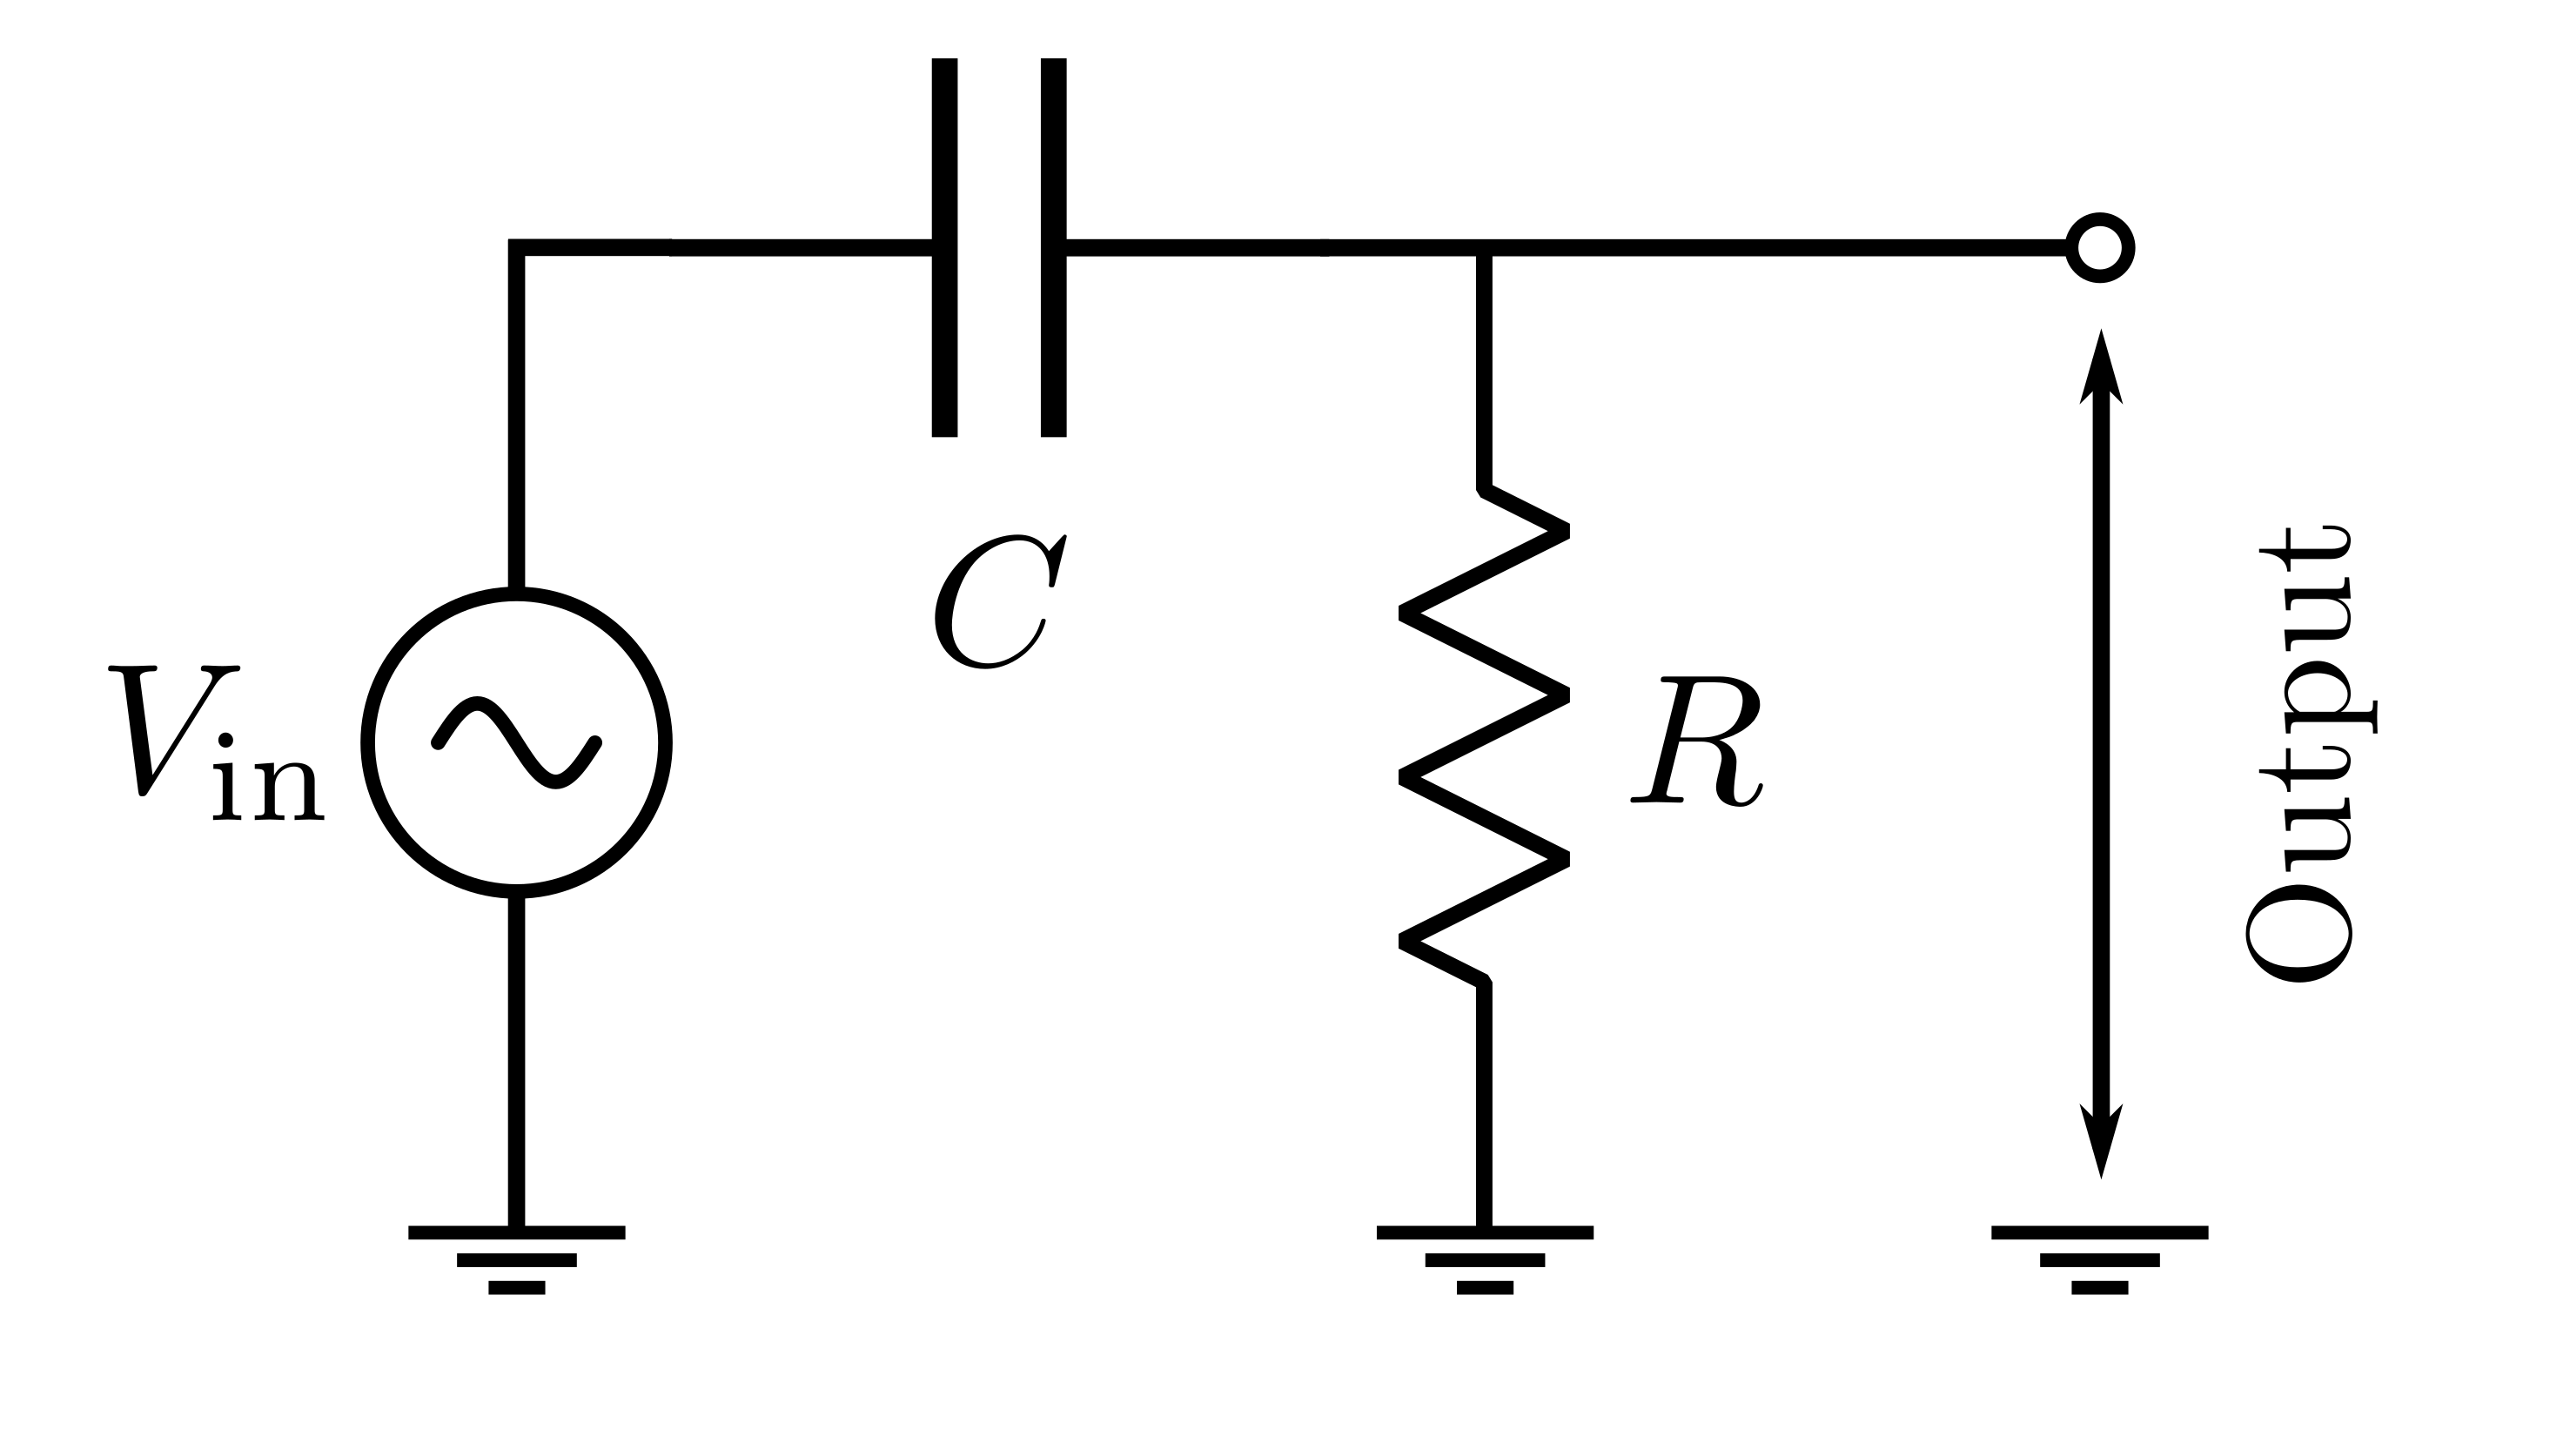
\includegraphics[width=\textwidth]{figs/electronics-circuits/RCHP.png}
        \caption{The RC differentiator and high-pass filter}
        \label{fig:rc-hp}
    \end{subfigure}
    \caption{Different possible configurations for an $RC$ circuit. In (a) we see the configuration that works both as a integrator and a low-pass filter, while in (b) we see the configuration that works both as a differentiator and a high-pass filter.}
    \label{fig:RC-configs}
\end{figure}

\subsection*{The RC circuit as a filter}

In our analysis so far, we have considered the time-series behaviour of our system: a time-varying signal can be either integrated or differentiated based on the $RC$ configuration. However, the above analysis has another interesting consequence. As we have seen above, in the case of the ``integrator'' configuration $V_R \approx V_\text{in}$. Thus the output voltage across the capacitor is essentially zero at high-frequencies. In other words, such a configuration \textsl{blocks} high frequencies when compared to low frequencies. When this occurs, we say that the $RC$ circuit is working as a \textsl{low-pass} filter, as it allows low frequencies to pass undisturbed, and attenuates high frequencies.

Similarly, in the ``differentiator'' configuration, we have seen that $V_C \approx V_\text{in}$, and therefore the output across the resistor is essentially zero at \textsl{low} frequencies. Therefore, in this particular configuration, high frequencies are allowed to pass essentially undisturbed, and low frequencies are attenuated.

Thus, given an $RC$ circuit we can construct a \textsl{cutoff} frequency $\omega_c = 1/RC$ such that for high-frequencies ($\omega \gg \omega_c$) one configuration -- Figure~(\ref{fig:rc-lp}) -- attenuates these frequencies, and the other -- Figure~(\ref{fig:rc-hp}) -- allows them to pass without modification.

\subsubsection*{Gain, decibels, and Bode plots}

In order to study the response of such filters, we define the concept of a ``gain'' of an electrical circuit. The gain of a circuit is just the ratio of the output to the input voltage. A gain of greater than one means the signal was amplified, while a gain of less than one means it was attenuated. It turns out that a log scale is much more convenient for talking about gains, and so by convention we define a unit called a ``bel'', which is an increase in power by 10 times,
\begin{equation}
    \text{gain in B} = \log_{10}\left( \frac{P_\text{out}}{P_\text{in}} \right).
\end{equation}
The bel is inconveniently large, and for historical reasons\footnote{The bel can be traced back to the old phone and telegraph system. Indeed, the unit was itself named after Alexander Graham Bell, the inventor of the telephone.} it was replaced by a smaller unit, the \textsl{deci}bel: one-tenth of a bel. The gain in units of decibel is 10 times the gain in units of bel,
\begin{equation}
    \text{gain in dB} = 10\,\, \text{ gain in B} = 10 \,\,\log_{10}\left( \frac{P_\text{out}}{P_\text{in}} \right).
\end{equation}
Now, as we have seen, we will be measuring voltages rather than power. For a resistive circuit, for example, we know that $P =V^2/R$, and so we can thus rewrite the earlier equation in terms of the ratio of voltages rather than the ratio of powers, since
\begin{equation}
    \text{gain in dB} = 10 \,\,\log_{10} \left( \frac{V^2_\text{out}}{V^2_\text{in}} \right) = 20 \,\log_{10} \left( \frac{V_\text{out}}{V_\text{in}} \right).
\end{equation}

Lastly, all the plots dealing with the gain are often ``Bode'' plots. In such plots, the $y-$axis is the gain, and the $x-$axis is the frequency in a log scale. This results in a log-log plot, since both the axes are logarithmic variables. We will not go into the reasons for using such plots here (although they are very interesting!) but will instead restrict ourselves to using them.


\subsubsection*{The low-pass and high-pass filters}

Let us now compute the ratio of the output voltage to the input voltage for a low-pass filter. In this configuration, the output voltage is the voltage across the capacitor, and so 
\begin{equation}
    \text{gain} = \frac{V_\text{out}}{V_\text{in}} = \frac{V_C}{V_\text{in}}.
\end{equation}

\begin{question}
    \textbf{Question:} Using the fact that $V_C = I z_C$, and the expression for the current in Equation~(\ref{eqn:RC-current}), show that 
    \begin{equation}
        \frac{V_C}{V_\text{in}} = \frac{1}{1 + i \omega R C}.
    \end{equation}

    \textbf{Question:} The actual gain is the real part of this. Using the fact that if $x$ is a real, then
    \begin{equation}
        \Re \left( \frac{1}{1 + i x }\right) = \frac{1}{\sqrt{1 + x^2}},
    \end{equation}
    % show that
    \begin{equation}
        \text{gain} = \dfrac{1}{\sqrt{1 + \omega^2 R^2 C^2}} = \frac{1}{\sqrt{1 + \left(\omega/\omega_c\right)^2}}.
    \end{equation}
    
\end{question}


Similarly, let us compute the same quantity for the high-pass filter. In this case, the output voltage is taken across the resistor, and therefore
\begin{equation}
    \text{gain} = \frac{V_\text{out}}{V_\text{in}} = \frac{V_R}{V_\text{in}}.
\end{equation}

\begin{question}
    \textbf{Question:} Using the same technique as in the previous question, show that 
    \begin{equation}
        \text{gain} = \dfrac{\omega R C}{\sqrt{1 + \omega^2 R^2 C^2}} = \frac{\left(\omega/\omega_c\right)}{\sqrt{1 + \left(\omega/\omega_c\right)^2}}.
    \end{equation}
\end{question}

The above equations for the gains of the low- and high-pass filters can be plotted. The results are shown in Figure~(\ref{fig:RC-bode}).

\begin{figure}[!htb]
    \centering
    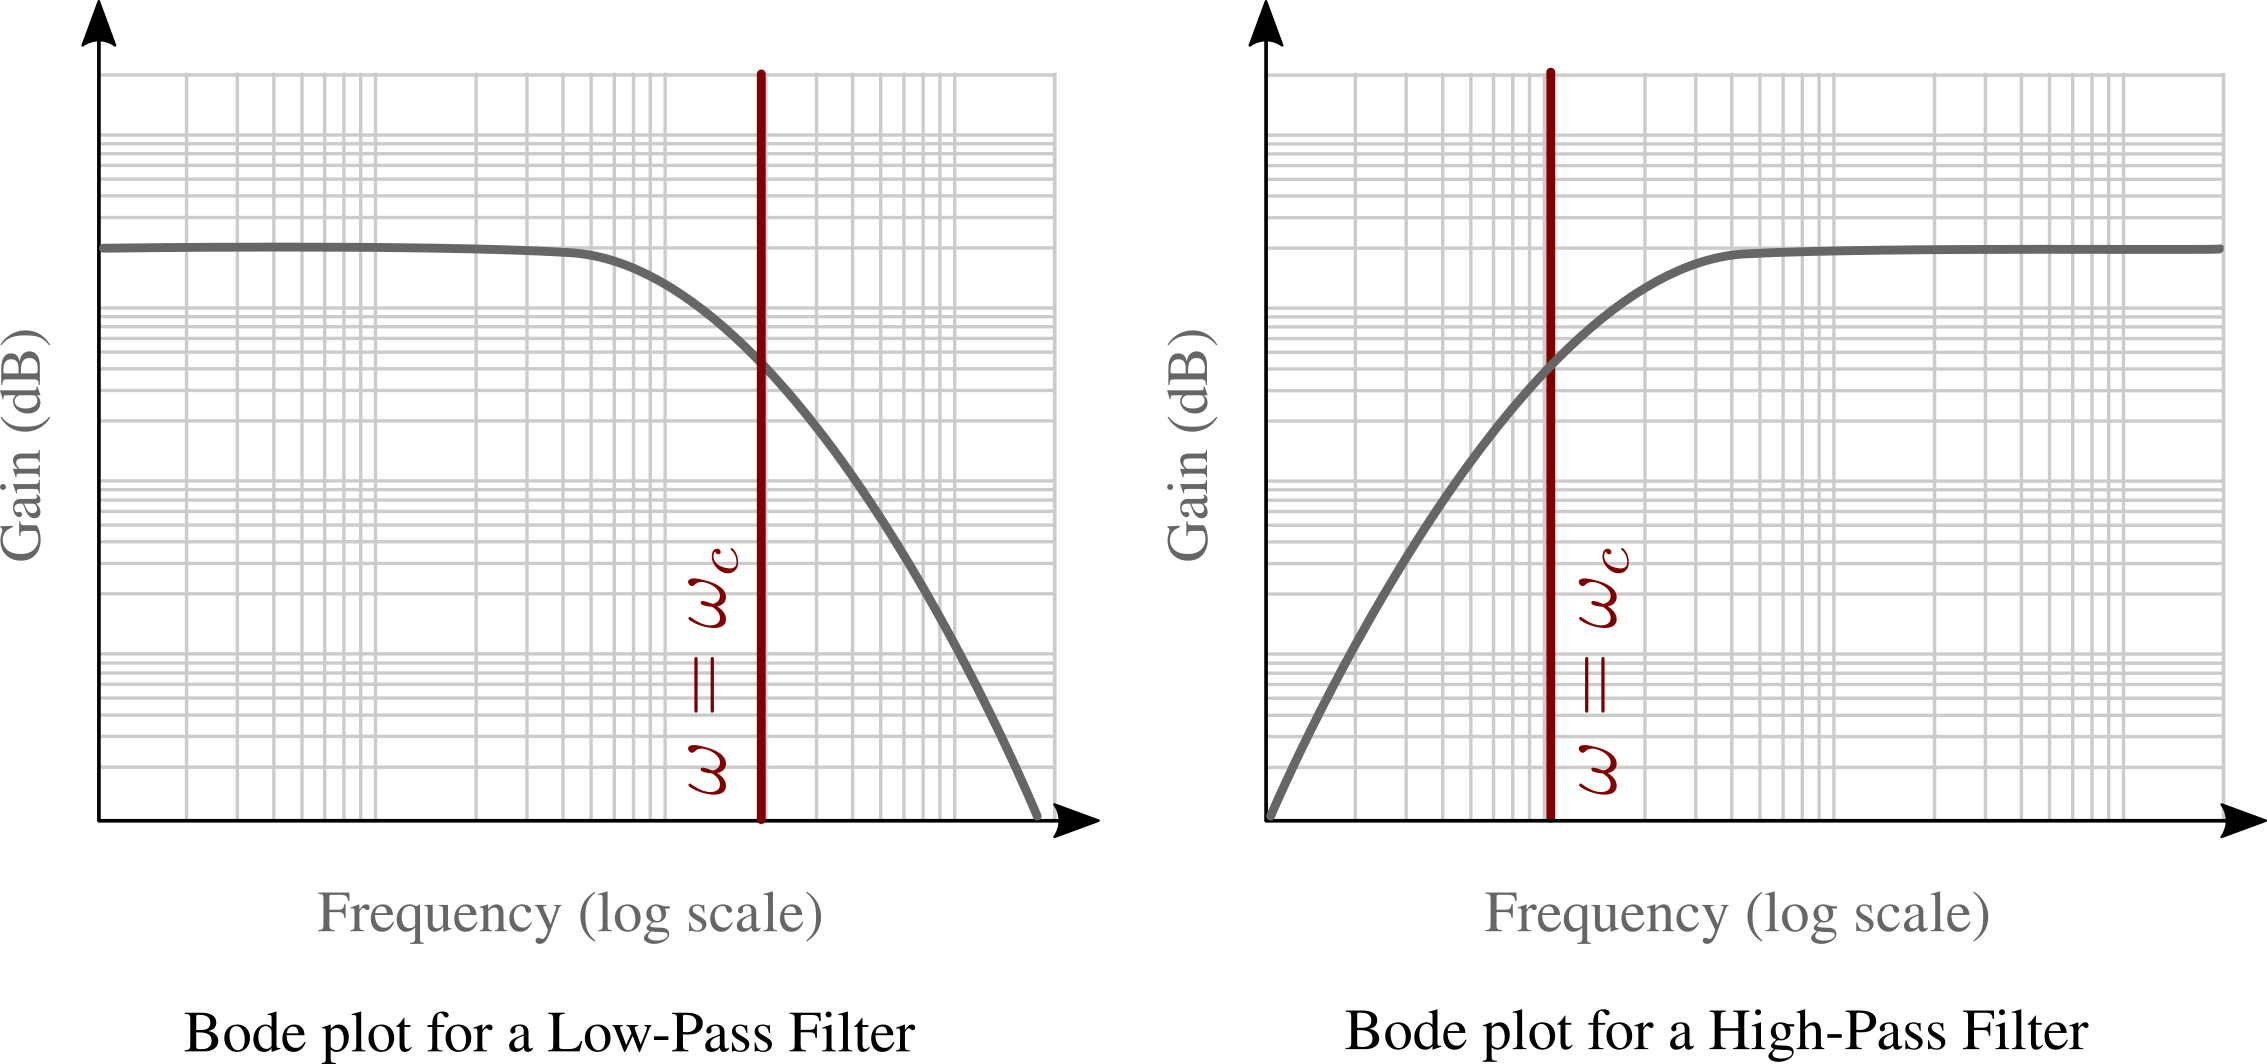
\includegraphics[width=0.9\textwidth]{figs/electronics-circuits/RC-gain.png}
    \caption{Bode plots for the low- and high-pass filters. In both cases, $\omega = \omega_c$ marks a ``knee'' in the graph. In the case of the low-pass filter, the gain (in dB) is initially constant and starts to decrease sharply as $\omega$ becomes greater than $\omega_c$. The converse is true for the high-pass filter: the gain increases sharply reaches a plateau when $\omega$ is greater than $\omega_c$.}
    \label{fig:RC-bode}
\end{figure}

\begin{imp}
    We have discussed different applications of the two circuits shown in Figure~(\ref{fig:RC-configs}), and it is easy to get confused about which configuration can be used for which. A summary at this point would be useful:

    \centering

    \begin{tabular}{@{}cccc@{}}
    \toprule
    \textbf{}                                                            \textbf{Circuit} & \textbf{Output}   & \textbf{Time-domain}  & \textbf{Frequency-domain} \\ \midrule
    \begin{tabular}[c]{@{}c@{}}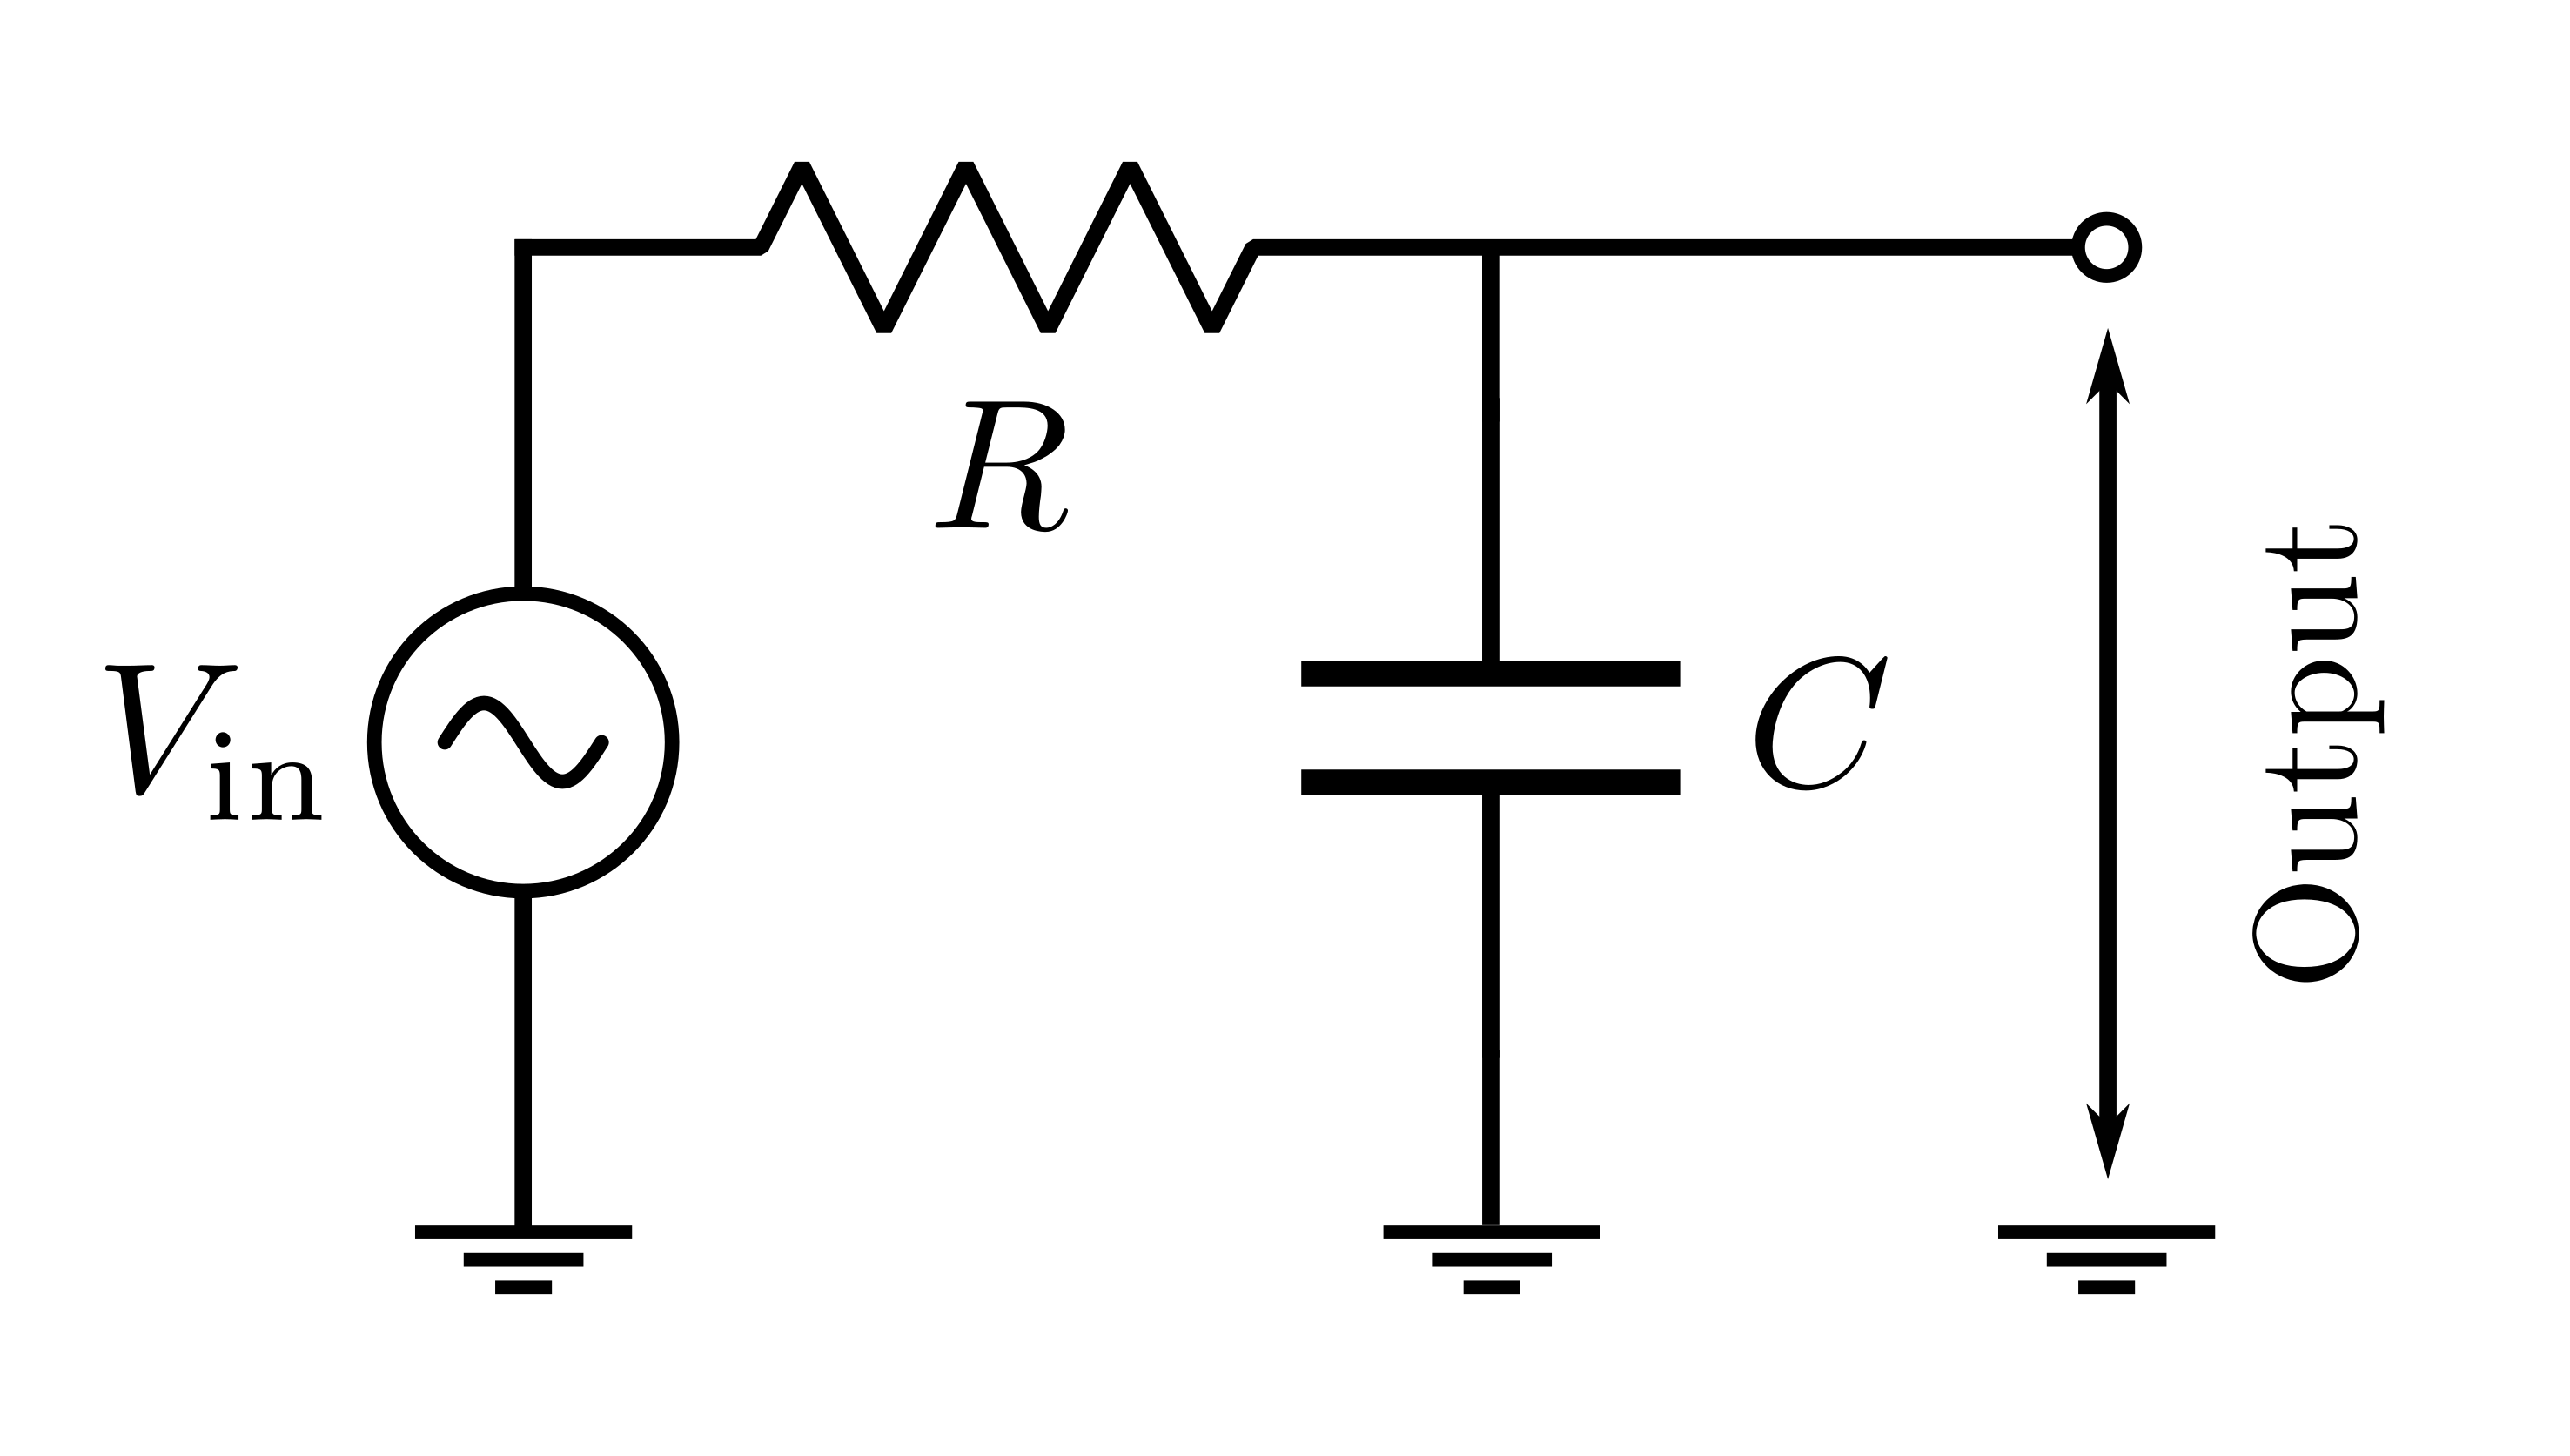
\includegraphics[width=0.23\textwidth]{figs/electronics-circuits/RCLP.png}\end{tabular} &
    \begin{tabular}[c]{@{}c@{}} Across capacitor\\ (see Figure~(\ref{fig:rc-lp}))\end{tabular} & \begin{tabular}[c]{@{}c@{}}Integrator\\ when $\omega \ll \omega_c$\end{tabular}     & Low-pass filter           \\
    \begin{tabular}[c]{@{}c@{}}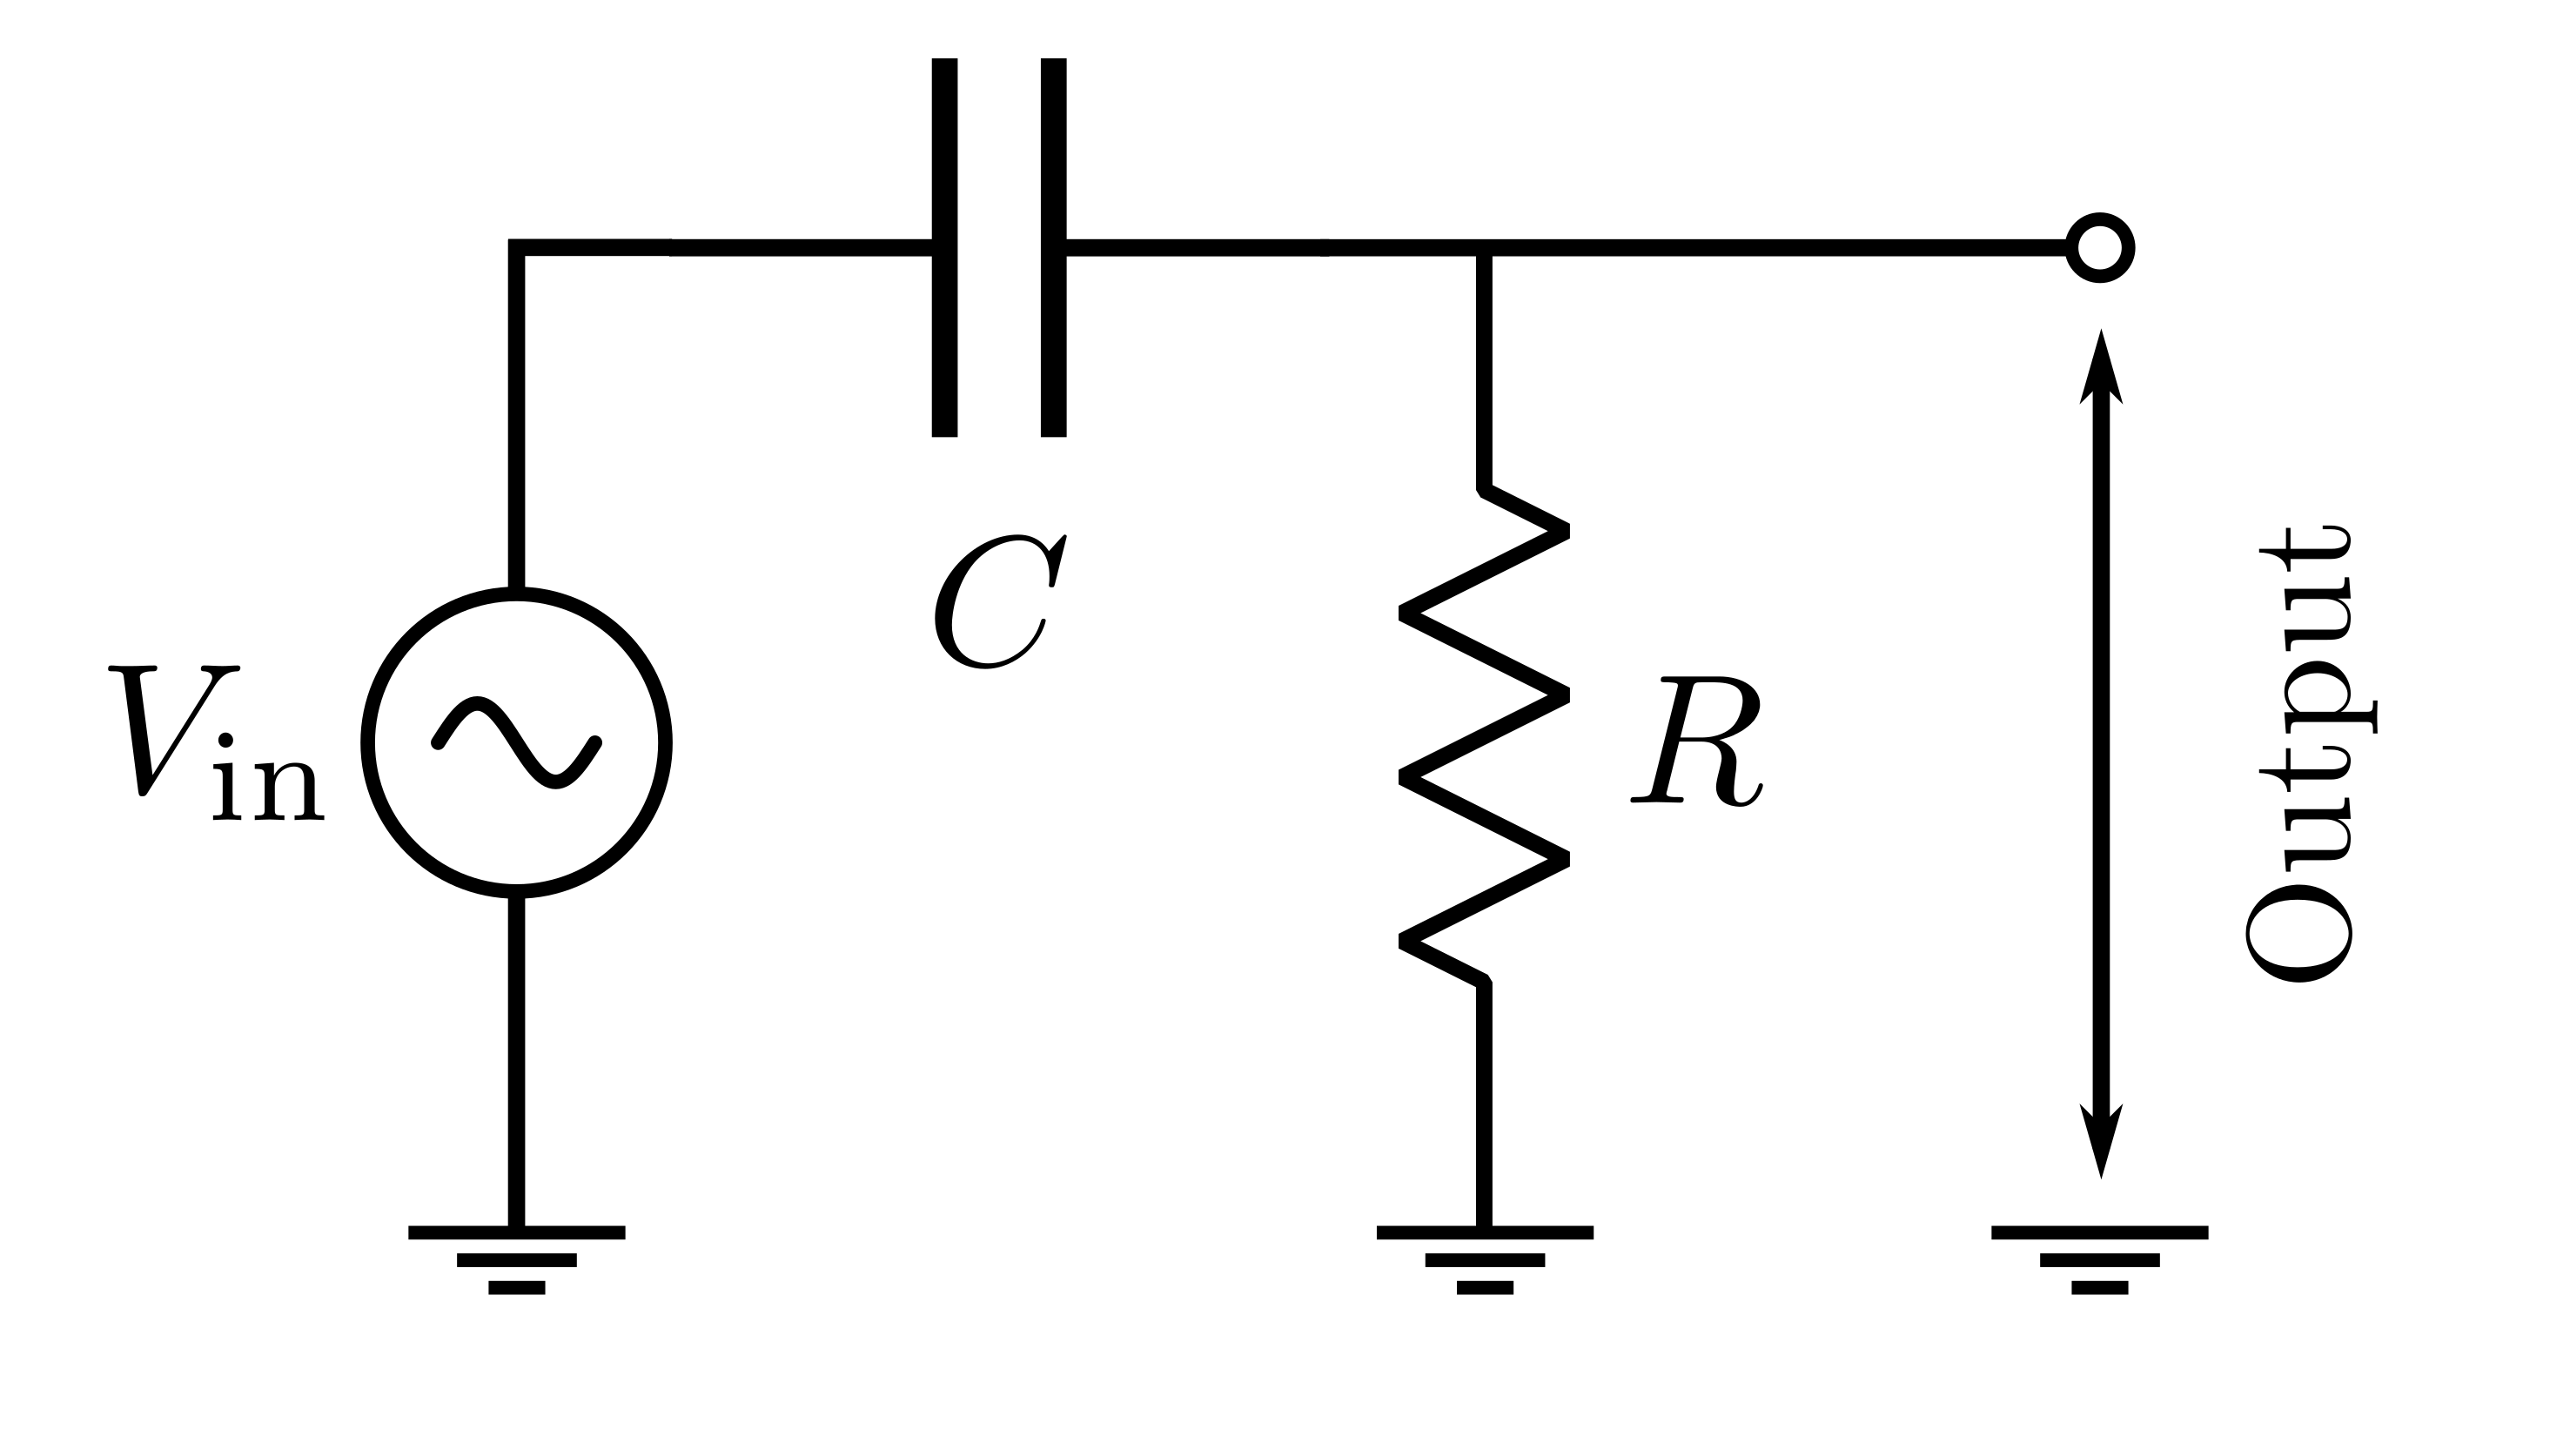
\includegraphics[width=0.23\textwidth]{figs/electronics-circuits/RCHP.png}\end{tabular} & \begin{tabular}[c]{@{}c@{}} Across resistor\\ (see Figure~(\ref{fig:rc-hp})\end{tabular}  & \begin{tabular}[c]{@{}c@{}}Differentiator\\ when $\omega \gg \omega_c$\end{tabular} & High-pass filter          \\ \bottomrule
    \end{tabular}
    
    
\end{imp}


\subsection*{The LCR circuit}

\begin{figure}[!htb]
    \centering
    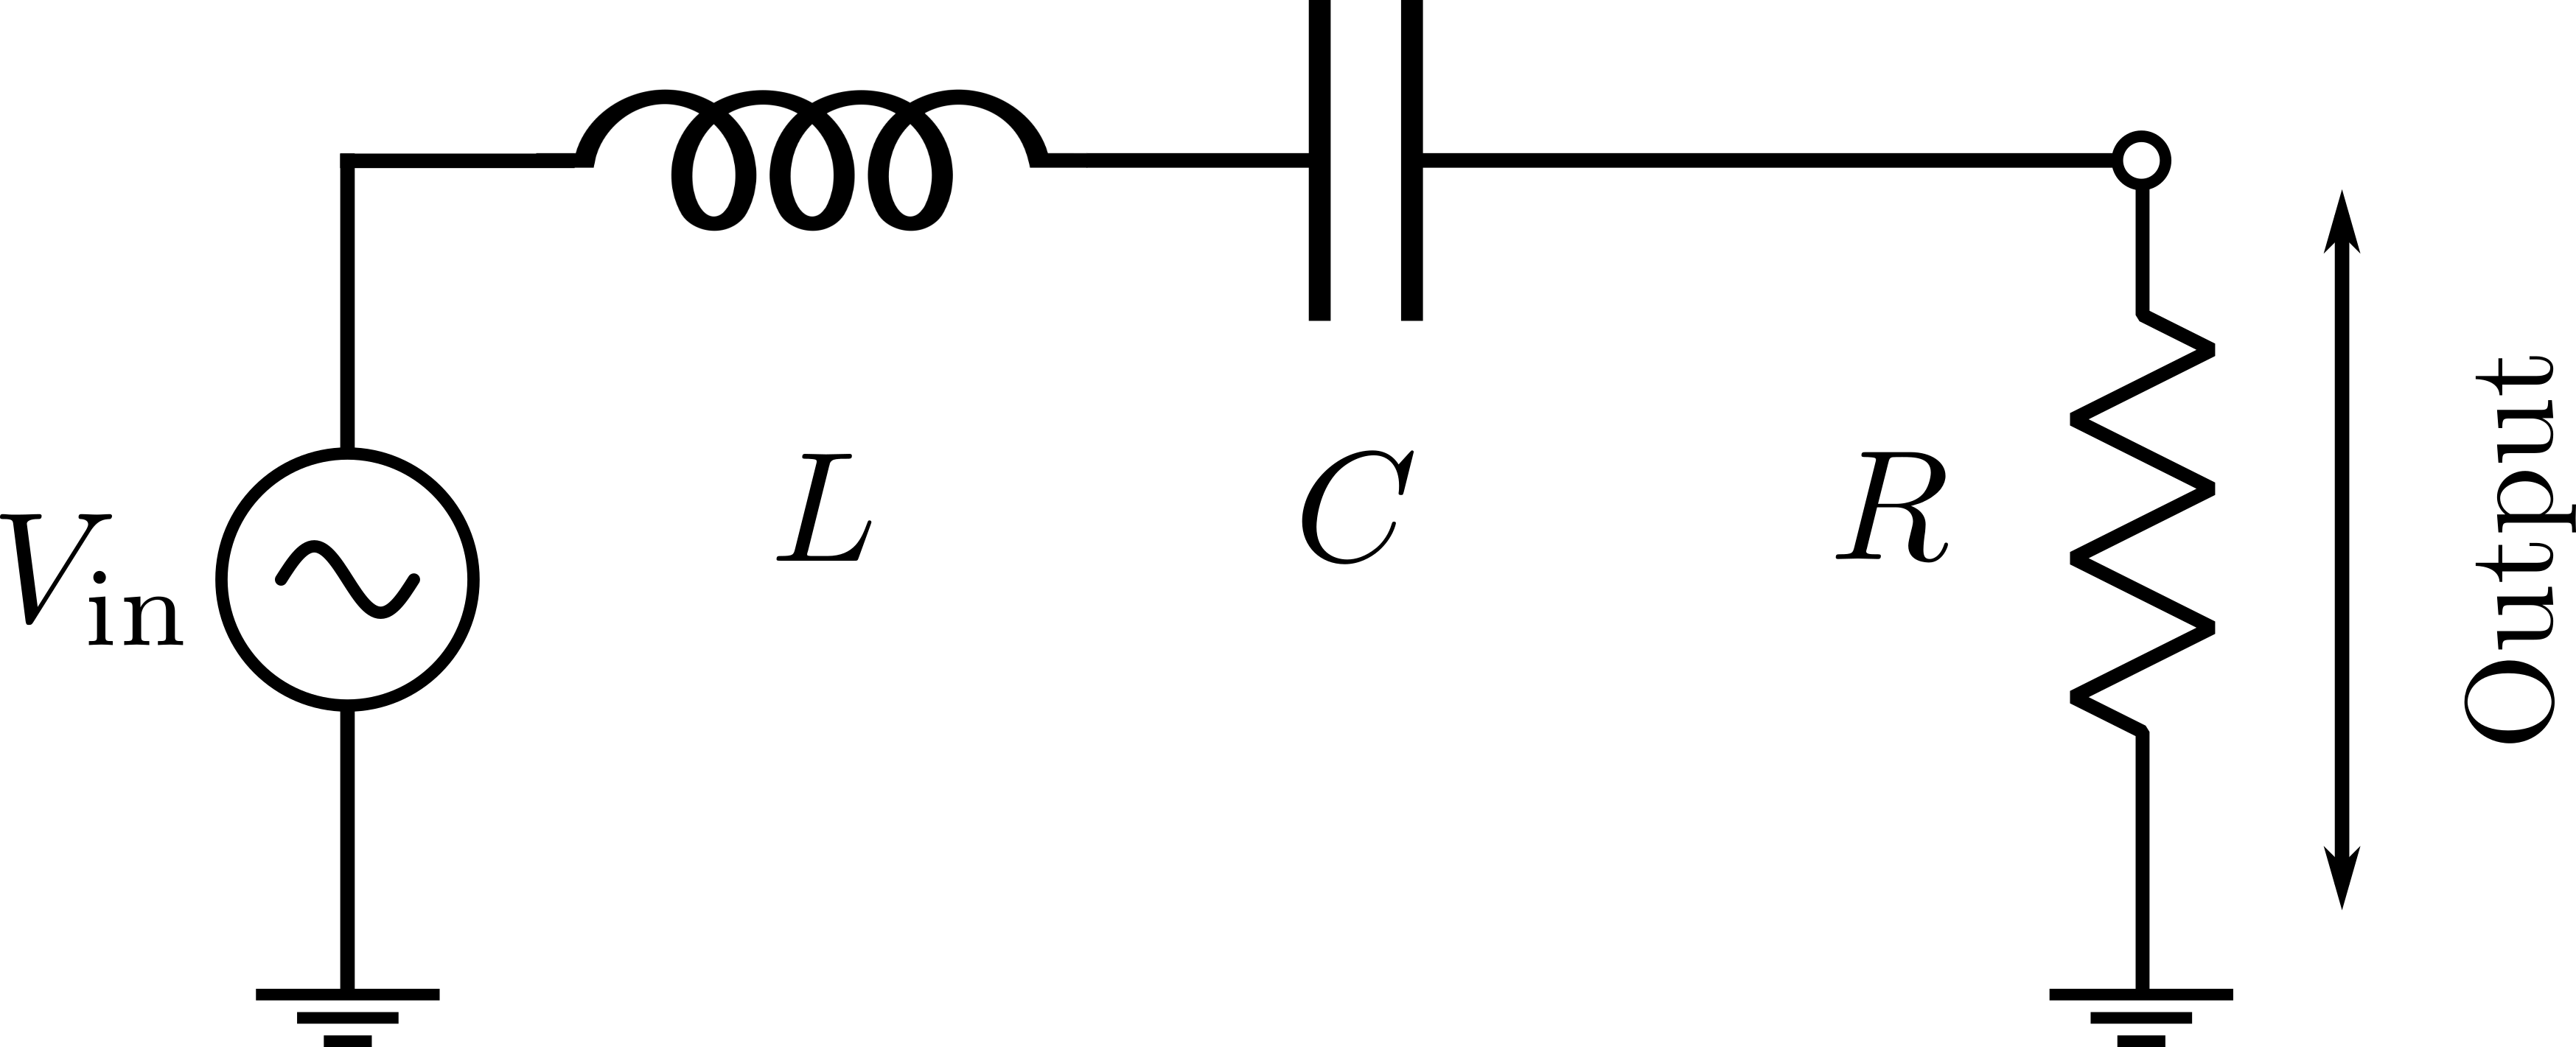
\includegraphics[width=0.65\textwidth]{figs/electronics-circuits/LCRSeries.png}
    \caption{A series $LCR$ circuit. The inductor, capacitor, and resistor are attached to an AC power supply, and the output voltage is taken across the resistor. }
    \label{fig:lcr-series}
\end{figure}

We are now ready to study a more complicated circuit: consider a series combination of an inductor, capacitor, and resistor, as shown in Figure~(\ref{fig:lcr-series}). As with the $RC$ circuit, we first study the natural response of this system: how does it behave in the absence of any external driving force. Using Kirchoff's law, you should be able to show that since the potential drop across the various components in the closed circuit loop is zero, we have
\begin{equation}
    L \dv{I}{t} + R I + \frac{Q}{C} = 0.
\end{equation}

In itself, this equation may not look too familiar to you, but if you divide it by $L$ and take a derivative of the left-hand side with respect to time, you should be able to see that the equation becomes very familiar:
\begin{equation}
    \dv[2]{I}{t} + \gamma \dv{I}{t} + \omega_0^2 I = 0.
\end{equation}

This is just the differential equation for a damped harmonic oscillator with natural frequency $\omega_0$ and a damping coefficient of $\gamma$.

\begin{question}
    \textbf{Question:} Show that 
    \begin{equation}
        \omega_0 = \frac{1}{\sqrt{LC}}, \quad \quad \text{and} \quad \quad \gamma = \frac{R}{L}.
    \end{equation}
\end{question}

The analogy with the damped harmonic oscillator means that the form of this differential equation already allows us to draw some important conclusions:
\begin{itemize}
    \item If the resistance is not too high (i.e. if $\gamma < 2 \omega_0$ or $R < 2 \sqrt{L/C}$) the current in the circuit executes damped harmonic oscillations of the form
    \begin{equation}
        I(t) = I_0 e^{-\gamma t/2} \cos(\omega_1 t - \varphi),
    \end{equation}

    where $I_0$ and $\varphi$ are constants set by the initial conditions, and $\omega_1 = \sqrt{\omega_0^2 - \gamma^2/4}$.

    \item For values of resistance greater than $2 \sqrt{L/C}$, the system does not naturally exhibit oscillations, as is considered to be \textsl{overdamped}.

    \item The resistance plays the role of the dissipative term, allowing the system to lose energy. The inductance plays the role of the mass, and the capacitance the role of the spring-constant.
\end{itemize}

Introducing an AC signal to such a system is equivalent to driving a damped harmonic oscillator. Therefore, we should expect to see phenomena like resonance that you should already be familiar with from your study of mechanical systems.

\subsection*{Resonance in an $LCR$ oscillator}
Consider an $LCR$ circuit of some natural frequency $\omega_0$ being driven by an external AC frequency of $\omega$. As before, we consider that the voltage and current are both oscillating at the same frequency $\omega$. We can easily compute the net impedance of our series $LCR$ circuit as
\begin{equation}
    \begin{aligned}
        z &= z_L + z_C + z_R,\\
          &= i\omega L + \frac{1}{i\omega C} + R,\\ 
          &= R + i \left( \omega L - \frac{1}{\omega C} \right).
    \end{aligned}
\end{equation}

The current in this circuit is thus simply given by 
\begin{equation}
    I = \frac{V_\text{in}}{z} = \frac{V_\text{in}}{R + i  \left( \omega L - \dfrac{1}{\omega C} \right) }.
\end{equation}

\begin{question}
    \textbf{Question:} Show that the oscillator will draw the highest current from the power supply when 
    \begin{equation}
        \omega L = \frac{1}{\omega C}, \quad \iff \quad \omega = \frac{1}{\sqrt{LC}} = \omega_0. 
    \end{equation}

    This is called \textsl{resonance}.

    \textbf{Question:} Show that for such a ``series'' $LCR$ circuit (i) the net impedance is $0$ at both $\omega \to 0$ and $\omega\to\infty$, and (ii) at resonance, the net impedance is $z=R$.
\end{question}

Thus, when $\omega = \omega_0$, the impedance of the system is minimum and consequently, the system draws the greatest power from the power supply. As one moves away from $\omega=\omega_0$ on either side, the current drawn by the system reduces. We thus get a ``band'' over which the current is large, and beyond which the current falls rapidly. 

% The way that this happens depends on the \textsl{quality factor} of our oscillator, defined by
% \begin{equation}
%     \mathcal{Q} = \frac{\omega_0}{\gamma} = \frac{1}{R}\sqrt{\frac{L}{C}}.
% \end{equation}

% Clearly, when $R\to0$, the quality factor of 

The configuration shown in Figure~(\ref{fig:lcr-series}) is of course only one of many possible ways in which inductors, capacitors, and resistors can be combined. Another possible combination is to keep the components in \textsl{parallel}. One such configuration, known as a \textsl{tank} circuit, is shown in Figure~(\ref{fig:lcr-parallel}). 

\begin{figure}[!htb]
    \centering
    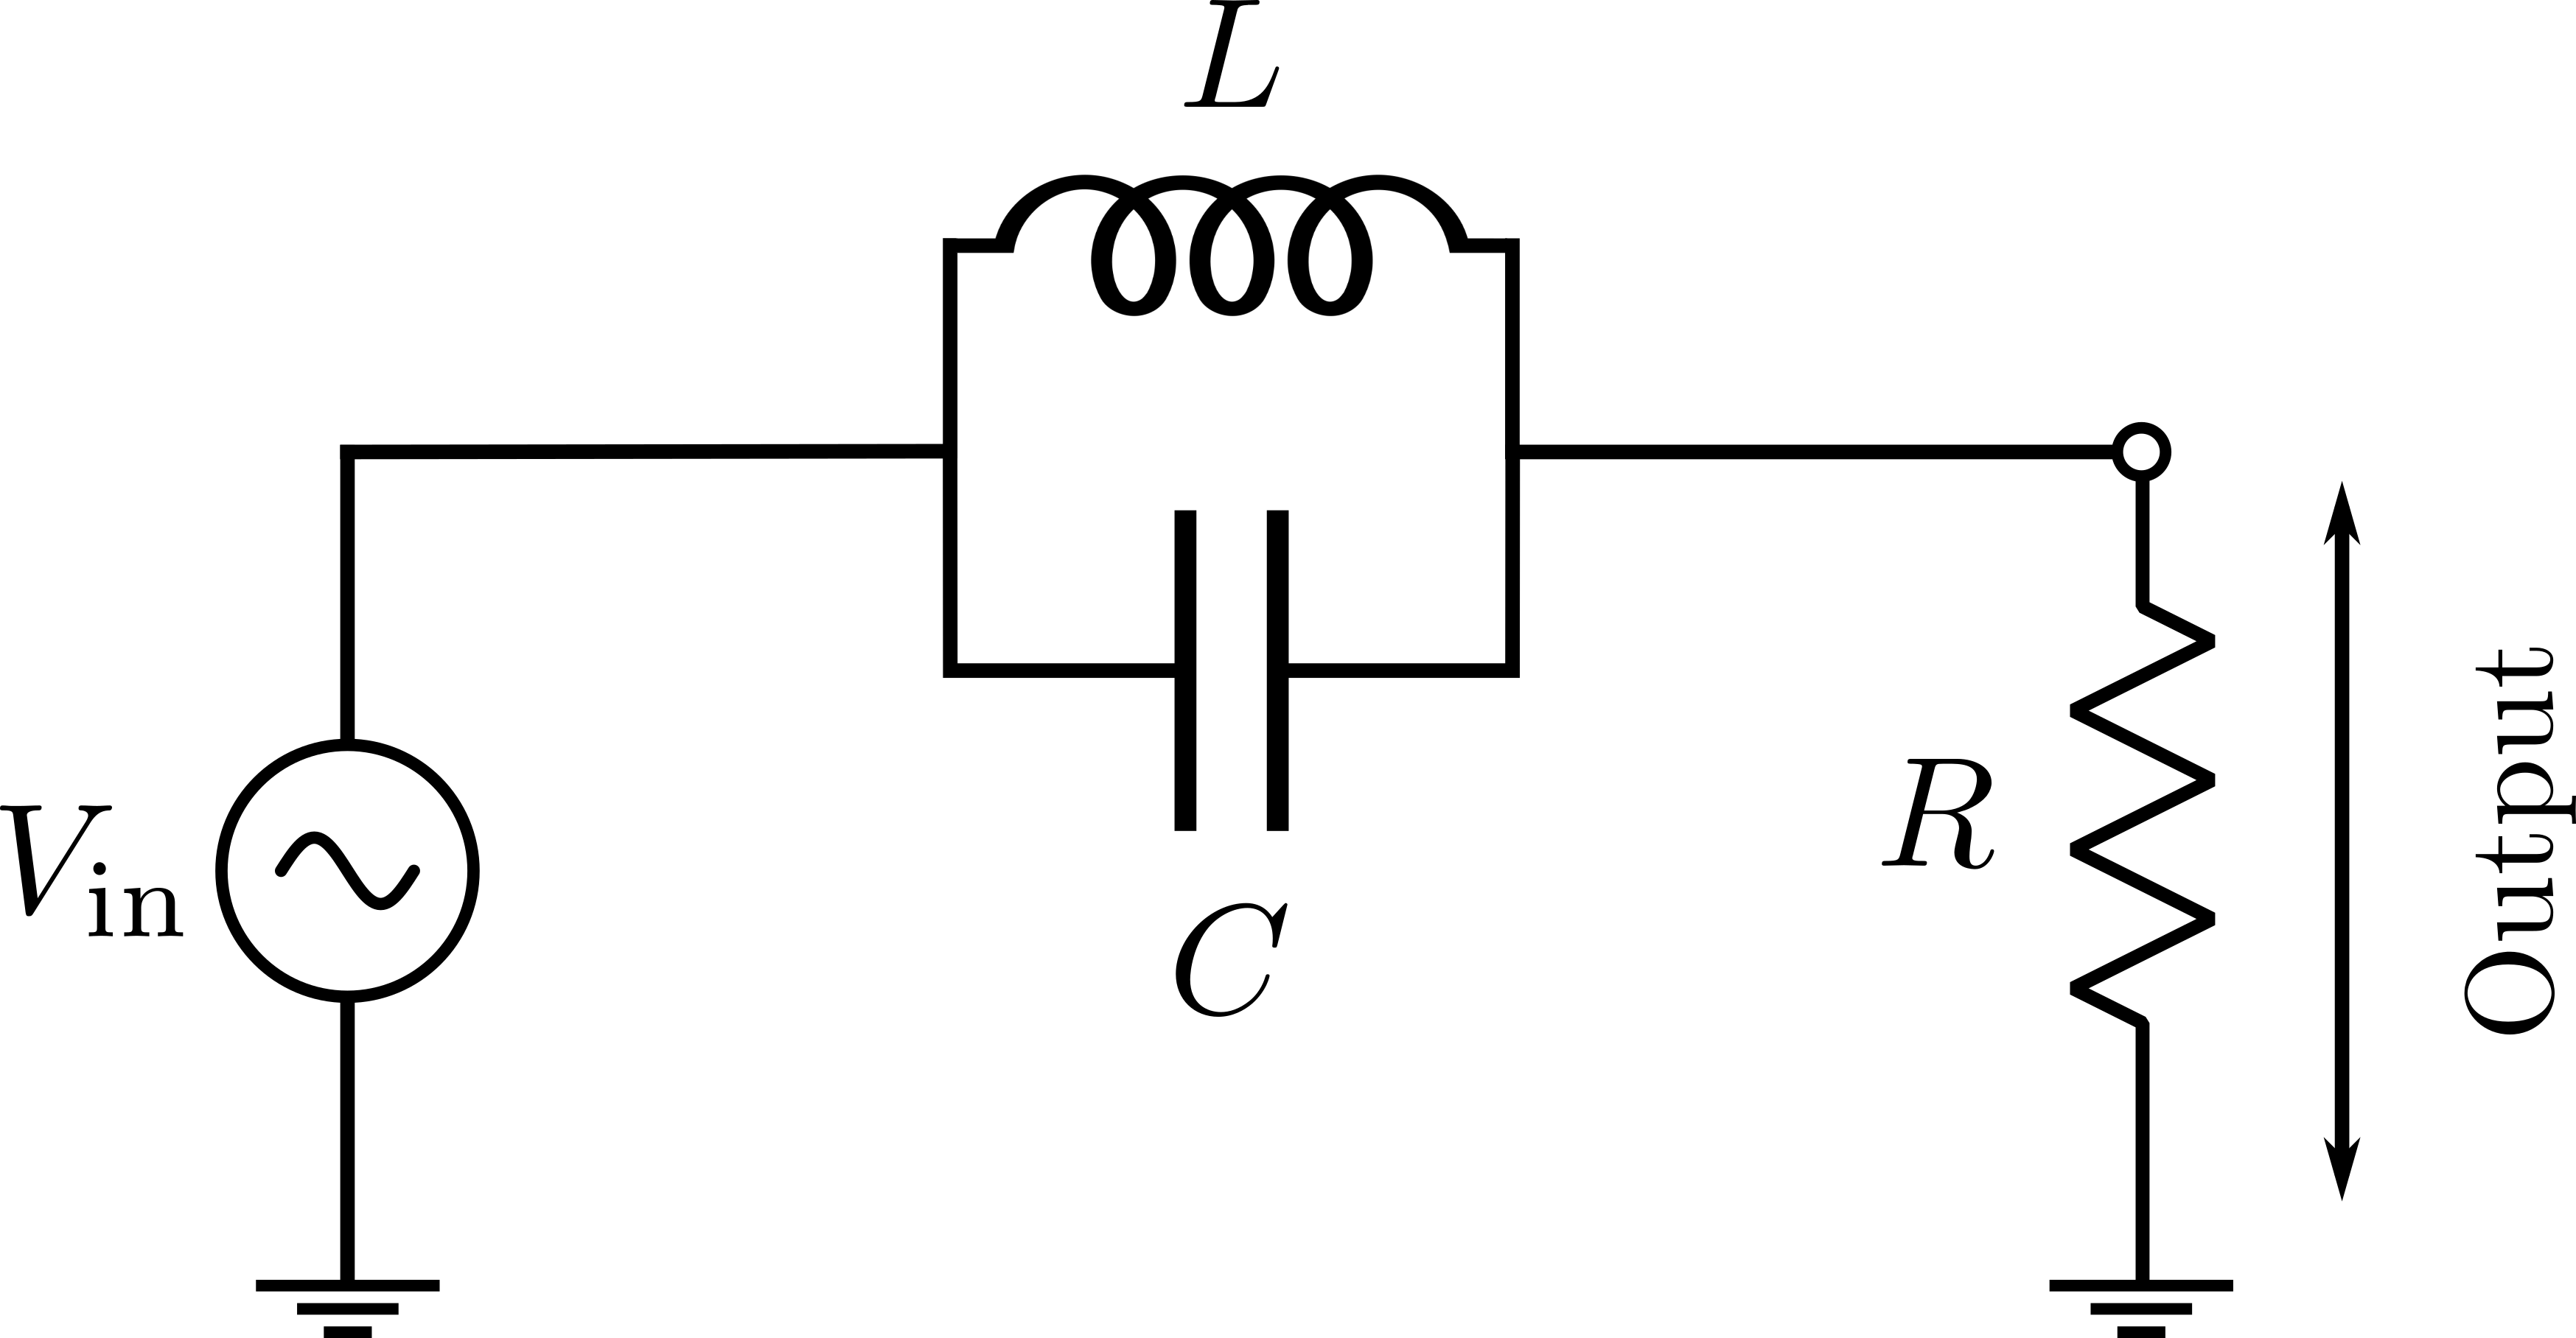
\includegraphics[width=0.65\textwidth]{figs/electronics-circuits/LCRParallel.png}
    \caption{One possible parallel configuration, known as a \textsl{tank} circuit. The inductor and the capacitor are connected in parallel, and the resistor is attached in series. An AC power supply is connected across the circuit, and the output voltage is taken across the resistor. }
    \label{fig:lcr-parallel}
\end{figure}

\begin{question}
    \textbf{Question:} As before, show that resonance occurs when $\omega = \omega_0$, just as in the series $LCR$ circuit.
    
    \textbf{Question:} Show that in the tank circuit (i) the net impedance is $0$ at both $\omega \to 0$ and $\omega\to\infty$, and (ii) at resonance, the net impedance is infinite. What does this mean for the current at resonance?
\end{question}


\subsubsection*{Phase shift around resonance}

Let us now understand exactly what happens around resonance. Consider the series $LCR$ circuit. As can be seen, resonance occurs when the complex part of the impedance goes to zero. In this case, the impedance is purely real -- the circuit is a pure resistor. Thus, when resonance occurs in such a circuit, the effect of the capacitor is exactly cancelled out by the effect of the inductor. However, as we have seen earlier, the inductor causes the current to lag behind the input voltage by a phase of $\pi/2$, while the capacitor causes the current to \textsl{lead} the voltage by the same phase of $\pi/2$. Therefore, at resonance, we would expect the current to be exactly in phase with the input voltage!

This can be detected by plotting a graph of the voltage against the current. Since for a sinusoidal signal these functions are in general out of phase at some arbitrary frequency $\omega \neq \omega_0$, we get what is known as a ``Lissajous'' figure: a superposition of two perpendicular out-of-phase sinusoidally varying functions, as shown in Figure~(\ref{fig:lissajous}). Since our frequencies are all the same, our Lissajous figures are all ellipses. The Lissajous figure can be used to determine the \textsl{phase} difference between the two signals by measuring the quantities $a$ and $b$ shown in Figure~(\ref{fig:lissajous}), where $a$ is the (positive) value of $x$ when $y=0$, and $b$ is the maximum value of $x$. 

The Lissajous figure can also be used to detect resonance, since at resonance the phase-difference is zero, meaning that the ellipse simply becomes a straight line. In other words, at resonance $a\to 0$.

\begin{figure}[!htb]
    \centering
    
\includegraphics[width=0.4\textwidth]{figs/electronics-circuits/lissajous.png}
    \caption{A Lissajous figure. The input voltage is sent across one of the channels of an oscilloscope, and the voltage across the resistor is sent across the other channel. In the \texttt{XY} mode of the oscilloscope, an ellipse is obtained. $a$ is the positive value of $x$ where $y=0$, and $b$ is the maximum value of $x$ that the ellipse can have. Using $a$ and $b$, the phase difference between the signals can be measured. }
    \label{fig:lissajous}
\end{figure}

\begin{question}
    \textbf{Question:} Consider two orthogonal sinusoids with a frequency $\omega$ and phase difference $\varphi$:
    \begin{equation}
        \begin{aligned}
            x(t) &= A \sin(\omega t + \varphi)\\
            y(t) &= B \sin(\omega t).
        \end{aligned}
    \end{equation}
    Using the above definitions, show that if
    \begin{equation}
        \begin{aligned}
            y(t)&=0 \quad \quad \implies \quad \quad a = A \sin\varphi, \\
            x(t)&=0 \quad \quad \implies \quad \quad b = A.
        \end{aligned}
    \end{equation}

    Use this to show that 
    \begin{equation}
        \varphi = \arcsin\left(\frac{a}{b}\right).
    \end{equation}
\end{question}

\begin{imp}
    \textbf{Important:} In our analysis of the $LCR$ circuit so far, you should notice that unlike the $RC$ circuit, the quantity of interest is the \textsl{current} in the circuit rather than the voltage. Our Digital Oscilloscopes, like most oscilloscopes, measures voltage, and not current. In order to get around this, we measure instead the voltage across the resistor $R$, since $V_R = I R$, and the current in the circuit is simply $I = V_R/R$. Thus, in both the series $LCR$ and ``tank'' circuits described above, the resistor also plays the role of a \textsl{load}.
\end{imp}



\section*{Experimental Setup}

\subsection*{Apparatus}

\begin{enumerate}[label=\arabic*)]
\itemsep0em
\item An assorted set of resistors, capacitors, and inductors
\item A breadboard in which to attach them
\item A function generator
\item A Digital Storage Oscilloscope (DSO)
\item BNC cables
\item A BNC T-connector

\vspace{\parskip}
\begin{imp}
\textbf{Note:}
\begin{itemize}
    \item The output on the screen of the oscilloscope can be saved to a pen-drive. This will be particularly useful if you want to save the input and output waveforms in the case of the integrator and differentiator circuits, for example.
    \item The BNC T-connector can be used to split the signal generated by the function generator into two arms. One arm can be used as the input to the circuit, while the other can be displayed on the oscilloscope. This way, both the input signal and the output signals can be observed on different channels simultaneously.
    \item In all of our analysis so far, we have used \textsl{angular} frequency $\omega$. However, the frequencies produced by the function generator and detected by the DSO are \textsl{linear} frequencies $f$. The relationship between the two is simply
    \begin{equation}
        \omega = 2 \pi f.
    \end{equation}
\end{itemize}
\end{imp}

\end{enumerate}

\subsection*{Precautions}

\begin{itemize}
\item Check the value of each of the component that you will be using \textsl{before} making the circuit, and calculate all the relevant frequencies ($\omega_c$, $\omega_0$) theoretically to make sure they lie in a reasonable range.
\item At both the cutoff and resonant frequencies, the frequency response of our circuits varies very slowly. Consequently, you should vary the frequency in smaller intervals near these regions, so that the behaviour can be seen clearly.
\item Keep the amplitude of the input signal fixed while changing the frequency.
\item Handle the DSO carefully as it is an expensive piece of equipment.
\end{itemize}


\section*{Procedure}

\subsection*{Part A}

In this part of the experiment, you will be studying the $RC$ circuit in the time-domain, and seeing how it can be used as an integrator and a differentiator. 

\begin{enumerate}
    \item Connect the resistor and the capacitor in series as shown in Figure~(\ref{fig:rc-lp}) measure the voltage across the resistor $V_R$.
    \item Connect the function generator to the input of the circuit and the DSO across the output.
    \begin{imp}
        \textbf{Note:} In every case, the voltage has to be taken \textsl{with respect to the ground}, as shown in Figure~(\ref{fig:rc-lp}). This could require some moving about of the components in your circuit.
    \end{imp}

    You can split the input using the BNC T-connector and display both $V_\text{in}$ and $V_\text{out}$ on the oscilloscope.
    \item Feed in a square-wave into the circuit, and observe the output voltage. Show that in the appropriate regime, the output voltage is the integral of the input voltage.

    \item Now repeat the same process for the circuit shown in Figure~(\ref{fig:rc-hp}), and show that in this case, the output voltage is the \textsl{derivative} of the input voltage.

    \item Store these output waveforms and include them in your final report.
\end{enumerate}


\subsection*{Part B}

Using the same two configurations as in \textbf{Part A}, you will now study the $RC$ circuit in the frequency-domain, and observe its frequency response.

\begin{enumerate}
    \item Feed a sinusoidal signal into the $RC$ circuit in the low-pass configuration. Choose a frequency such that $\omega \ll \omega_c$, the cutoff frequency for the system.
    \item Measure the ratio of the output voltage to the input voltage, and use it to compute the gain in dB.
    \item Slowly vary the frequency from $\omega \ll \omega_c$ to $\omega \gg \omega_c$, computing the gain at every value.
    \item Plot a Bode plot for the low-pass filter, and compare it to Figure~(\ref{fig:RC-bode}).
    \item Repeat the above process for the high-pass filter configuration.
\end{enumerate}

\subsection*{Part C}

We will now study the frequency response of the $LCR$ circuit in both the series and the parallel ``tank'' configuration.

\begin{enumerate}
    \item Connect the inductor, resistor, and capacitor as shown in Figure~(\ref{fig:lcr-series}), and measure the voltage across the resistor $V_R$. Remember that this is a measure of the \textsl{current} in the circuit.
    \item Feed a sinusoidal signal of frequency $\omega \ll \omega_0$, the natural frequency of the oscillator. Keep the amplitude of the input waveform fixed and vary its frequency, measuring the gain at every step.
    \item Plot a Bode plot for the frequency response of the series $LCR$ circuit.
    
    \item Similarly, make the connections for tank circuit, as shown in Figure~(\ref{fig:lcr-parallel}), and plot a similar Bode plot for its frequency response.
    \item Show that the frequency response of both the $LCR$ circuits described above appear inverted with respect to each other.
\end{enumerate}

%%%%%%%%%%%%%%%%%%%%%%
% TO INCLUDE LATER
%%%%%%%%%%%%%%%%%%%%%%

% \vbox{
% \textcolor{Blue}{\part{Appendices}}
% \tikz[remember picture,overlay]\node[shift={(-1,1)},opacity=0.6] at (current page.south east) {
\includegraphics[width=17.5cm]{logo}};
% }

% \renewcommand{\chaptername}{Appendix}

% \input{Appendix_1.tex}
% \input{Appendix_2.tex}

\end{document}